
%========= File containing the main LaTex document ========%
%                                                          %
% Copyright (C) ISI - All Rights Reserved                  %
% Proprietary                                              %
% Written by Med Hossam <med.hossam@gmail.com>, April 2016 %
%                                                          %
% @author: HEDHILI Med Houssemeddine                       %
% @linkedin: http://tn.linkedin.com/in/medhossam           %
%==========================================================%

%\documentclass[pfe]{./tpl/isipfe}
\documentclass[]{isipfe}
\graphicspath{{./img/}}

%\usepackage{hyperref}


%=========== File containing some new commands ============%
%                                                          %
% Copyright (C) ISI - All Rights Reserved                  %
% Proprietary                                              %
% Written by Med Hossam <med.hossam@gmail.com>, April 2016 %
%                                                          %
% @author: HEDHILI Med Houssemeddine                       %
% @linkedin: http://tn.linkedin.com/in/medhossam           %
%==========================================================%

\newenvironment{changemargin}[2]{%
\begin{list}{}{%
\setlength{\leftmargin}{#1}%
\setlength{\rightmargin}{#2}%
}%
\item[]}
{\end{list}}

\makeatletter

%================= front cover variables =================%

\newcommand{\secondAuthor}[1]{\gdef\@secondAuthor{#1}}%
\newcommand{\@secondAuthor}{\@latex@warning@no@line{No \noexpand\secondAuthor given}}

\newcommand{\diplomaName}[1]{\gdef\@diplomaName{#1}}%
\newcommand{\@diplomaName}{\@latex@warning@no@line{No \noexpand\diplomaName given}}

\newcommand{\speciality}[1]{\gdef\@speciality{#1}}%
\newcommand{\@speciality}{\@latex@warning@no@line{No \noexpand\speciality given}}

\newcommand{\proFramerNameOne}[1]{\gdef\@proFramerNameOne{#1}}%
\newcommand{\@proFramerNameOne}{\@latex@warning@no@line{No \noexpand\proFramerNameOne given}}

\newcommand{\proFramerSpecialityOne}[1]{\gdef\@proFramerSpecialityOne{#1}}%
\newcommand{\@proFramerSpecialityOne}{\@latex@warning@no@line{No \noexpand\proFramerSpecialityOne given}}

\newcommand{\proFramerNameTwo}[1]{\gdef\@proFramerNameTwo{#1}}%
\newcommand{\@proFramerNameTwo}{\@latex@warning@no@line{No \noexpand\proFramerNameTwo given}}

\newcommand{\proFramerSpecialityTwo}[1]{\gdef\@proFramerSpecialityTwo{#1}}%
\newcommand{\@proFramerSpecialityTwo}{\@latex@warning@no@line{No \noexpand\proFramerSpecialityTwo given}}

\newcommand{\academicFramerName}[1]{\gdef\@academicFramerName{#1}}%
\newcommand{\@academicFramerName}{\@latex@warning@no@line{No \noexpand\academicFramerName given}}

\newcommand{\academicFramerSpeciality}[1]{\gdef\@academicFramerSpeciality{#1}}%
\newcommand{\@academicFramerSpeciality}{\@latex@warning@no@line{No \noexpand\academicFramerSpeciality given}}

\newcommand{\collegeYear}[1]{\gdef\@collegeYear{#1}}%
\newcommand{\@collegeYear}{\@latex@warning@no@line{No \noexpand\collegeYear given}}

\newcommand{\companyName}[1]{\gdef\@companyName{#1}}%
\newcommand{\@companyName}{\@latex@warning@no@line{No \noexpand\companyName given}}

%================== Signatures variables ==================%

\newcommand{\proSignSentence}[1]{\gdef\@proSignSentence{#1}}%
\newcommand{\@proSignSentence}{\@latex@warning@no@line{No \noexpand\proSignSentence given}}

\newcommand{\academicSignSentence}[1]{\gdef\@academicSignSentence{#1}}%
\newcommand{\@academicSignSentence}{\@latex@warning@no@line{No \noexpand\academicSignSentence given}}

%================== Backcover variables ==================%

\newcommand{\arabicAbstract}[1]{\gdef\@arabicAbstract{#1}}%
\newcommand{\@arabicAbstract}{\@latex@warning@no@line{No \noexpand\arabicAbstract given}}

\newcommand{\arabicAbstractKeywords}[1]{\gdef\@arabicAbstractKeywords{#1}}%
\newcommand{\@arabicAbstractKeywords}{\@latex@warning@no@line{No \noexpand\arabicAbstractKeywords given}}

\newcommand{\frenchAbstract}[1]{\gdef\@frenchAbstract{#1}}%
\newcommand{\@frenchAbstract}{\@latex@warning@no@line{No \noexpand\frenchAbstract given}}

\newcommand{\frenchAbstractKeywords}[1]{\gdef\@frenchAbstractKeywords{#1}}%
\newcommand{\@frenchAbstractKeywords}{\@latex@warning@no@line{No \noexpand\frenchAbstractKeywords given}}

\newcommand{\englishAbstract}[1]{\gdef\@englishAbstract{#1}}%
\newcommand{\@englishAbstract}{\@latex@warning@no@line{No \noexpand\englishAbstract given}}

\newcommand{\englishAbstractKeywords}[1]{\gdef\@englishAbstractKeywords{#1}}%
\newcommand{\@englishAbstractKeywords}{\@latex@warning@no@line{No \noexpand\englishAbstractKeywords given}}

\newcommand{\companyEmail}[1]{\gdef\@companyEmail{#1}}%
\newcommand{\@companyEmail}{\@latex@warning@no@line{No \noexpand\companyEmail given}}

\newcommand{\companyTel}[1]{\gdef\@companyTel{#1}}%
\newcommand{\@companyTel}{\@latex@warning@no@line{No \noexpand\companyTel given}}

\newcommand{\companyFax}[1]{\gdef\@companyFax{#1}}%
\newcommand{\@companyFax}{\@latex@warning@no@line{No \noexpand\companyFax given}}

\newcommand{\companyAddressFR}[1]{\gdef\@companyAddressFR{#1}}%
\newcommand{\@companyAddressFR}{\@latex@warning@no@line{No \noexpand\companyAddressFR given}}

\newcommand{\companyAddressAR}[1]{\gdef\@companyAddressAR{#1}}%
\newcommand{\@companyAddressAR}{\@latex@warning@no@line{No \noexpand\companyAddressAR given}}

%============= cmd for inserting blank page =============%
\newcommand\blankpage{%
    \null
    \thispagestyle{empty}%
    \addtocounter{page}{-1}%
    \newpage}

%================ document main language ================%
\selectlanguage{english}
%\selectlanguage{french}

%================== required packages ===================%

\usepackage{enumerate}  

\usepackage{tcolorbox}
\usepackage{afterpage}
\usepackage{array,longtable,multirow}% http://ctan.org/pkg/{array,longtable,multirow}
\usepackage{pifont}

\usepackage{pdflscape}
\usepackage{rotating}
\usepackage{wrapfig}

% @author: Stoufa
% the command `\makeindex` is mandatory to create the index file main.idx
% https://tex.stackexchange.com/questions/9913/input-index-file-not-found
\makeindex
\begin{document}
    
%=== File containing Global Configuration of the report ===%
%                                                          %
% Copyright (C) ISI - All Rights Reserved                  %
% Proprietary                                              %
% Written by Med Hossam <med.hossam@gmail.com>, April 2016 %
%                                                          %
% @author: HEDHILI Med Houssemeddine                       %
% @linkedin: http://tn.linkedin.com/in/medhossam           %
%==========================================================%

%=========== You MUST type your information here ==========%
% global_config.tex file is designed to configure your     %
% cover pages (main, back and black covers)                %
%==========================================================%

%============= Config new columns type ==============%
\newcolumntype{L}{>{\raggedright\arraybackslash}}
\newcolumntype{R}{>{\raggedleft\arraybackslash}}
\newcolumntype{C}{>{\centering\arraybackslash}}
%==================================================%

%========= Config the cover section ==========%

\title{Running Coremark on STM32 devices using Csolution project structure }

\author{Youssef HASNAOUI}
%%% if necessary
% Set isBinomal to true and type second author name
%\setboolean{isBinomal}{true}
%\secondAuthor{Prénom NOM}

\diplomaName{National Diploma in Infotronics Systems Engineering}
\speciality{Embedded Systems}
%\speciality{Génie des Télécommunications et Réseaux}
%\speciality{Génie Informatique des Systèmes Industriels}

%% Encadrant professionnel
\proFramerNameOne{Mohamed HAMROUNI}
\proFramerSpecialityOne{Application Engineer}


%% Entreprise d'accueil
\companyName{STMicroelectronics}

%% Année universitaire
\collegeYear{2024 - 2025}

%%%%%% Signatures section %%%%%%

% You can simply remove theses sentences by typing an empty string
% \proSignSentence{}

\proSignSentence{J'autorise l'étudiant à faire le dépôt de son rapport de stage en vue d'une soutenance.}


%%% AR

%% To use latin characters inside the arabic text
% just put them inside the command \textLR{}
%%%%

%%% FR
\frenchAbstract{Ce rapport décrit les travaux réalisés lors de mon stage d'été chez STMicroelectronics, axé sur l'analyse comparative indépendante de la plateforme. L'objectif principal était d'exécuter Coremark sur des microcontrôleurs STM32 en utilisant la structure de projet Csolution. Pour ce faire, j'ai mis à profit mes connaissances en développement logiciel et embarqué, en compilation et génération de code C, à l'aide d'outils tels que CMSIS-Toolbox, C et Golang. Les résultats ont permis de réduire considérablement le temps nécessaire à la configuration et à l'exécution des projets Coremark avec plusieurs compilateurs, tout en optimisant les résultats. Ce stage m'a également permis de renforcer mes compétences en compilation, en conception d'architecture de projets embarqués et de mieux comprendre les défis spécifiques de l'ingénierie des systèmes embarqués.}

\frenchAbstractKeywords{C/C++, Golang, Systèmes embarqués, STM32, Compilation, Génération de Code.}

%% dont go over 10 lines
%%% EN
\englishAbstract{This report describes the work carried out during my summer internship at STMicroelectronics, focused on platform-agnostic benchmarking. The main objective was to run Coremark on STM32 devices using Csolution project structure. To achieve this, I put to use my knowledge in software and embedded development,C code compilation and code generation, using tools such as CMSIS-Toolbox, C and Golang. The results helped to drastically reduce the time required to setup and run Coremark projects using multiple compilers, as well as generating the most optimal results. This internship also allowed me to strengthen my skills in the compilation process, embedded projects architecture design and gain insight into the specific challenges of embedded systems engineering.}

\englishAbstractKeywords{C/C++, Golang, Embedded Systems, STM32, Compilation, Code Generation.}

%% if you want to get rid of the company address just set the boolean variable to false
% PS : it's optional
\setboolean{wantToTypeCompanyAddress}{false}

\companyEmail{contact@company.com}
\companyTel{71 111 111}
\companyFax{71 222 222}
\companyAddressAR{نهج بحيرة ملاران - ضفاف البحيرة - تونس}
\companyAddressFR{Rue du Lac Malaren, Les Berges du Lac 1053 Tunis}
    
    \frontmatter
        \thispagestyle{cover}%
\newgeometry{bottom=25mm,left=20mm,top=15mm,right=20mm}
\hspace{-47pt}
\begin{minipage}[l]{0.2\columnwidth}
    \vspace{6mm}
    
\includegraphics[width=1.1\columnwidth]{img/ensit logo.png}\\
\end{minipage}
\hfill
\begin{minipage}[l]{0.6\columnwidth}
    \centering
    \footnotesize
    \textbf{{Republic of Tunisia}}\\
    \vspace{1.5mm}
    \textbf{{Ministry of Higher Education\\
                and Scientific Research}}\\
    \vspace{1.5mm}
    \textbf{{University of Carthage }}\\
    \vspace{1.5mm}
    \textbf{{National Engineering School of Carthage}}
\end{minipage}
\hfill
\begin{minipage}[l]{0.02\columnwidth}
\end{minipage}
\hfill
\begin{minipage}[l]{0.18\columnwidth}
    \vspace{6mm}
    
\includegraphics[width=1.1\columnwidth]{img/UT PNG.png}\\
\end{minipage}
\vskip1.5cm

\begin{center}
    {\LARGE{\textbf{\textsc{Summer Internship Project Report}}}}\\
    \vskip0.5cm
    \large

\end{center}

\begin{center}
    \textrm{By}\\
    \vskip0.3cm
    {\ifthenelse{\boolean{isBinomal}}
    {% IF TRUE
        \begin{center}
            \large\textbf{\@author}~~~~~ et ~~~~~
            \large\textbf{\@secondAuthor}
        \end{center}
    }
    {\Large\textbf{\@author}}% FALSE
    }
    \vskip12mm

    \definecolor{isiBlue}{RGB}{31, 78, 121}

    \begin{changemargin}{-9mm}{0cm}
        \begin{minipage}[l]{1.1\columnwidth}
            \begin{tcolorbox}[colframe=black,colback=white,boxrule=0pt,toprule=3pt,bottomrule=3pt,arc=0pt,top=0mm,right=0mm,left=0mm,bottom=0mm,boxsep=0.5mm]{
                    \begin{tcolorbox}[colframe=black,colback=white, boxrule=0pt,toprule=1pt,bottomrule=1pt,arc=0pt,enlarge bottom by=-0.9mm, auto outer arc]
                        \centering
                        {\huge\textbf{\@title }}
                    \end{tcolorbox}
                }
            \end{tcolorbox}
        \end{minipage}
    \end{changemargin}

\end{center}
\vskip8mm%

\begin{center}
    \large
    \begin{minipage}[c]{0.28\columnwidth}
        Professional supervisor:
        \newline
    \end{minipage}
    \hfill
    \begin{minipage}[c]{0.42\columnwidth}
        \textbf{\@proFramerNameOne}\\
    \end{minipage}
    \hfill

\end{center}
\vskip16mm

\begin{center}
    \large
    Project Elaborated Within \@companyName\\
    \vskip0.2cm

    \begin{figure}[h]
        \centering
        {\color{black}{\fboxrule=2.5pt\fbox{
\includegraphics[width=0.43\columnwidth]{img/ST_logo_2024_blue.jpg}}}}
    \end{figure}
\end{center}
\afterpage{\blankpage}

        %
%===== File containing the black cover of the document ====%
%                                                          %
% Copyright (C) ISI - All Rights Reserved                  %
% Proprietary                                              %
% Written by Med Hossam <med.hossam@gmail.com>, April 2016 %
%                                                          %
% @author: HEDHILI Med Houssemeddine                       %
% @linkedin: http://tn.linkedin.com/in/medhossam           %
%==========================================================%

%== It's advised to not modify the content of this file ===%
% To set your information, go to global_config.tex file    %
%==========================================================%

\thispagestyle{cover}%
\hspace{-47pt}
\begin{minipage}[l]{0.2\columnwidth}
\vspace{6mm}

\includegraphics[width=1.1\columnwidth]{Logo_ISI_Black}\\
\end{minipage}
\hfill
\begin{minipage}[l]{0.6\columnwidth}
\centering
\footnotesize
\textbf{{République Tunisienne}}\\
\vspace{1.5mm}
\textbf{{Ministère de l'Enseignement Supérieur\\
et de la Recherche Scientifique}}\\
\vspace{1.5mm}
\textbf{{Université de Tunis El Manar}}\\
\vspace{1.5mm}
\textbf{{Institut Supérieur d'Informatique d’El Manar}}
\end{minipage}
\hfill
\begin{minipage}[l]{0.02\columnwidth}
\end{minipage}
\hfill
\begin{minipage}[l]{0.18\columnwidth}
\vspace{6mm}

\includegraphics[width=0.9\columnwidth]{Logo_UTM_Black}\\
\end{minipage}
\vskip1.5cm

\begin{center}
{\LARGE{\textbf{\textsc{Rapport de Projet de Fin d'\'Etudes}}}}\\
\vskip0.5cm
\large

{\textbf{Présenté en vue de l'obtention du}}\\
\vskip2mm
{\textbf{\@diplomaName}}\\
{\textbf{Spécialité : \@speciality}}\\
{}
\end{center}

\begin{center}
\textrm{Par}\\
\vskip0.3cm
{\ifthenelse{\boolean{isBinomal}}
    {% IF TRUE
        \begin{center}
            \large\textbf{\@author}~~~~~ et ~~~~~
            \large\textbf{\@secondAuthor}
        \end{center}
    }
    {\Large\textbf{\@author}}% FALSE
}
\vskip12mm

\begin{changemargin}{-9mm}{0cm}
\begin{minipage}[l]{1.1\columnwidth}
\begin{tcolorbox}[colback=white,boxrule=0pt,toprule=3pt,bottomrule=3pt,arc=0pt,top=0mm,right=0mm,left=0mm,bottom=0mm,boxsep=0.5mm]{
    \begin{tcolorbox}[colback=white, boxrule=0pt,toprule=1pt,bottomrule=1pt,arc=0pt,enlarge bottom by=-0.9mm, auto outer arc]
        \centering
        {\huge\textbf{\@title}}
    \end{tcolorbox}
}
\end{tcolorbox}
\end{minipage}
\end{changemargin}

\end{center}
\vskip8mm%

\begin{center}
\large
\begin{minipage}[c]{0.28\columnwidth}
Encadrant professionnel:\\
Encadrant académique:
\end{minipage}
\hfill
\begin{minipage}[c]{0.42\columnwidth}
\textbf{\@proFramerName}\\
\textbf{\@academicFramerName}
\end{minipage}
\hfill
\begin{minipage}[c]{0.26\columnwidth}
\@proFramerSpeciality\\
\@academicFramerSpeciality
\end{minipage}
\end{center}
\vskip16mm

\begin{center}
\large
Réalisé au sein de \@companyName\\
\vskip0.4cm
\begin{figure}[h]
\centering
{{\fboxrule=2.5pt\fbox{
\includegraphics[width=0.4\columnwidth]{Logo_Entreprise_Black}}}}
\end{figure}
\end{center}

\restoregeometry
        %\thispagestyle{empty}

% \begin{center}
%     \begin{minipage}[l]{1\columnwidth}
%         \begin{tcolorbox}[colback=white,boxrule=5pt,arc=10pt,height=105mm]{
%             \vspace{2cm}
%             \large \@proSignSentence
%             \vspace{1mm}
%             \begin{center}
%                 \Large
%                 Encadrant professionnel, \textbf{\@proFramerName}
%             \end{center}
%             \vspace{5mm}
%             \hspace{0.71\columnwidth}\textbf{\large Signature et cachet}
%         }
%         \end{tcolorbox}
%     \end{minipage}
    
%     \vspace{2cm}
    
%     \begin{minipage}[l]{1\columnwidth}
%         \begin{tcolorbox}[colback=white,boxrule=5pt,arc=10pt,height=105mm]{
%             \vspace{2cm}
%             \large \@academicSignSentence
%             \vspace{1mm}
%             \begin{center}
%                 \Large
%                 Encadrant académique, \textbf{\@academicFramerName}
%             \end{center}
%             \vspace{5mm}
%             \hspace{0.84\columnwidth}\textbf{\large Signature}
%         }
%         \end{tcolorbox}
%     \end{minipage}
% \end{center}

        
        \setcounter{page}{0}
        \chapter*{\Huge Dedications}

\begingroup
\begin{center}
    \it \LARGE
I dedicate this work to my family and friends.

 
To my mother \textbf{Monia Sellami}, your love and support means so much to me in every step of my journey. You're the best.

To my father \textbf{Makram Hasnaoui}, thank you so much for all the sacrifices you've made for my sake. I could never be here without you.


To my sister \textbf{Aicha}, your kindness and your belief in me have been a constant source of inspiration, and for that, I am very grateful.

To my friends, you have my most sincere %reaction
gratitude for your support, your guidance and your company throughout this journey. 

    \vspace{4mm}
\end{center}

\endgroup

\vspace{8mm}
\begin{flushright}
    \Large Thank you,\\
    \LARGE \@author
\end{flushright}
        \thispagestyle{frontmatter}
        \chapter*{\huge Acknowledgements}

\begin{center}
    \it \LARGE
    I would like to sincerely thank everyone who had a hand in the development of this project.

    Firstly, I want to express my utmost appreciation to \textbf{Mohamed HAMROUNI}, his guidance and support has been invaluable, and has kept me motivated and determined to give my best effort.

    Last but not least, to every single person that contributed to the successful completion of this project with their constant support and motivation, you have my utmost thanks.
\end{center}
        \thispagestyle{frontmatter}
        
        \setcounter{secnumdepth}{3}
        \setcounter{tocdepth}{2}
        \dominitoc
        \tableofcontents
        \adjustmtc
        \thispagestyle{frontmatter}
        %uncomment from here ----
       \listoffigures
        \thispagestyle{frontmatter}
        \listoftables
        \thispagestyle{frontmatter}
        %to here  ----
        \chapter*{List of Acronyms}

%=============== Glossary example ==============%
% it's an enhanced itemize list to make it      %
% sortable automatically.                       %
%===============================================%

\begin{acronyms}


    \sortitem[MCU]{
        \textbf{M}icro \textbf{C}ontroller \textbf{U}nit
    }
    
     \sortitem[IV]{
        \textbf{I}nitialization \textbf{V}ector
    }
    \sortitem[HAL]{
        \textbf{H}ardware \textbf{A}bstraction \textbf{L}ayer
    }
    \sortitem[ARM]{
        \textbf{A}dvanced \textbf{R}ISC \textbf{M}achine
    }
    \sortitem[USART]{
        \textbf{U}niversal \textbf{S}ynchronous \textbf{A}synchronous 
    \textbf{R}eceiver \textbf{T}ransmitter
    }
    \sortitem[UART]{
        \textbf{U}niversal \textbf{A}synchronous 
    \textbf{R}eceiver \textbf{T}ransmitter
    }
    \sortitem[FPU]{
        \textbf{F}loating \textbf{P}oint \textbf{U}nit
    }
    \sortitem[IP]{
        \textbf{I}ntegrated \textbf{P}eripheral
    }
    \sortitem[IDE]{
        \textbf{I}ntegrated \textbf{D}evelopement \textbf{E}nvironment
    }
    \sortitem[CMSIS]{
        \textbf{C}ortex \textbf{M}icrocontroller \textbf{S}oftware \textbf{I}nterface \textbf{S}tandard
    }
    \sortitem[LL]{
        \textbf{L}ow-\textbf{L}ayer
    }
    \sortitem[GNU]{
        \textbf{G}NU's \textbf{N}ot \textbf{U}nix
    }
    \sortitem[GCC]{
        \textbf{G}NU \textbf{C}ompiler \textbf{C}ollection
    }
    \sortitem[IAR]{
        \textbf{I}ngenjörsfirma \textbf{A}nders \textbf{R}undgren
    }
    \sortitem[LLVM]{
        \textbf{L}ow \textbf{L}evel \textbf{V}irtual \textbf{M}achine
    }
    \sortitem[API]{
        \textbf{A}pplication \textbf{P}rogramming \textbf{I}nterface
    }
    \sortitem[RTOS]{
        \textbf{R}eal-\textbf{T}ime \textbf{O}perating \textbf{S}ystem
    }
    \sortitem[RTE]{
        \textbf{R}un\textbf{T}ime \textbf{E}nvironment
    }
    \sortitem[PLM]{
        \textbf{P}roject \textbf{L}ifetime \textbf{M}anagement
    }
    \sortitem[YAML]{
        \textbf{Y}et \textbf{A}nother \textbf{M}arkup \textbf{L}anguage
    }
    \sortitem[JSON]{
        \textbf{J}ava\textbf{S}cript \textbf{O}bject \textbf{N}otation
    }
    \sortitem[ELF]{
        \textbf{E}xecutable and \textbf{L}inkable \textbf{F}ormat
    }
    \sortitem[DWARF]{
        \textbf{D}ebugging \textbf{W}ith \textbf{A}ttributed \textbf{R}ecord \textbf{F}ormats
    }
    \sortitem[DFP]{
        \textbf{D}evice \textbf{F}amily \textbf{P}ack
    }
    \sortitem[BSP]{
        \textbf{B}oard \textbf{S}upport \textbf{P}pack
    }
    \sortitem[SVD]{
        \textbf{S}ystem \textbf{V}iew \textbf{D}escription
    }
    \sortitem[SCVD]{
        \textbf{S}oftware \textbf{C}omponent \textbf{V}iewer \textbf{D}escription
    }
    \sortitem[RegEx]{
        \textbf{Reg}ular \textbf{Ex}pression
    }

\end{acronyms}
        \thispagestyle{frontmatter}
    
    \mainmatter
        \chapter*{Introduction}
\addcontentsline{toc}{chapter}{Introduction} % to include the introduction to the table of content
\markboth{Introduction}{} %To redefine the section page head

In today's technological landscape, the importance of benchmarking in embedded systems cannot be overstated. Embedded systems are integral to a wide range of applications, from consumer electronics and industrial automation to healthcare devices and automotive systems. Therefore, evaluations provide objective data on performance, efficiency and reliability, making them essential for making informed design and purchasing decisions. As systems grow more complex and interconnected, the number of configurable parameters and potential performance bottlenecks expands, increasing the risk of suboptimal performance, wasted resources and failed deployments. Establishing a rigorous and standardized benchmarking methodology is therefore paramount to ensure systems meet their intended requirements and deliver value in both development and production environments.

Benchmarking provides the fundamental framework for this objective analysis by establishing a standardized set of metrics and tests to quantify a system's performance. Effective benchmarking allows developers to measure key characteristics such as processing speed, memory throughput, power consumption, and real-time task execution, creating a data-driven basis for comparison. However, executing benchmarks in embedded systems comes with challenges. Developers must navigate complexities such as isolating the unit under test, minimizing the influence of external systems, selecting appropriate tools, and ensuring that the test conditions are consistent and reproducible across different platforms and devices. Inaccurate methodology or poorly designed tests can cause misleading results, rendering the data useless for making decisions.

The dependency on proprietary and platform-specific vendor tools can lock projects into a single ecosystem and hinder reproducibility. There is a growing need to have development environments that prioritize portability and vendor independence, allowing benchmarks to be built, deployed, and executed consistently across a wide range of hardware. By abstracting away toolchain-specific complexities, such environments allow developers to focus on the benchmark results themselves rather than the intricacies of the different build processes.

This report explores the implementation of the CoreMark benchmark on STM32 devices using CMSIS-Toolbox, and the related Csolution project structure as a step towards this goal. This method demonstrates a move away from proprietary IDE-bound setups and towards a portable, platform-independent driven workflow. By leveraging a toolchain-agnostic approach, we establish a reproducible environment for evaluations. This reduces vendor lock-in, enhances cross-platform compatibility, ensures the data is a reliable reflection of the hardware capabilities, and, as a side effect, allows for a fair comparison between the available toolchains.
        \clearpage
        
        \chapter{Internship Context}
\label{chap:premierchapitre}
\section*{Internship Context}
This opening chapter focuses on introducing the host company STMicroelectronics, and provides an overview of the company's activities and global presence. It also includes an introduction to ST Tunis and the Support Solutions team, which played a pivotal role in the execution of this project, as well as an outline of the project's overall framework. Following the presentation of the challenges, we will explore the current state of the art and finally present the proposed solution which is the main objective of this project.

\section{Host Organization}
\subsection{STMicroelectronics}

STMicroelectronics (ST) is a global leader in the semiconductor industry, providing innovative solutions across various markets, including automotive, industrial, personal electronics, and communications equipment.

Founded in 1987 through the merger of SGS Microelettronica of Italy and Thomson Semiconducteurs of France, ST has grown to become one of the largest semiconductor companies in the world.

\subsection{Activity Sectors}

ST's mission is to be the undisputed leader in the semiconductor market, delivering sustainable and innovative solutions that make a positive impact on people's lives. The company's vision is to create technology that enables a more intelligent and connected world, driving progress in key areas such as smart driving, smart industry, smart home, and smart city applications.\\
The following illustration highlights the key end markets targetted by ST's solutions \cite{st_comp}.

\begin{figure}[H]
  \centering
  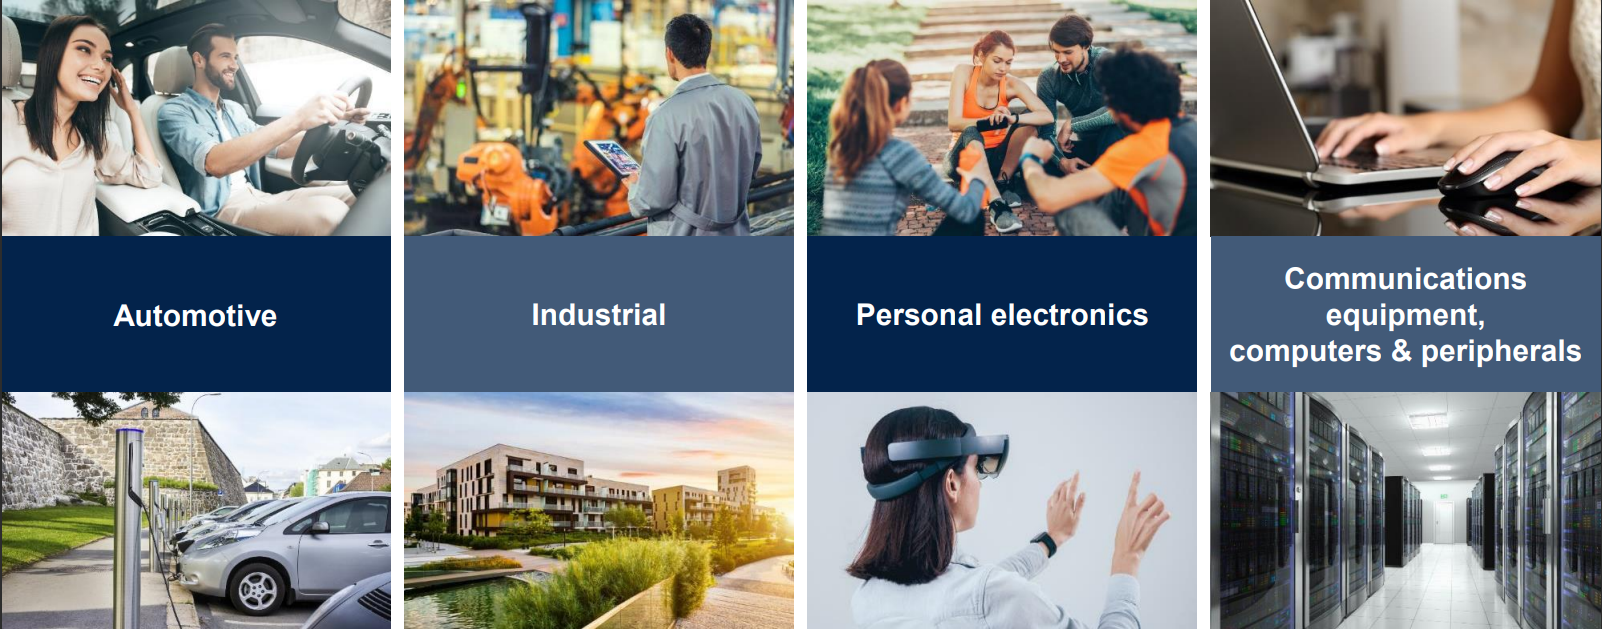
\includegraphics[width=16cm]{end markets.png}
  \caption{STMicroelectronics Activity Sectors}
  \label{fig:talan_graphe}
\end{figure}

\subsection{Global Presence}

STMicroelectronics operates in more than 35 countries, with a strong presence in key markets around the world. Figure \ref{fig:map} illustrates the company's global network, which includes \cite{st_comp}:

\begin{itemize}
    \item \textbf{Manufacturing Sites:} ST has 14 main manufacturing sites, strategically located to serve its global customer base efficiently.
    \item \textbf{Sales \& Marketing Offices:} With a network of sales and marketing offices, ST provides localized support and services to its customers.
    \item \textbf{R\&D Centers:} ST's R\&D centers are spread across the globe, fostering innovation and collaboration.
\end{itemize}

\begin{figure}[H]
  \centering
  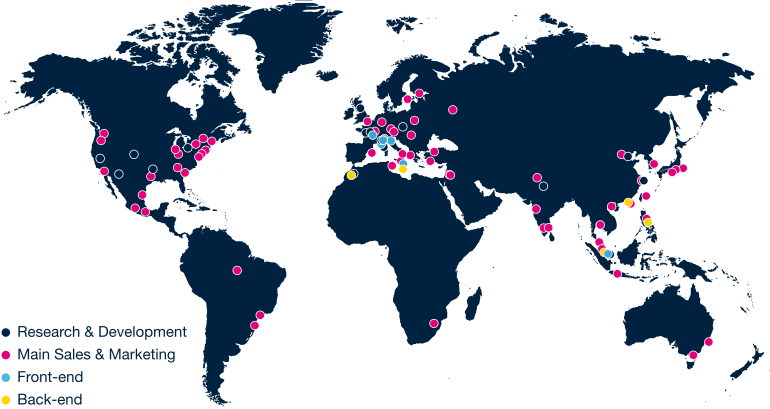
\includegraphics[width=16cm]{st map.png}
  \caption{STMicroelectronics Worldwide Presence}
  \label{fig:map}
\end{figure}

\subsection{ST Tunis}

The STMicroelectronics Tunis site, located in the El Ghazela Technopark, employs over 100 professionals in various fields such as tools, applications, quality, and support functions. The facility is involved in all stages of the microelectronics industry, from initial circuit design to final verification before mass production.

With expertise in both hardware and software, the Tunis center's activities include electronic circuit design, software tool development, application software support, and the electrical validation and verification of new circuits. This diverse skill set allows the center to contribute significantly to ST's global operations.

 \begin{figure}[htp]
  \centering
  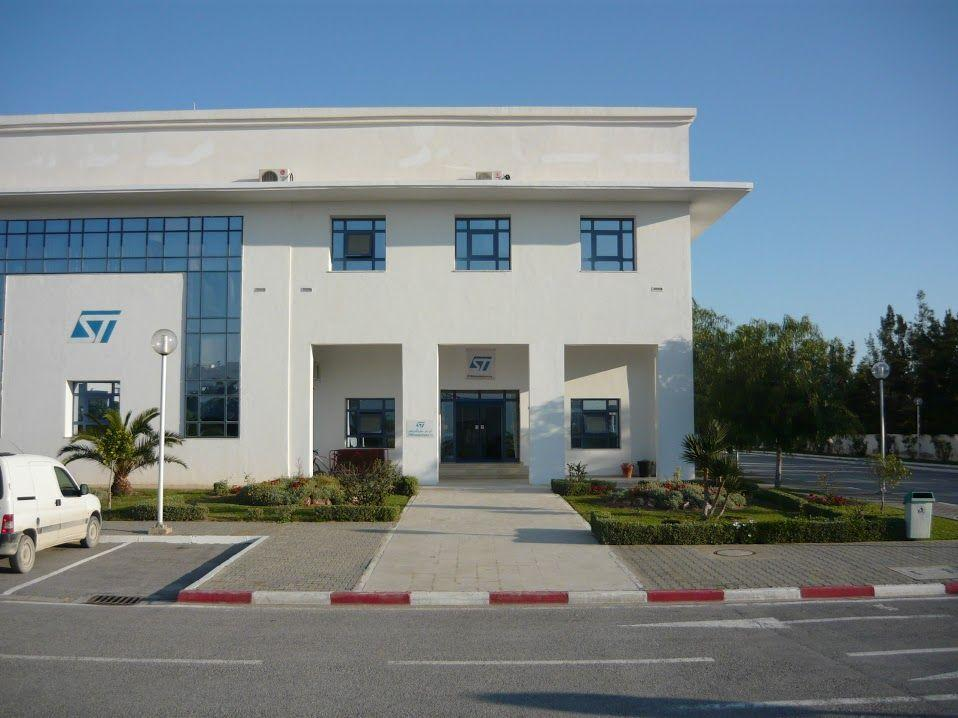
\includegraphics[width=10cm]{stmicroelectronics-tunis-site.jpg}
  \caption{STMicroelectronics Tunis}
  \label{fig:talan_graphe}
\end{figure}


\subsection{ST Support Solutions }
The ST Support Solutions team is dedicated to delivering comprehensive customer support while managing and publishing STM32 product documentation. Their role includes providing in-depth technical support for ST’s tools and products, helping customers troubleshoot problems and optimize their use of these technologies. They ensure the accuracy, clarity, and consistency of all technical documentation, which is regularly updated to reflect the latest developments and innovations. The team is also involved in enhancing and maintaining existing products, as well as defining new products, derivatives, and application references to meet evolving market needs. Additionally, they lead initiatives related to intellectual property applications, offering specific support through the development of application notes, training programs, and other resources that help customers fully understand and utilize ST’s products. This multifaceted approach ensures both customer satisfaction and continuous improvement in the STM32 ecosystem.

\section {Project Context}

Benchmarking microcontrollers is a fundamental step in evaluating their computational capabilities, power efficiency, and suitability for various applications, such as IoT, robotics, or industrial control. Among the many available benchmarks, CoreMark, developed by EEMBC, has become the de facto standard for embedded systems because it provides a well-defined, portable, and reliable performance metric.
STM32 microcontrollers, are widely adopted in the embedded systems industry due to their scalability, rich peripheral set, and performance-to-cost ratio.

The \textbf{CMSIS} initiative, led by Arm, and its Open-CMSIS-Pack ecosystem aim to standardize microcontroller development workflows. Within this ecosystem, Csolution provides a modern, metadata-driven project structure that enables cross-platform builds, device abstraction, and automation. Leveraging Csolution can significantly simplify benchmarking workflows by providing a unified and reproducible project generation and build process.

\section{Problem Statement}
Running CoreMark on STM32 devices traditionally requires manual setup for each device, including:
\begin{itemize}
	\item Creating and configuring individual projects for different STM32 families.
	\item Managing peripheral initialization.
	\item Providing a clock source to Coremark.
	\item Handling different compiler options and toolchains.
	\item Customizing linker scripts manually.
	\item Maintaining multiple project files for IDEs like Keil µVision, IAR EWARM, or others.
\end{itemize}
This manual process is time-consuming, error-prone, and non-scalable, especially when benchmarking a wide range of devices.
There is currently no standardized, automated workflow that allows developers to quickly generate CoreMark-ready projects for different STM32 targets while ensuring consistency and portability.

\section{State of the Art}
The current approaches to running benchmarks on STM32 devices typically rely on:
\begin{itemize}
	\item Vendor-Specific IDEs
		IDEs provide an easy way to manage projects via a graphical interface, they typically provide tools for peripheral configuration, memory management and compiler options.
		They also offer integrated build and debug environments.
	\item Standalone CoreMark Implementations
		EEMBC provides CoreMark source code with minimal reference implementations, it is up to the developer to manually adapt it to the target device, providing startup and initialization code, memory configuration and a clock source.
	\item Custom Build Systems
		Some environments require the use of custom build systems such as CMake and Make, these tools allow the developer to manually manage dependencies, defines and other C/C++ related build configuration.
	\item CMSIS Packs
		CMSIS packs offer a standardized way of packaging drivers, middleware and device specific files, they provide metadata to describe the device's memory and peripheral layout.
\end{itemize}
\section{Critique of Current State of the Art}

While the above methods work, they exhibit several limitations:


\begin{tabularx}{\linewidth}{@{}>{\bfseries}l X X@{}}
	\toprule
	Approach & Advantages & Limitations \\
	\midrule
	Vendor-Specific IDEs & Intuitive GUI, built-in drivers, easy to use & Projects are IDE-specific, hard to automate, poor scalability \\
	\midrule
	Standalone CoreMark & Portable reference code on computers & Significant manual effort for adaptation to each MCU \\
	\midrule
	Custom Build Systems & Flexible, automation-friendly & Requires deep expertise, no standardized metadata integration \\
	\midrule
	CMSIS Packs & Standardized packaging and metadata support & Lack seamless integration with benchmarking and automation \\
	\bottomrule
\end{tabularx}

\section{Proposed Solution}

The proposed solution centers around developing a practical demonstration of the "CryptoEngine," the new cryptography peripheral featured in the STM32XX MCU series. This demo is designed to help users, especially those unfamiliar with cryptography, to understand and utilize the advanced features of this new technology.

To achieve this, the demonstration sets up a secure communication system between two boards: one equipped with the STM32XX MCU using the "CryptoEngine" and the other with an STM32U545 MCU employing existing cryptographic solutions. By highlighting the security enhancements, and ease of use provided by the "CryptoEngine," this demo will serve as a valuable resource for developers, offering a hands-on introduction to the new hardware's capabilities.

\section{Objective}
The primary objective of this project is to develop a practical demonstration that showcases the capabilities of the new "CryptoEngine" in enhancing security and simplifying cryptographic operations. This demonstration will serve as a reference for developers and engineers, providing them with a clear understanding of the new hardware's features and practical applications.

By achieving this objective, the project aims to establish a good starting guide to users of the new "CryptoEngine", which will contribute to the development of more secure and robust cryptographic solutions, thereby enhancing the overall security posture of IoT and connected devices.

\section{Conclusion}

To conclude, this chapter has introduced STMicroelectronics, including its global operations, the ST Tunis site, and the Support Solutions team. We have highlighted the growing importance of security for microcontrollers, especially within the IoT landscape, and identified the existing limitations in the current cryptographic solutions available for STM32 products.

The proposed "CryptoEngine" is designed to address these challenges by providing enhanced security features combined with improved usability. By developing a practical demonstration of this new peripheral, the project aims to offer a comprehensive introduction to its capabilities, thus enabling users to effectively implement and benefit from advanced cryptographic solutions.

        \clearpage
        
        \chapter{Theory and Key Concepts}

\section*{Introduction}
In this chapter, we will explore the key concepts essential to our project. We begin by introducing the STM32 ecosystem, providing an overview of its components and their functionalities. Following this, we delve into the theoretical aspects of benchmarking and embedded build systems relevant to our work. We then present the open-CMSIS-pack ecosystem. Afterwards, we will talk about loading and debugging embedded systems applications. Finally we will discuss the essentials of automating project generation.



\section{STM32 Microcontrollers (MCUs)}
\subsection{STM32 Series}
STM32 microcontrollers (MCUs) are a family of 32-bit microcontrollers based on the ARM Cortex-M processor. Developed by STMicroelectronics, the STM32 series offers a wide range of products that cater to various applications, from simple embedded systems to complex industrial automation.
The STM32 MCUs are categorized into several series, each designed to meet specific application requirements. Some of the most commonly used series are the \textbf{STM32F} and the \textbf{STM32H} series.
\subsection{ARM Cortex-M}
The STM32 microcontrollers are built around the ARM Cortex-M cores, which are designed for efficient and high-performance processing in embedded systems. 
The ARM Cortex-M family includes several cores, such as Cortex-M0, Cortex-M4, Cortex-M7, and Cortex-M85, each offering different levels of performance and features.

STM32 MCUs are grouped into families, a combination of a series and an ARM Cortex-M core, the number proceeding the STM32 series indicates the core, for example, STM32H7 family indicates a microcontroller from the STM32H series with a Cortex-M7 core, while the STM32N6 family indicates a STM32N series microcontroller with a Cortex-M55 core. 
\subsection{STM32 UART Peripheral}
STM32 microcontrollers come with a rich set of integrated peripherals (IPs) that enhance their functionality and enable developers to build complex and feature-rich applications. The one of interest in this report is the UART peripheral.
UART is a hardware protocol and communication interface that uses two wires for data exchanges between peripherals that do not share a common clock signal. It fits our use case of transmitting data from the microcontroller to the host computer in order to have access to Coremark results.
\newpage
\subsection{STM32Cube Firmware Package}
The STM32Cube Firmware Package is a comprehensive software suite provided by STMicroelectronics to accelerate development on STM32 microcontrollers. Its components include but are not limited to:
\begin{itemize}
    \item \textbf{CMSIS:} A vendor-independent standard defined by Arm that provides a consistent API for Cortex-M cores, STM32Cube Firmware provides an implementation of the CMSIS-Core layer, these include device and family specific header files, as well as templates for startup files and linker scripts.
    \item \textbf{HAL:} Simplifies peripheral configuration and access through high-level APIs, reducing development complexity and allows for re-usability across different hardware.
    \item \textbf{LL Drivers:} Provide fine-grained control of peripherals with minimal overhead, suitable for performance-critical applications.
\end{itemize}


\section{Benchmarking}
\subsection{Overview}
Benchmarking is the systematic process of evaluating and comparing the performance of a computing system, or a specific component within that system, by running a standardized set of tasks and synthetic workloads.
The key aspects of benchmarks include:
\begin{itemize}
    \item \textbf{Metrics:} Performance is measured using quantifiable units, Common metrics include:
        \begin{itemize}
            \item \textbf{Throughput:} The amount of work done per unit of time (e.g., operations/second, frames/second, MB/s).
            \item \textbf{Latency:} The time taken to complete a single operation (e.g., microseconds per operation).
            \item \textbf{Power Efficiency:} Performance achieved per watt of power consumed (e.g., points per watt, inferences per joule).
            \item \textbf{Memory Usage:} The amount of RAM or cache consumed during a task.
            \end{itemize}
    \begin{samepage}
    \item \textbf{Benchmark Types:}
        \begin{itemize}
            \item \textbf{Synthetic Benchmarks:} These are specialized programs designed to stress specific subsystems like the CPU, memory, or GPU. They provide standardized but often abstract results.
            \item \textbf{Application Benchmarks:} Use real-world software and workloads (e.g., rendering a video file, compiling a large code-base, running a specific game at a set quality). These measure performance in practical, user-facing scenarios.
            \item \textbf{Micro-benchmarks:} Isolate and test a very specific, low-level operation (e.g., floating-point multiplication speed, memory access latency).
        \end{itemize}
    \end{samepage}
\end{itemize}
\subsection{Benchmarking Microcontrollers}
Although the same benchmarks can be run on most pieces of technology, the implementation differs slightly for microcontrollers. Computers can delegate tasks such as scheduling and printing to the underlying operating system, which is not the case when it comes to embedded devices. We have to take into account handling threads, I/O operations, memory regions, and code sections. This can make the implementation tricky at times.
The following steps are necessary to ensure proper benchmarking on a microcontroller:
\begin{itemize}
    \item \textbf{Clock Source Provision:} Benchmarks rely on CPU ticks in order to get an accurate estimate of the time taken to run the workloads, providing access to the tick counter, whether it be the internal System Clock or an external timer, as well as the frequency of said clock is crucial for proper measurements.
    \item \textbf{Print Logic Implementation:} Computers can offer multiple ways of getting data from a program, such as logging them into files or printing them to the standard output, this option is not available on microcontrollers, therefore, we have to provide our own mechanism of data transmission. In our context, the print logic was implemented to send data via the UART peripheral.  
    \item \textbf{Code Execution Management:} For high-end systems relying on an operating system, the most common approach is to load the program from disk into volatile memory(RAM) and begin execution without any extra steps. However, in our case, we have to specify the regions of memory where each part of the program will reside, the most common types of memory are: FLASH, SRAM, ITCM/DTCM, SDRAM, NVMe, all of them can be either external or internal. Depending on multiple factors, such as wait-states, clock synchronization and the communication interface, the results can have vastly varying results depending on the chosen regions.
\end{itemize}
\subsection{Coremark}
There have been many attempts to provide a single number that can totally quantify the
ability of a CPU. Be it MHz, MOPS, MFLOPS - all are simple to derive but misleading
when looking at actual performance potential.
EEMBC’s CoreMark is a benchmark that measures the performance of microcontrollers (MCUs) and central processing units (CPUs) used in embedded systems.
It is designed to run on devices from 8-bit microcontrollers to 64-bit microprocessors.
CoreMark ties a performance indicator to execution of simple
code, but rather than being entirely arbitrary and synthetic, the code for the benchmark
uses basic data structures and algorithms that are common in practically any application
\subsubsection*{Coremark Composition}
To appreciate the value of CoreMark, it’s worthwhile to dissect its composition, which in
general is comprised of lists, strings, and arrays (matrixes to be exact). Lists commonly
exercise pointers and are also characterized by non-serial memory access patterns. In
terms of testing the core of a CPU, list processing predominantly tests how fast data can
be used to scan through the list. For lists larger then the CPU’s available cache, list
processing can also test the efficiency of cache and memory hierarchy.
\subsubsection{List Processing}
List processing consists of reversing, searching or sorting the list according to different
parameters, based on the contents of the list data items. In particular, each list item can
either contain a pre-computed value or a directive to invoke a specific algorithm with
specific data to provide a value during sorting. To verify correct operation, CoreMark
performs a 16b cyclic redundancy check (CRC) based on the data contained in elements
of the list. Since CRC is also a commonly used function in embedded applications, this
calculation is included in the timed portion of the CoreMark.
\subsubsection{Matrix Processing}
Many algorithms use matrixes and arrays, warranting significant research on optimizing
this type of processing. These algorithms test the efficiency of tight loop operations as
well as the ability of the CPU and associated toolchain to use ISA accelerators such as
MAC units and SIMD instructions. These algorithms are composed of tight loops that
iterate over the whole matrix. CoreMark performs simple operations on the input
matrixes, including multiplication with a constant, a vector, or another matrix. CoreMark
also tests operating on part of the data in the matrix in the form of extracting bits from
each matrix item for operations. To validate that all operations have been performed,
CoreMark again computes a CRC on the results from the matrix test.
\subsubsection{State machine processing}
An important function of a CPU core is the ability to handle control statements other than
loops. A state machine based on switch or ‘if’ statements is an ideal candidate for testing
that capability. There are 2 common methods for state machines – using switch
statements or using a state transition table. Because CoreMark already utilizes the latter
method in the list processing algorithm to test load/store behavior, CoreMark uses the
former method, switch and ‘if’ statements, to exercise the CPU control structure.
The state machine tests an input string to detect if the input is a number, if it is not a
number it will reach the “invalid” state. This is a simple state machine with 9 states. The
input is a stream of bytes, initialized to ensure we pass all available states, based on an
input that is not available at compile time. The entire input buffer is scanned with this
state machine.
\subsubsection{CoreMark Profiling}
Since CoreMark contains multiple algorithms, it is interesting to demonstrate how the
behavior changes over time. For example, looking at the percentage of control code
executed (samples taken at each 1000 cycles) and branch mis-predictions in Figure \ref{fig:coremark_control}, it is
obvious where the matrix algorithm is being called. This is portrayed by the low mis-
prediction rate and high percentage of control operations, indicative of tight loops) (for example,
between points 330-390).
\begin{figure}[H]
  \centering
  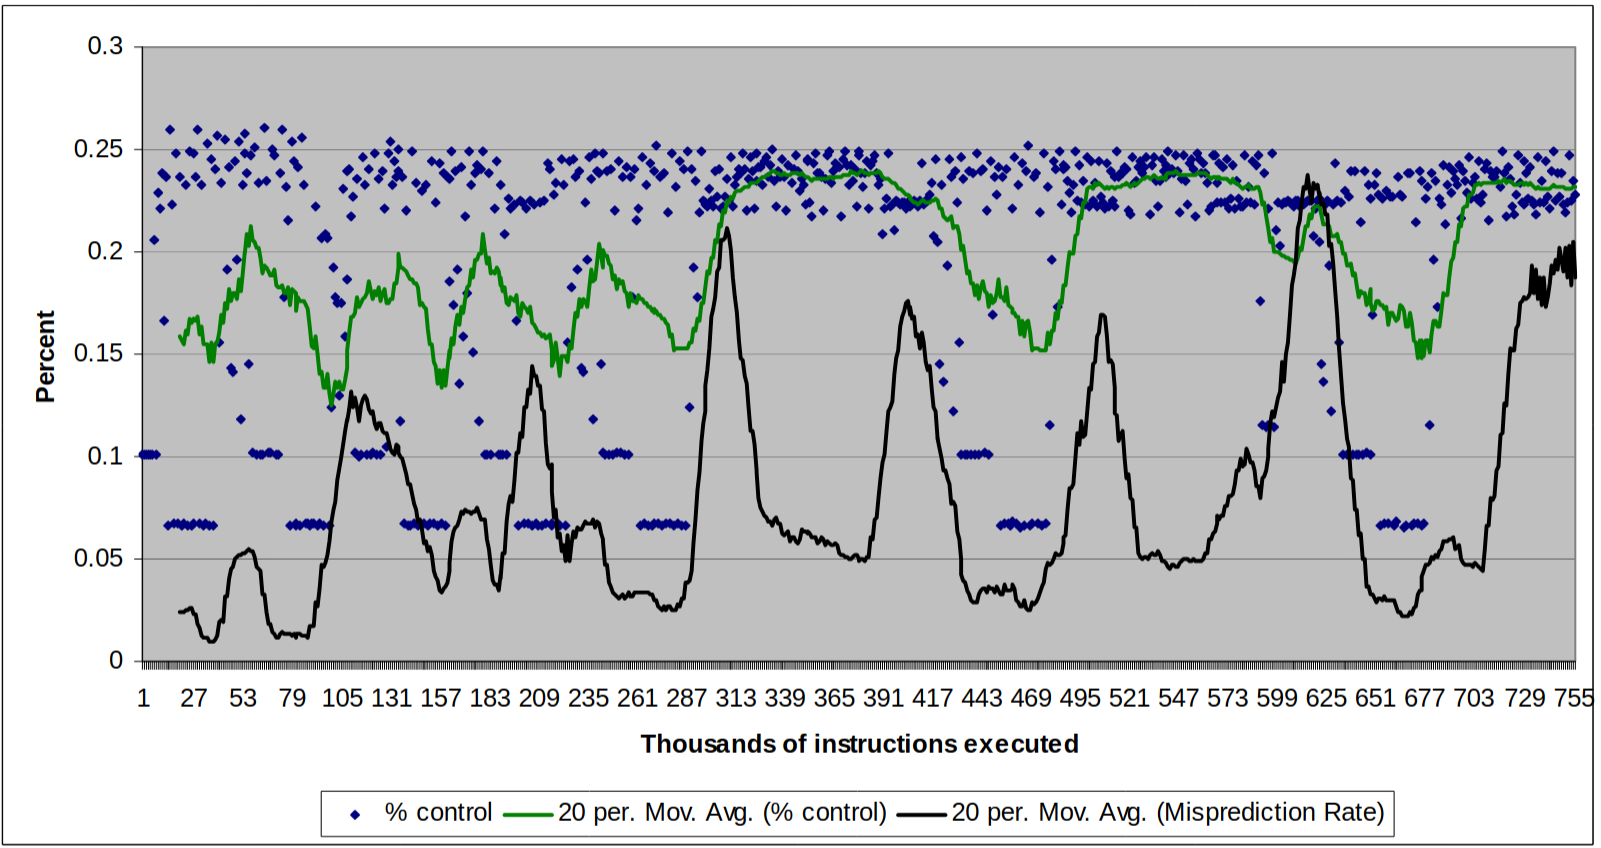
\includegraphics[width=15cm]{img/ST_Summer_Internship/coremark_control_instructions.png}
  \caption{Distribution of control instructions and mispredictions over CoreMark execution.}
  \label{fig:coremark_control}
\end{figure}

Overall CoreMark is well suited to comparing embedded processors. It is small, highly
portable, well understood, and highly controlled. CoreMark verifies that all computations
were completed correctly during execution, which helps debug any issues that may come
up. The run rules are clearly defined and reporting rules are enforced on the CoreMark
web site.
\section{C/C++ Build Process}
The construction of executable firmware for embedded systems necessitates interventions throughout the compilation toolchain, this requirement is driven by the absence of standardized hardware and resource constraints. Consequently, in our context, the build process is characterized by explicit configuration at each stage, including compiler optimizations, targeted assembly integration, and memory management via linker scripts.
\subsection{Compilation Toolchain}
\begin{figure}[H]
  \centering
  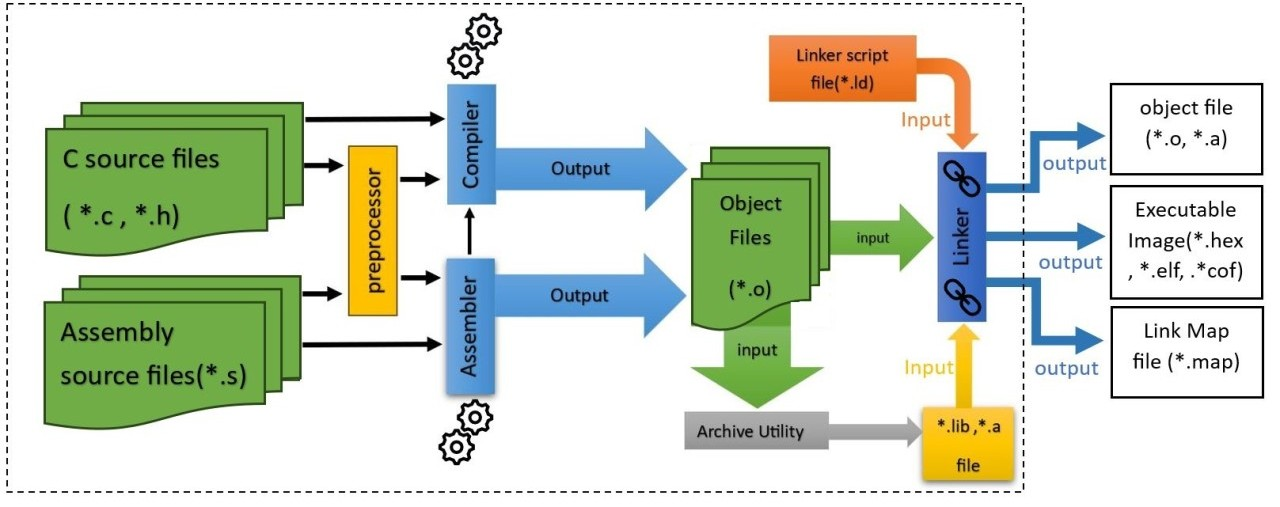
\includegraphics[width=15cm]{img/comp_diag.jpeg}
  \caption{Compilation Process Diagram}
  \label{fig:compilation}
\end{figure}
Going from source code in C/C++ to executable firmware involves multiple steps, in this subsection, we will go over them, highlighting the importance of each procedure.
\begin{itemize}
    \item \textbf{Preprocessor :} preprocessing is the first step of the build process, it expands macros and resolves defines as well as stripping comments from the code.
    \item \textbf{Assembler :} The assembler is the part of the toolchain that translates the high-level code into assembly code, which is the human-readable format of machine instruction, this step is done on a per-file basis.
    \item \textbf{Compiler :} Although the we use the term compilation as an equivalent to the whole process, compilation at its core is translating code into machine instructions, this step is what takes assembly mnemonics from each file and turns them into machine code also known as object files.
    \item \textbf{Linker :} The linking stage is the final and most important part of the process, since every c file is compiled separately into its own object file, they are not executable by default, the linker is what declares memory regions and associates symbols to the appropriate sections.
\end{itemize}
\subsection{Embedded Systems Toolchains}
While a standard toolchain for native development produces binaries that run directly on the host machine, an \textbf{embedded systems toolchain} targets a separate device with its own architecture, memory constraints, and hardware interfaces. 
This difference introduces several additional requirements beyond those of a regular host toolchain.

The most significant distinction is that an embedded toolchain must generate \textbf{cross-compiled code}. 
The compiler, assembler, and linker are configured to emit machine code compatible with the target processor's instruction set (e.g., ARM Cortex-M), rather than the host CPU. 
This involves selecting the correct ABI and handling architectural details such as endianness, hardware floating-point support, or specialized instruction extensions.
In addition to basic code generation, embedded toolchains typically include:
\begin{itemize}
	\item \textbf{Device-Specific Startup Code:} Since embedded systems do not run an operating system by default, the toolchain must provide initialization code that configures the processor state after reset. 
	This includes setting up the stack pointer, initializing memory sections, and defining the interrupt vector table.
	
	\item \textbf{Linker Scripts for Memory Mapping:} Unlike host systems where memory layout is abstracted by the operating system, embedded applications must explicitly define where code, data, and peripherals reside in memory. 
	The linker script enforces this mapping, ensuring that the binary fits within the device’s regions.
	
	\item \textbf{Runtime Support Libraries:} Embedded toolchains include specialized implementations of standard libraries designed to operate without an operating system. 
	These lightweight libraries provide essential functionality such as math operations or memory management while avoiding features that rely on system calls.
	
	\item \textbf{Debugging Interfaces:} Many embedded toolchains integrate support for hardware debugging through interfaces like SWD or JTAG. 
	This enables loading binaries onto the target, setting breakpoints, and inspecting registers or memory directly on the device.
	
	\item \textbf{Output Conversion Utilities:} Since microcontrollers typically require firmware images in raw binary or hex formats, embedded toolchains include utilities to convert the standard elf into target-specific formats such as Intel HEX or Motorola S-Record.
\end{itemize}

\subsection{Build Runners}
While small embedded projects can be compiled by invoking individual commands manually, this approach quickly becomes impractical as the codebase grows. 
Modern projects often contain hundreds of source files, complex dependencies, and different build configurations for debugging or optimization. 

A \textbf{build runner} (or build automation tool) automates this process by defining a set of rules that specify how source files should be transformed into the desired output.
At its core, a build runner:
\begin{itemize}
	\item Tracks dependencies between source files and generated files.
	\item Determines which parts of the project need to be rebuilt when a file changes.
	\item Invokes the appropriate compiler, assembler, or linker commands in the correct order.
\end{itemize}

Build runners operate based on explicit instructions provided through configuration files or scripts.
\subsection{Build Systems}
A \textbf{build system} is a higher-level abstraction built on top of build runners.
While a build runner executes rules, a build system focuses on generating and managing those rules for complex projects, often in a platform-agnostic way.

Build systems provide several key advantages:
\begin{itemize}
	\item \textbf{Portability:} They enable the same project to be built on different platforms or with different toolchains without rewriting build scripts.
	\item \textbf{Configuration Management:} They support multiple build configurations, such as debug or release builds, with different compiler flags and options.
	\item \textbf{Scalability:} They handle large projects with multiple modules, libraries, and external dependencies.
\end{itemize}

In practice, a build system generates low-level build instructions for a runner. 
For example, it may produce a set of dependency files and rules that a runner can execute efficiently. 
This separation of concerns allows developers to describe the project structure and relationships at a higher level, without directly managing every compiler or linker invocation.

In the context of embedded systems, build systems are particularly valuable because they can integrate device-specific settings, such as memory layouts or hardware abstraction layers, into the build process while remaining flexible enough to support multiple target devices and toolchains.

\section{Debugging}
Debugging embedded systems involves identifying and resolving issues that may occur in both hardware and software components. Unlike traditional software debugging, embedded debugging must account for real-time constraints, limited system visibility, and direct interaction with hardware peripherals. STM32 microcontrollers provide built-in debugging interfaces and features that greatly facilitate this process.

\subsection{Challenges of Embedded Debugging}
Embedded debugging presents unique challenges:
\begin{itemize}
	\item \textbf{Limited Visibility:} Unlike desktop systems, embedded devices lack standard output and comprehensive logging mechanisms, making it harder to inspect internal states.
	\item \textbf{Real-Time Behavior:} Debugging can disrupt timing-sensitive operations, potentially masking or introducing bugs.
	\item \textbf{Hardware Dependence:} Failures may stem from peripheral misconfiguration, incorrect clock settings, or external circuitry issues.
	\item \textbf{Resource Constraints:} Limited memory and processing power restrict the use of advanced debugging techniques.
\end{itemize}

\subsection{Debugging Interfaces and Tools}
In the case of STM32 devices, they integrate hardware support for debugging through two primary interfaces:
\begin{itemize}
	\item \textbf{SWD:} A two-pin protocol widely used for STM32 devices. It allows memory inspection, breakpoint handling, and peripheral monitoring with minimal I/O overhead.
	\item \textbf{JTAG:} A more comprehensive four-wire interface offering additional features such as boundary scan testing.
\end{itemize}
These interfaces are typically accessed via debug probes such as ST-LINK, J-Link, or CMSIS-DAP. They are supported by a wide range of IDEs and toolchains, including STM32CubeIDE, Keil µVision, and open-source solutions like OpenOCD and GDB.

\subsection{Core Debugging Techniques}
The following techniques are commonly used when debugging MCU applications:
\begin{itemize}
	\item \textbf{Breakpoints and Stepping:} Halt execution at specific lines to inspect variables and system state.
	\item \textbf{Watchpoints:} Trigger a halt when a specific memory location is read or written, useful for diagnosing memory corruption or stack overflows.
	\item \textbf{Peripheral Inspection:} Live monitoring of hardware registers to verify correct peripheral configuration.
	\item \textbf{Tracing:} Using the SWO pin to stream real-time events such as `printf`-style logs without blocking the CPU.
\end{itemize}

\subsection{Firmware-Based Debugging Aids}
Alongside hardware debuggers , simple firmware techniques can provide additional help in order to diagnose some issues:
\begin{itemize}
	\item \textbf{UART Logging:} Redirecting output to a UART peripheral for runtime logging. Though simple, it can introduce timing delays.
	\item \textbf{LED and GPIO Debugging:} Toggling pins to indicate execution flow or measure timing with an oscilloscope or logic analyzer.
	\item \textbf{Watchdog Management:} Pausing watchdog timers during debugging using the DBGMCU registers to prevent unintended resets.
\end{itemize}

\section{Open-CMSIS-Pack}
Software compatibility for component re-use has long been a challenge in the microcontroller space, which is much more diverse at the hardware level compared to PCs. Open-CMSIS-Pack removes this complexity, delivering a standard for software component packaging and related foundation tools for validation, distribution, integration, management, and maintenance.
\subsection{CMSIS-Packs} CMSIS-Packs are software components that contain device specific startup code, peripheral drivers, middleware, and board support packages. They provide a standardized delivery mechanism for software components and enable consistent project configuration across different development environments.
\begin{figure}[H]
	\centering
	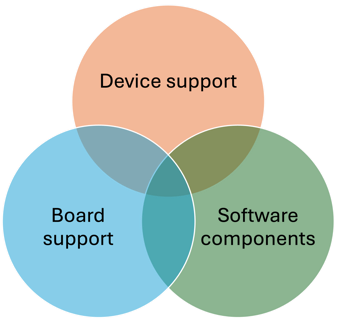
\includegraphics[height=10cm]{img/ST_Summer_Internship/pack_trinity.png}
	\caption{Software Packs Types}
	\label{fig:sw_trinity}
\end{figure}
\subsection{CMSIS-Pack Format}
The CMSIS-Pack format is used to deliver a software package and is aimed to be scalable for future requirements. It provides a management process and supports a tool independent distribution for:
\begin{itemize}
	\item \textbf{Device Support :}
	\begin{itemize}
		\item Information about the processor and it's features.
		\item C and assembly files for the device startup and access to the memory mapped peripheral registers.
		\item Parameters, technical information, and data sheets about the device family and the specific devices.
		\item Device description and available peripherals.
		\item Memory layout of internal and external RAM and ROM address ranges.
		\item Flash algorithms for programming the device.
		\item Debug and trace configurations as well as System View Description files for device specific display of the memory mapped peripheral registers. 
	\end{itemize}
	\item \textbf{Board Support :}
	\begin{itemize}
		\item Information about the development board and it's features.
		\item Parameters, technical information, and data sheets about the board, the mounted microcontroller, and peripheral devices.
		\item Drivers for on-board peripheral devices
	\end{itemize}
	\item \textbf{Software components :}
	\begin{itemize}
		\item A collection of source modules, header and configuration files as well as libraries.
		\item Documentation of the software, including features and APIs.
	\end{itemize}
\end{itemize}
\subsection{Software Components}
A software component encapsulates a set of related functions. They can contain C/C++ source files, object code, assembler files, header files, or libraries. The interfaces of software components should be defined with APIs to make them substitutable by other compatible components at design time.
CMSIS software components can also refer to multiple interfaces of other software components. This could be also a hardware abstraction layer for a device peripheral.
Configuration files contain application specific parameters for a software component. These files are typically copied to the user project workspace; all other files are not modified by the user and can remain in a separate location which avoids that a project workspace is polluted by many source files that should be considered as “black-box” elements by the application programmer.
\begin{figure}[H]
	\centering
	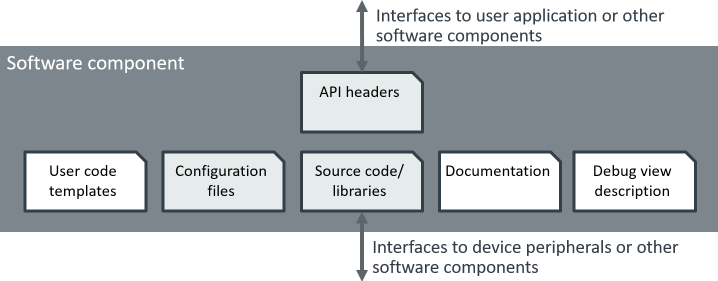
\includegraphics[width=15cm]{img/ST_Summer_Internship/software_component.png}
	\caption{Software Component Interface}
	\label{fig:sw_comp}
\end{figure}
\subsubsection{Component classification}
A component lists the files that belong to it and that are relevant for a project. The component itself or each individual file may refer to a condition that must resolve to true; if it is false, the component or file is not applicable in the given context.

Each software component must have the following attributes that are used to identify the component:
\begin{itemize}
	\item \textbf{Component Class (Cclass):} A component class which is a top-level component name, for example CMSIS, Device, File System
	\item \textbf{Component Group (Cgroup):} A component group name, for example CMSIS:RTOS, Device:Startup, File System:CORE
	\item \textbf{Component Version (Cversion):} the version number of the software component.
\end{itemize}



\subsection{CMSIS Solution Project Structure}
As an effort to standardize the embedded software ecosystem, the csolution(CMSIS Solution) project structure came into place, it is a set of configuration files that is meant to describe your overall application, from the workspace, to projects, software layers and default configurations.
This approach allows the user to centralize all the configuration of an application.
\begin{figure}[H]
	\centering
	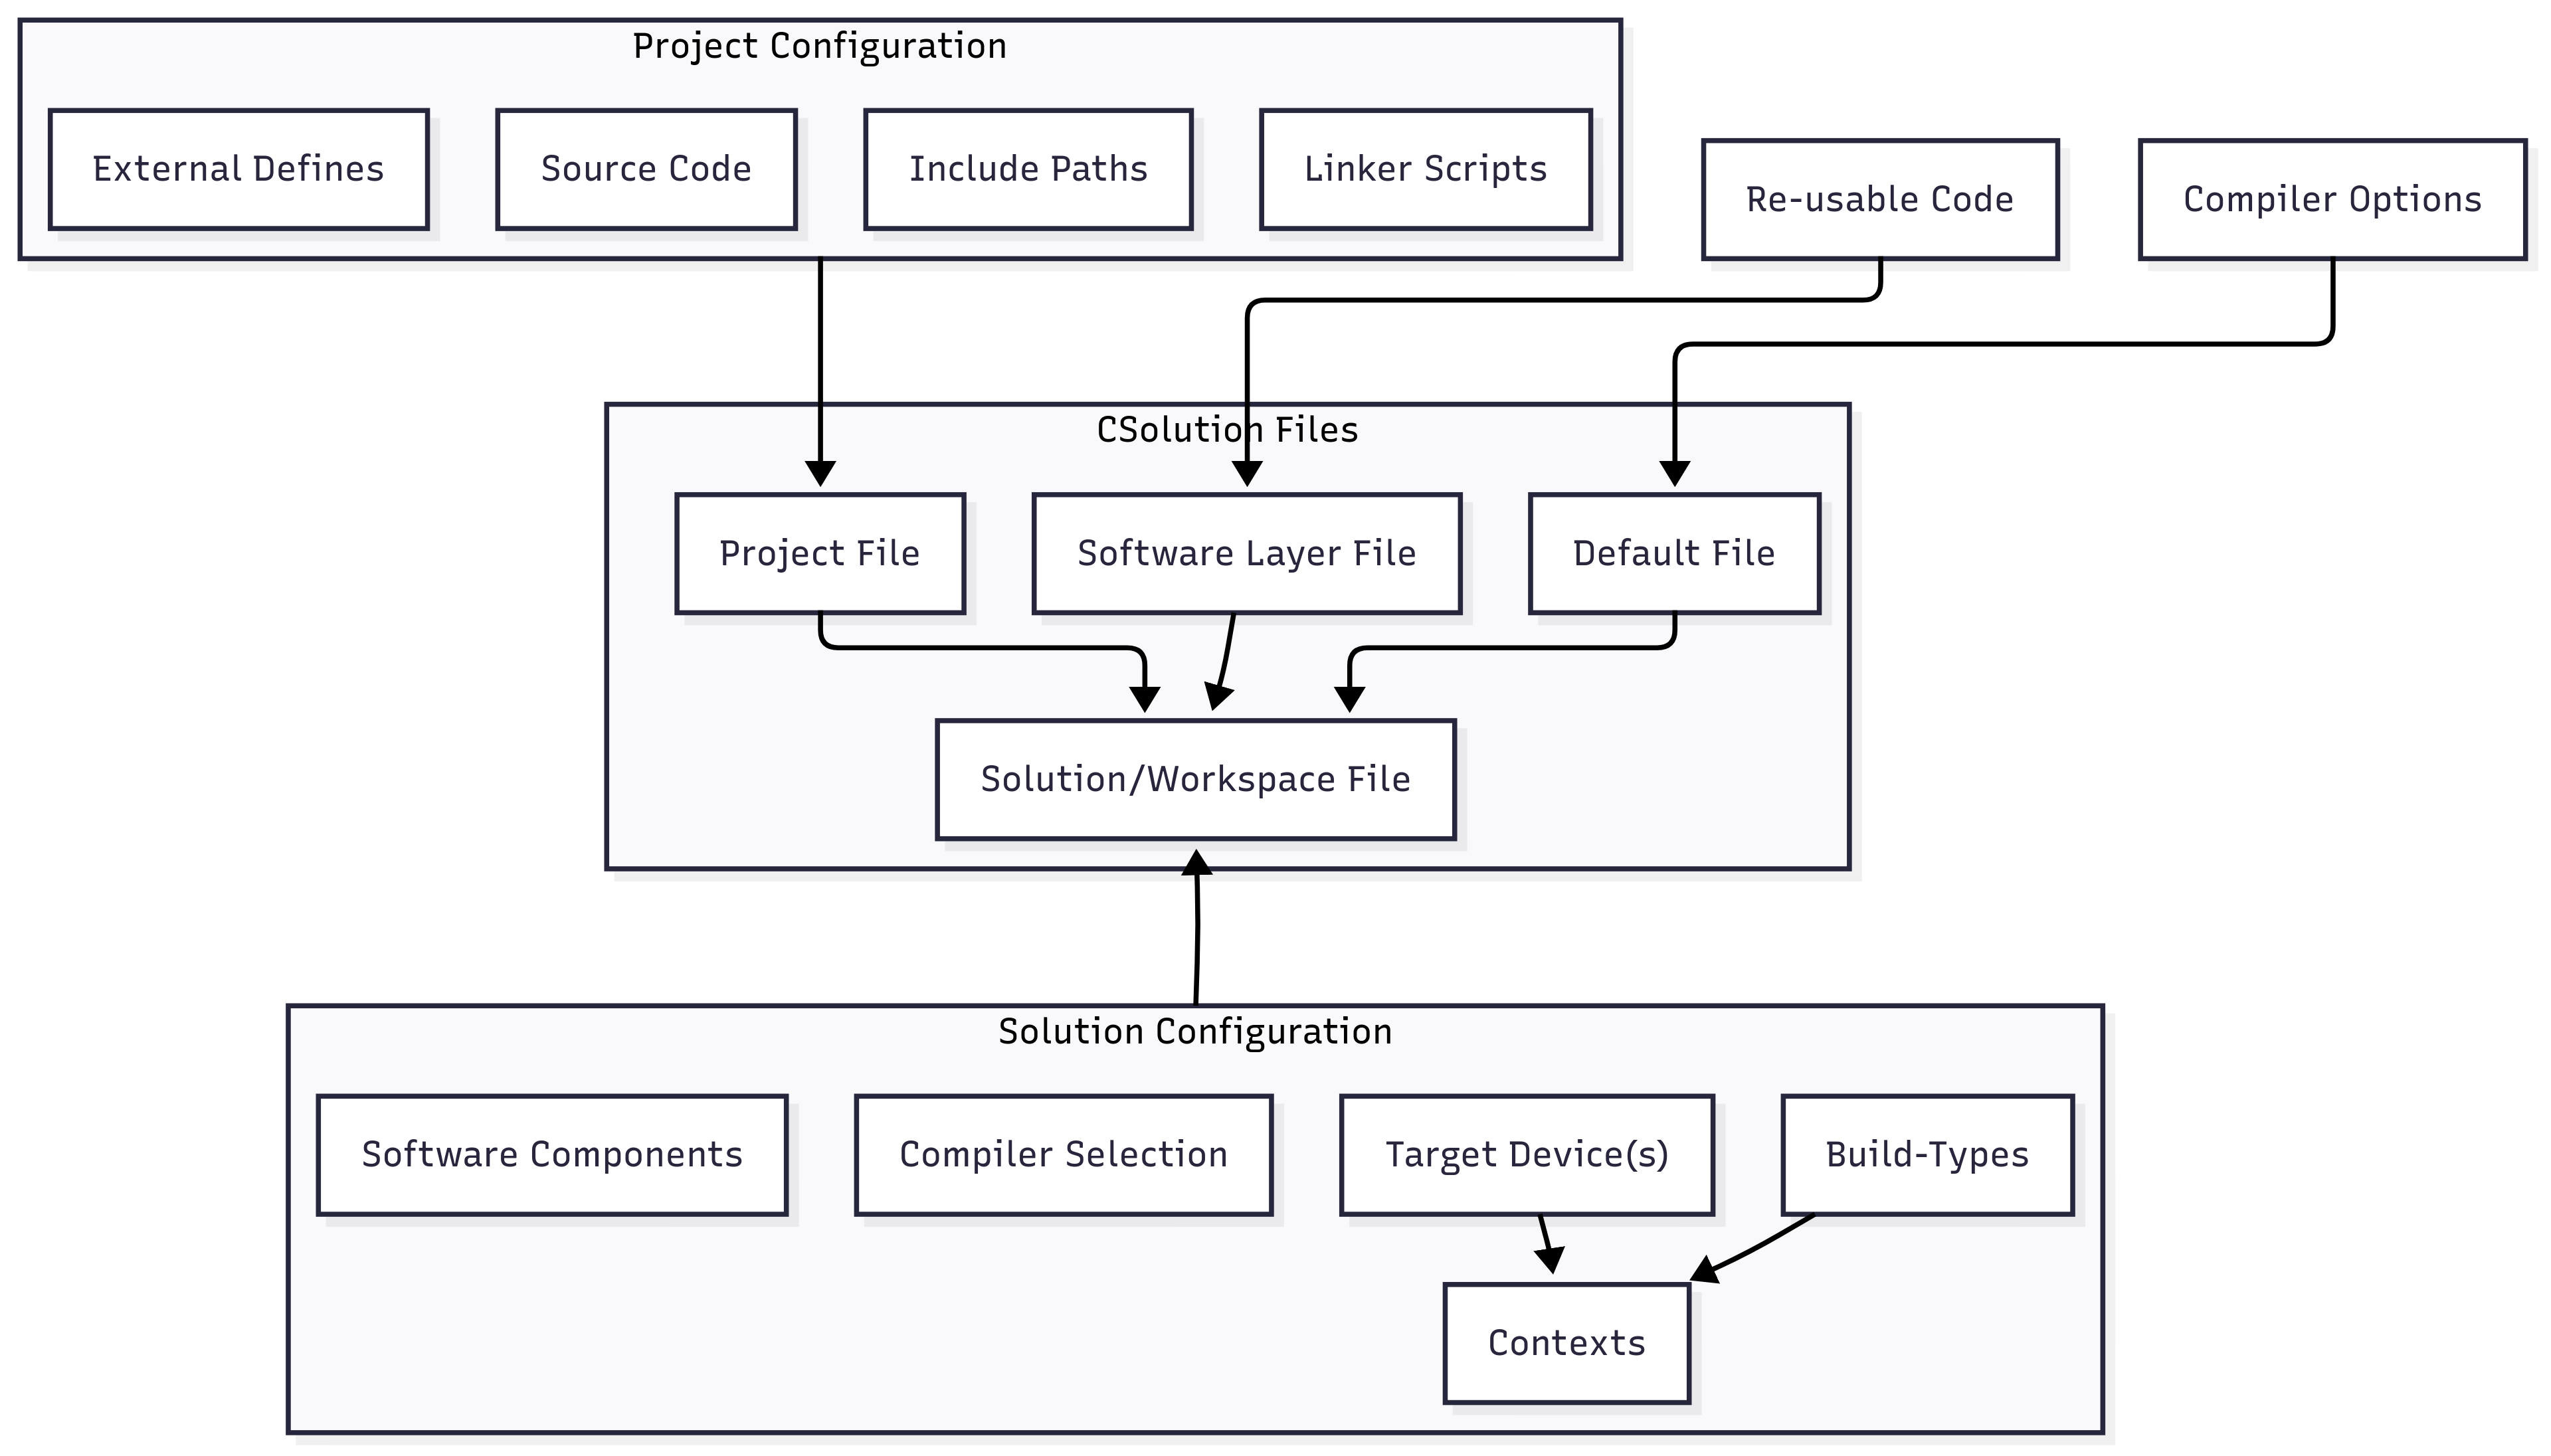
\includegraphics[width=15cm]{./img/ST_Summer_Internship/csolution_project_structure.png}
	\caption{CMSIS Solution Project Structure}
	\label{fig:csln_files}
\end{figure}  
\subsubsection{CMSIS solution files}
The CMSIS-Toolbox gets its information from the csolution project files, these are YAML configuration files used to describe the application's context:
\begin{itemize}
	\item \textbf{Solution file} A solution is the software view of the complete system. It combines projects that can be generated independently and therefore, manages related projects. It also specifies the targeted device(s) and build type(s). The file has the format *.csolution.yml.
	\item \textbf{Project file} The *.cproject.yml file has the content of a single independent build step, it specifies the source files to compile, sets the include directories and the necessary defines.
	\item \textbf{Layer file} Software layers collect source files and software components along with configuration files for reuse in different projects. Software Layers gives projects a better structure and simplifies:
	\begin{itemize}
		\item Development flows with evaluation boards and production hardware.
		\item Evaluation of middleware and hardware modules across different microcontroller boards.
		\item Code reuse across projects, i.e. board support for test-case deployment.
		\item Test-driven software development on simulation model and hardware.
	\end{itemize}
	\item \textbf{Default Configuration file} The cdefault.yml file contains a common set of compiler-specific settings that select reasonable defaults with miscellaneous controls for each compiler. 
\end{itemize}

\section{Project Generation}
When trying to run benchmarks across a wide variety of MCUs, the project structure follows the same pattern, and the dependencies can be expressed in a logical way relating to the device's metadata, therefore, automating the process will prove handy.
There are multiple techniques to be used to generate a fully working project from scratch.
\subsection{Regular Expressions:}
    The phrase regular expressions, or regexes, is often used to mean the specific, standard textual syntax for representing patterns for matching text. Each character in a regular expression (that is, each character in the string describing its pattern) is either a metacharacter, having a special meaning, or a regular character that has a literal meaning.
    A regular expression, often called a pattern, specifies a set of strings required for a particular purpose. 
\subsubsection{Operations}
Most formalisms provide the following operations to construct regular expressions. 
\begin{itemize}
    \item \textbf{Boolean "OR":} A vertical bar separates alternatives. For example, gray|grey can match "gray" or "grey".
    \item \textbf{Grouping} Parentheses are used to define the scope and precedence of the operators (among other uses). For example, gray|grey and gr(a|e)y are equivalent patterns which both describe the set of "gray" or "grey".
    \item \textbf{Quantification} A quantifier after an element (such as a token, character, or group) specifies how many times the preceding element is allowed to repeat.
    The available quantifications are:
    \begin{itemize}
        \item \textbf{Zero or One:} Denoted by the question mark \textbf{"?"} symbol.
        \item \textbf{Zero or More:} Denoted by the asterisk \textbf{"*"} (derived from the Kleene star). 
        \item \textbf{One or More:} Denoted by the plus symbol \textbf{"+"}.
        \item \textbf{N or More:} Denoted by the expression : \textbf{"\{N, \}"} where N is a positive integer.
        \item \textbf{N or Less:} Denoted by the expression : \textbf{"\{ ,N\}"} where N is a positive integer.
        \item \textbf{Between N and M times:} Denoted by the expression: \textbf{"\{N, M\}"} where N and M are positive integers such that N < M.
    \end{itemize}
    \item \textbf{Wildcard:} Denoted by the dot \textbf{"."} it matches any single character
\end{itemize}
These operations can be combined interchangeably to create complex expressions to describe the desired system.
\subsubsection{IEEE POSIX Standard}
The IEEE POSIX standard has three sets of compliance: BRE (Basic Regular Expressions), ERE (Extended Regular Expressions), and SRE (Simple Regular Expressions). SRE is deprecated, in favor of BRE, as both provide backward compatibility.
BRE and ERE work together. ERE adds ?, +, and |, and it removes the need to escape the metacharacters ( ) and \{ \}, which are required in BRE. Furthermore, as long as the POSIX standard syntax for regexes is adhered to, there can be, and often is, additional syntax to serve specific (yet POSIX compliant) applications. Although POSIX.2 leaves some implementation specifics undefined, BRE and ERE provide a "standard" which has since been adopted as the default syntax of many tools, where the choice of BRE or ERE modes is usually a supported option.
Perl regexes have become a de facto standard, having a rich and powerful set of atomic expressions. Perl has no "basic" or "extended" levels. As in POSIX EREs, ( ) and \{ \} are treated as metacharacters unless escaped; other metacharacters are known to be literal or symbolic based on context alone. Additional functionality includes lazy matching, backreferences, named capture groups, and recursive patterns.

\subsection{Templates \& File Manipulation}
File generation templates are pre-defined structures or blueprints used to create new files with standardized content and formatting.
\subsubsection{Template Definition}
A template file is created containing boilerplate text, placeholders for dynamic content (variables), and sometimes logic for conditional generation.
\subsubsection{Parameterization}
The template defines parameters that can be filled in by the user or a program when generating a new file. These parameters can be single-valued, arrays or maps containing relevant information.
\subsubsection{Template Execution}
When a new file is needed, the template is selected, and the required parameters are provided. A generation engine then processes the template, replacing placeholders with the provided values and executing any embedded logic to produce the final file.
\begin{figure}[H]
	\centering
	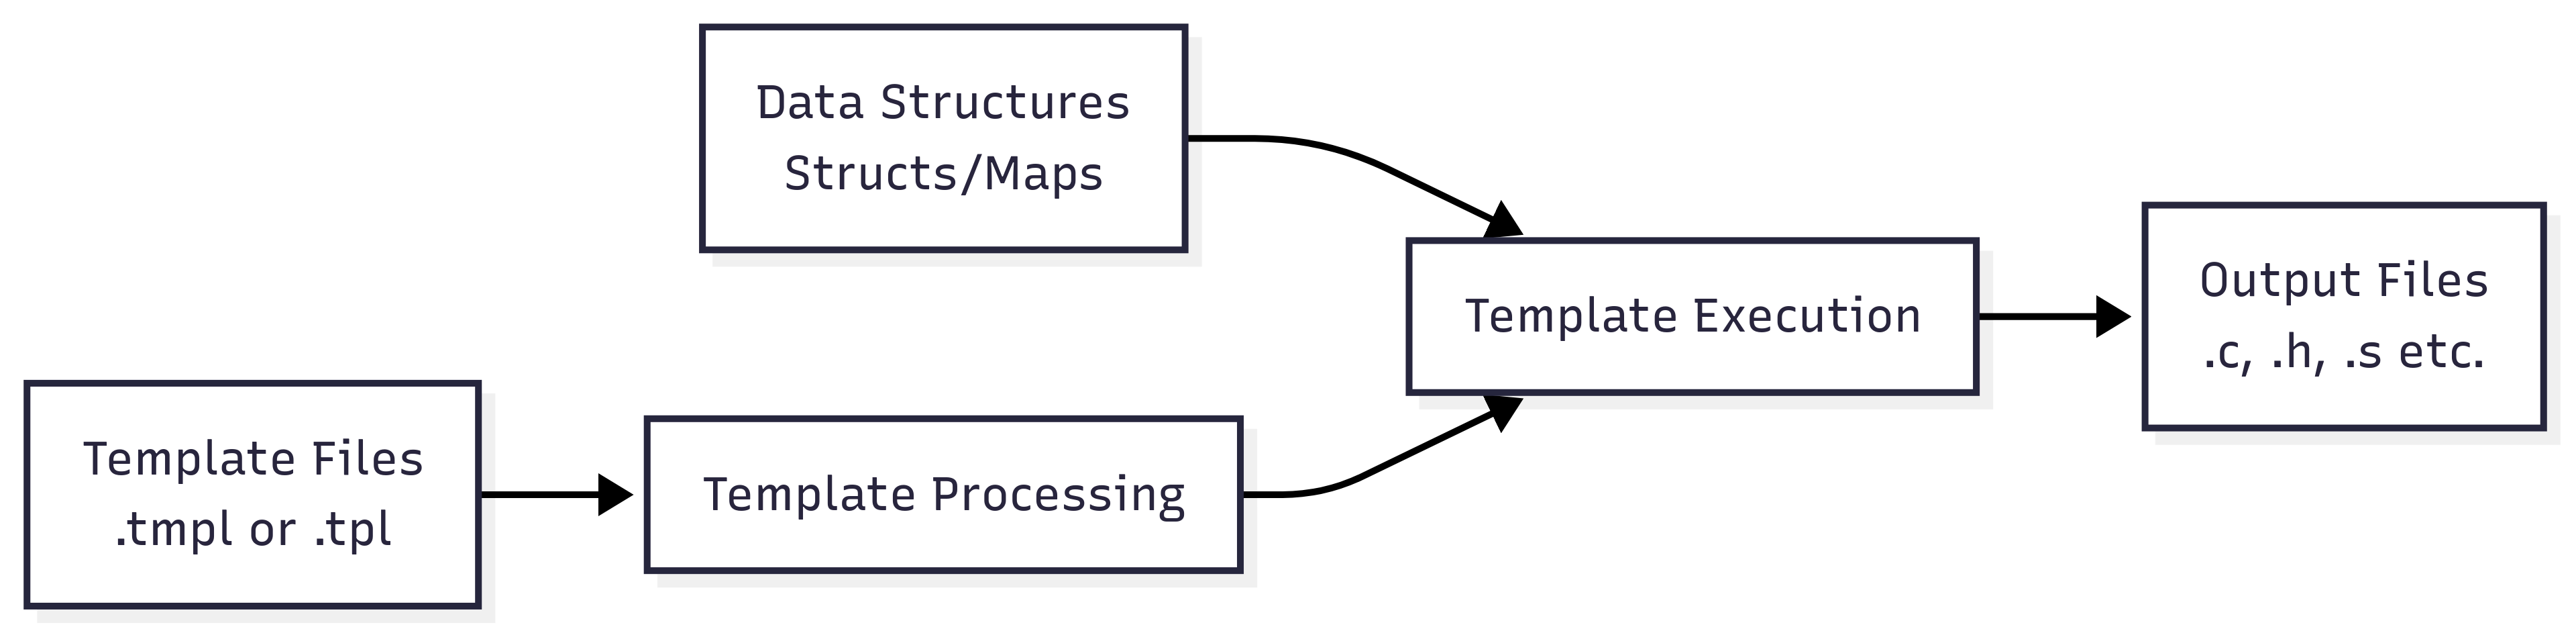
\includegraphics[width=15cm]{img/ST_Summer_Internship/template_workflow.png}
	\caption{Templating Process}
	\label{fig:tempalte_proc}
\end{figure}

\subsection{CMSIS-Toolbox Generators}
Generators, such as STM32CubeMX or MCUXpresso Config Tools, simplify the configuration for devices and boards. The CMSIS-Toolbox implements a generic interface for generators. They may be used to:
\begin{itemize}
	\item Configure device and/or board settings, such as clock configuration or pinout.
	\item Add and configure software drivers, for example, for UART, SPI, or I/O ports.
	\item Configure parameters of an algorithm, such as DSP filter design or motor control parameters.
\end{itemize}
\subsubsection{Generator Integration (STM32CubeMX Example)}
\begin{figure}[H]
	\centering
	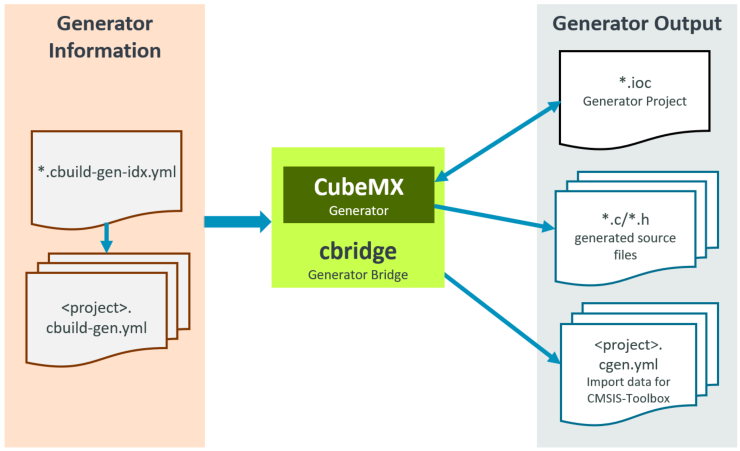
\includegraphics[width=15cm]{img/Generator-Integration.png}
	\caption{Generator Integration in CMSIS-Toolbox}
	\label{fig:generator}
\end{figure}
The Figure \ref{fig:generator} shows how the STM32CubeMX generator is integrated into the CMSIS build process. The data flow is exemplified on STM32CubeMX (Generator ID for this example is CubeMX). The information about the project is delivered to the generator using the Generator Information files (<solution-name>.cbuild-gen-idx.yml and <context>.cbuild-gen.yml). This information provides CubeMX with the project context, such as the selected board or device, and CPU mode, such as TrustZone, disabled/enabled.
The utility cbridge gets as parameter the <solution-name>.cbuild-gen-idx.yml and calls the generator. For the CubeMX generator example, these files are created:
\begin{itemize}
	\item *.ioc CubeMX project file with current project settings
	\item *.c/.h source files, i.e. for interfacing with drivers
	\item <project-name>.cgen.yml (created by cbridge) provides the data for project import into the csolution build process.
\end{itemize}
\newpage


\section*{Conclusion}
This chapter has provided an overview of the key theoretical concepts and technologies relevant to the project. We began by exploring the STM32 microcontroller ecosystem, including the various series and ARM Cortex-M cores that form the foundation of these devices. The STM32Cube firmware package was introduced as a comprehensive software suite for STM32 development.

We then examined the principles of benchmarking, with a particular focus on the CoreMark benchmark and its application to microcontrollers. The C/C++ build process for embedded systems was detailed, highlighting the unique requirements and toolchains needed for cross-compilation.

The chapter also covered debugging techniques specific to embedded systems, outlining both hardware interfaces like SWD and JTAG, as well as firmware-based approaches. The Open-CMSIS-Pack standard was presented as a solution for software component packaging and project configuration in the microcontroller space.

Finally, we discussed methods for automating project generation, including the use of regular expressions, file templates, and specialized tools like the CMSIS-Toolbox generators. These concepts and tools form the theoretical and practical basis for the work conducted during this internship, setting the stage for the implementation and results that will be presented in subsequent chapters.

        \clearpage
        
       \chapter{Objectives Specification and Work Environment}

\section*{Introduction}
This chapter will first define the project's functional and non-functional requirements, then we will discuss the chosen cryptographic algorithms, explaining the reasoning behind their selection and offering an overview of how each algorithm works. Finally we will specify the hardware and software resources necessary for this demonstration. 

\section{Project Specification}
Requirements analysis is a fundamental phase in every project realization process. It is based on the study of the project's features as well as the constraints. In this section, we will cover both the functional and non-functional requirements.

\subsection{Functional Requirements}

The goal of the "CryptoEngine" demo is to establish secure communication between an STM32XX MCU using "CryptoEngine" and an STM32U5 MCU using PKA and AES. Secure communication means guaranteeing the three key security concepts: confidentiality, integrity, and authenticity.

\begin{itemize}
    \item \textbf{Confidentiality:} Ensuring that only authorized parties can understand the messages exchanged. This is achieved through:
    \begin{itemize}
        \item \textbf{Asymmetric Key Management:} Implement asymmetric key  management for ECDSA and ECDH keys, ensuring secure storage and handling of private keys and generation of public keys.
        \item \textbf{Shared Secret Computation:} Compute the ECDH shared secret using the exchanged public keys, which will be used as the basis for deriving symmetric encryption keys.
    \end{itemize}
    
    \item \textbf{Integrity:} Ensuring that the message has not been altered during transmission. This is achieved through:
    \begin{itemize}
       \item \textbf{Symmetric Message Encryption and Decryption:} Use AES GCM symmetric encryption to encrypt messages and verify their integrity during transmission. This also serves as an authentication check.
    \end{itemize}
    
    \item \textbf{Authenticity:} Ensuring that the communicating parties are who they claim to be. This is achieved through:
    \begin{itemize}
        \item \textbf{Signature Generation and Verification:} Enable the generation and verification of digital signatures using ECDSA to ensure the authenticity of the communicating parties.
    \end{itemize}
\end{itemize}

Establishing a secure, authenticated encryption system using modern cryptographic standards, including Elliptic Curve Digital Signature Algorithm (ECDSA) for digital signatures, Elliptic Curve Diffie-Hellman (ECDH) for key exchange, and Advanced Encryption Standard Galois Counter Mode (AES GCM) for encryption and authentication, is the primary goal.

Table \ref{tab:functional_requirements} neatly summarizes the functional requirements for our demonstration.

\setlength{\tabcolsep}{10pt} % Adjust the padding
\renewcommand{\arraystretch}{1.5} % Adjust the row height

\begin{table}[h]
\centering
\caption{Functional Requirements for Secure Communication}
\label{tab:functional_requirements}
\begin{tabular}{|m{2.5cm}|p{3.5cm}|p{9cm}|}
\hline
\textbf{Security Requirement} & \textbf{Component} & \textbf{Description} \\ \hline
\multirow{2}{*}{Confidentiality} & Key Management & Implement key management for ECDSA and ECDH keys, ensuring
secure storage and handling of private keys and generation of public keys. \\ \cline{2-3} 
 & Shared Secret Computation & Compute the ECDH shared secret using the exchanged public keys, which will be used as the basis for deriving symmetric encryption keys. \\ \hline
Integrity & Message Encryption and Decryption & Use AES GCM to encrypt messages and verify their integrity during transmission. This also serves as an additional authenticity verification. \\ \hline
Authenticity & Signature Generation and Verification & Enable the generation and verification of digital signatures using ECDSA to ensure the authenticity of the communicating parties. \\ \hline
\end{tabular}
\end{table}

\subsection{Non-Functional Requirements}
Below are the non-functional requirements or the constraints that the functional expectations must abide by:
\begin{itemize}
    \item \textbf{Clarity:} The demo should be clear and easily understandable, enabling users without extensive technical expertise to grasp the concepts.
     \item \textbf{Transferability:} The knowledge and experience gained from the demo should empower users to apply cryptographic techniques in their own projects with ease.
   \item \textbf{Modularity:} The demo should be designed in a modular way, allowing individual components to be easily reused or adapted for different applications.
  \item \textbf{Feature Comparison:} The demo should highlight the new features and enhancements introduced by the "CryptoEngine" compared to its predecessors, demonstrating the improvements in security and usability.
\end{itemize}

\section{Cryptographic Decisions and Context}
Before delving further into the implementation details, it is crucial to understand the rationale behind the cryptographic algorithms and protocols chosen for this demo. This section elucidates the reasons for selecting specific cryptographic methods and their relevance to the project's objectives.

\subsection{Elliptic Curve Diffie-Hellman}
Elliptic Curve Diffie-Hellman (ECDH) is a widely adopted key exchange protocol that facilitates secure and efficient key exchange between parties. We opted for ECDH due to its significant advantages over traditional algorithms like RSA, particularly in resource-constrained environments.

\begin{itemize}
    \item \textbf{Resource Efficiency:} ECDH is less resource-intensive compared to RSA, making it suitable for embedded systems with limited computational power and memory.
     \item \textbf{Optimal Key Size:} A 256-bit key size strikes a balance between security and performance, making it suitable for embedded applications, including our demo.
    
\end{itemize}

\begin{figure}[H]
    \centering
    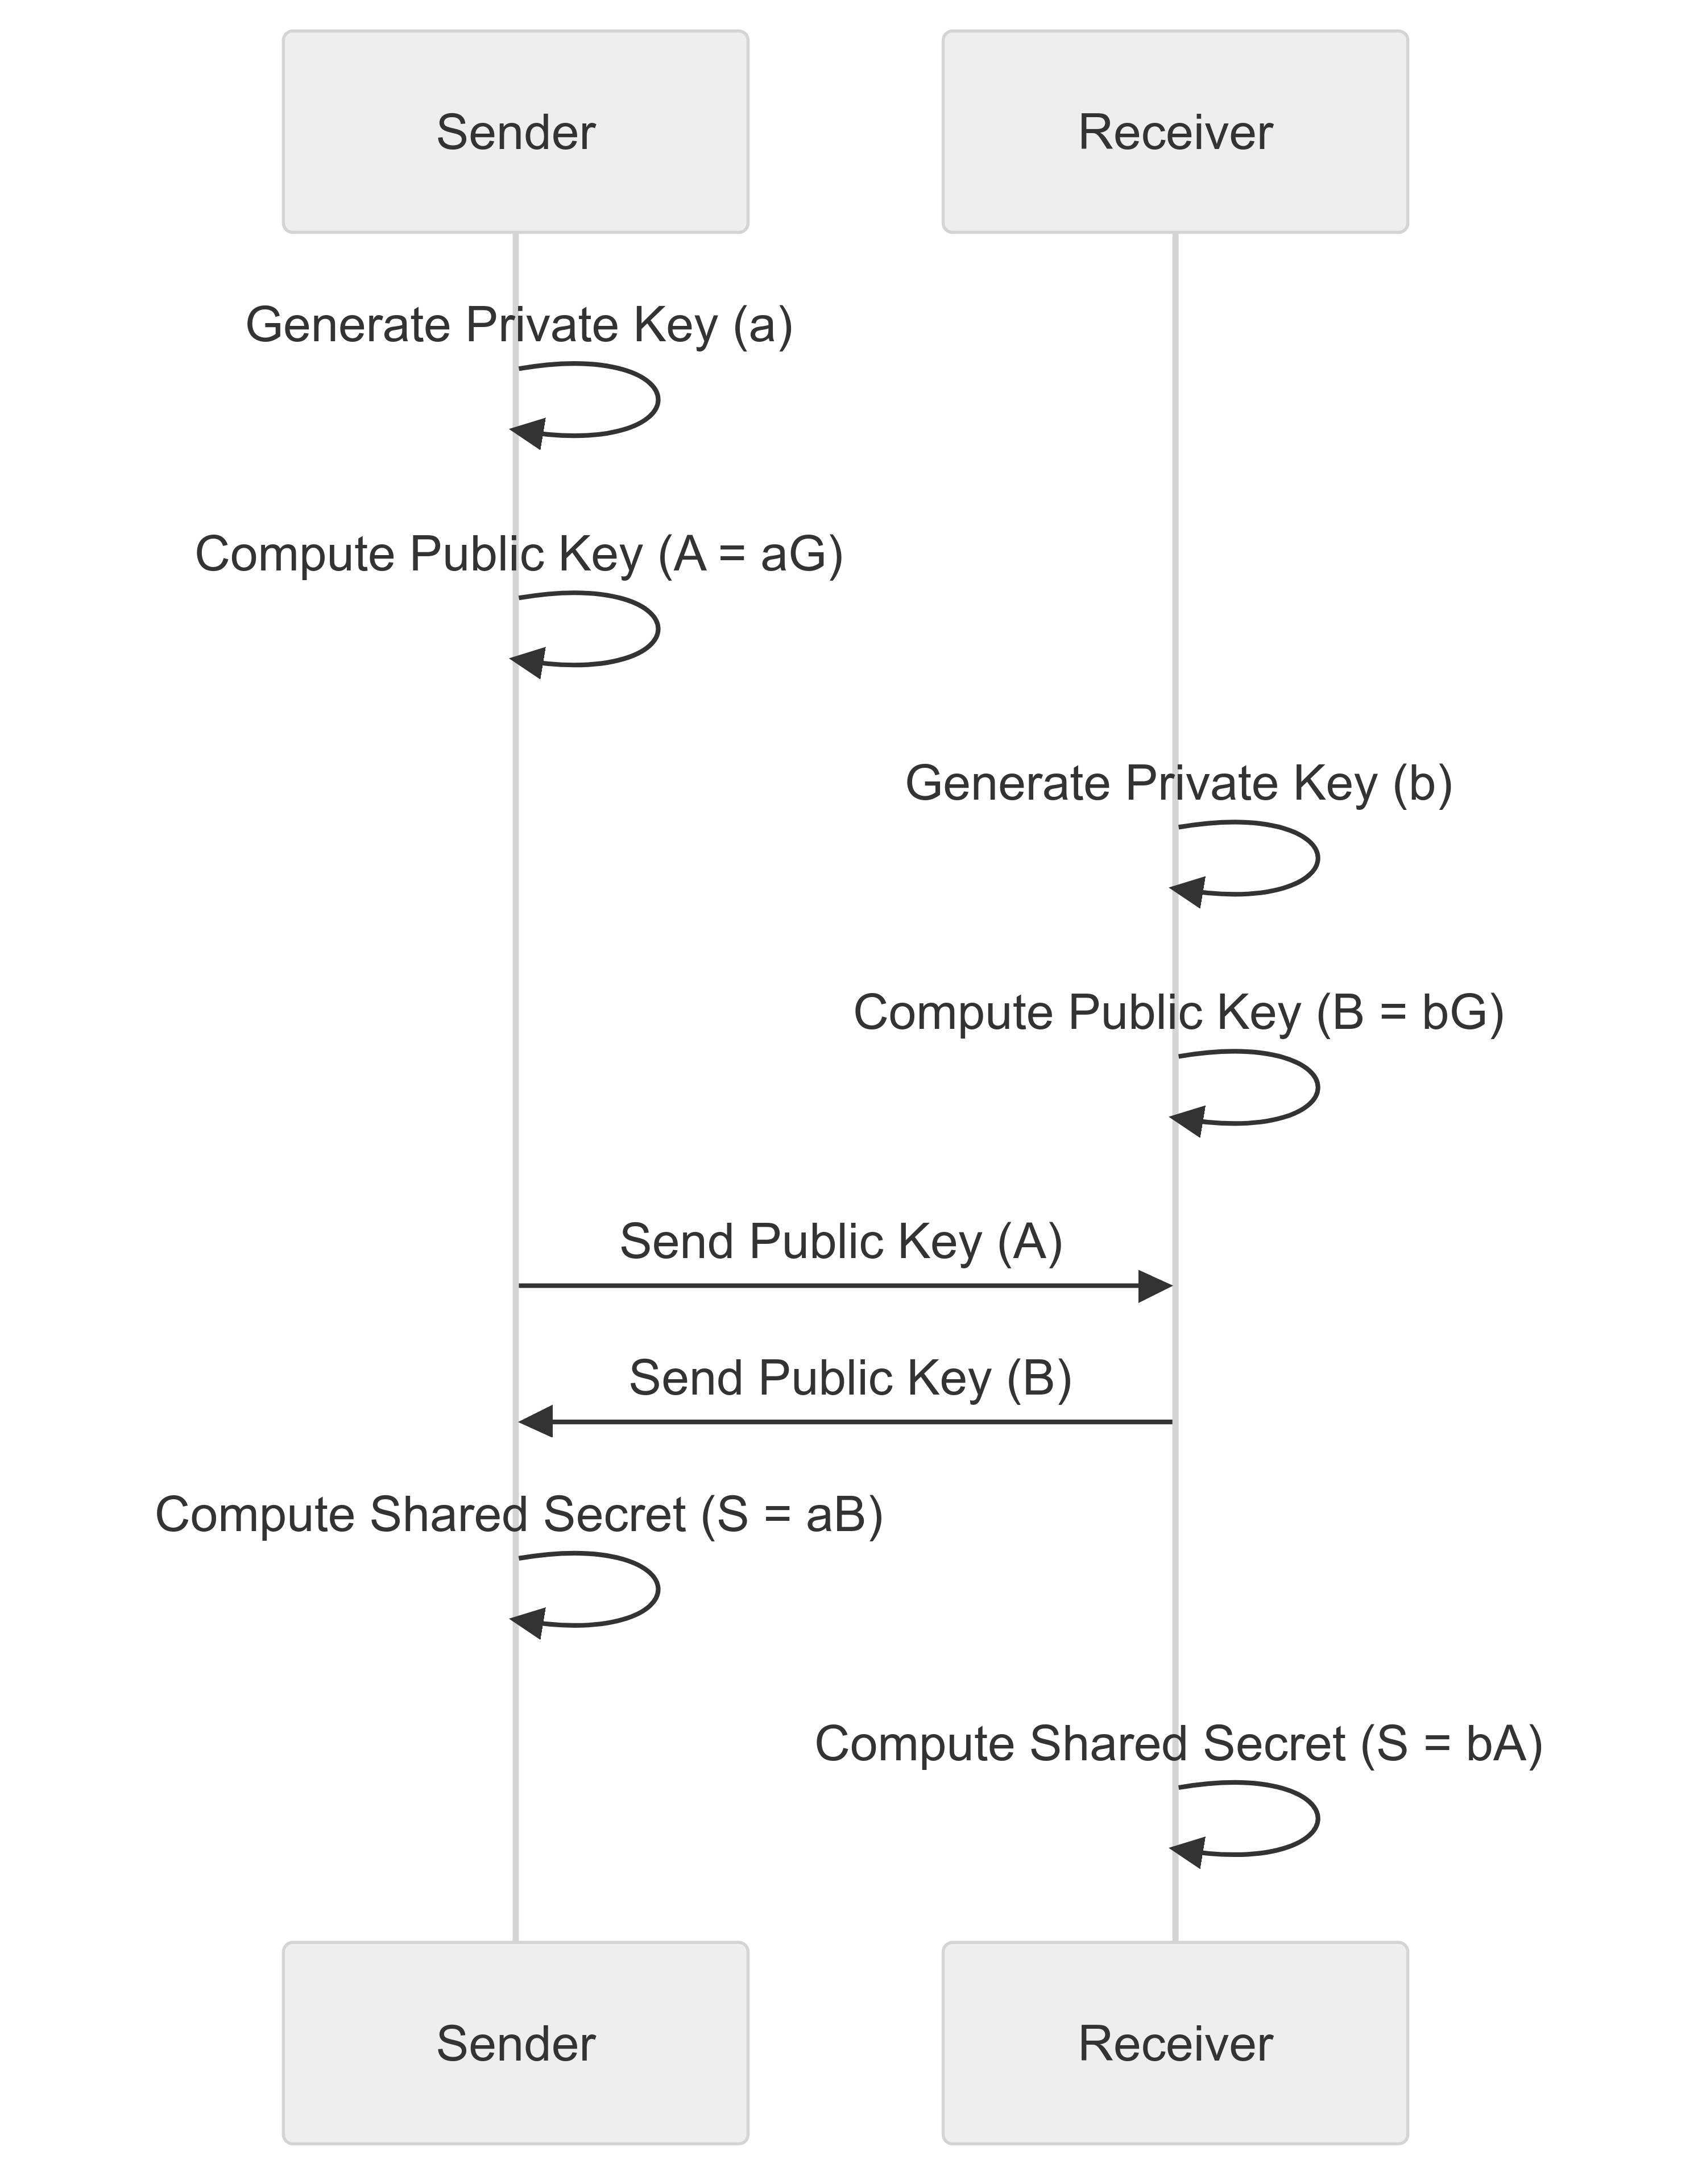
\includegraphics[width=10cm]{img/ECDH.png}
    \caption{Elliptic Curve Diffie Hellman Process}
    \label{fig:ecdh_graph}
\end{figure} 

The ECDH process as shown in Figure \ref{fig:ecdh_graph}, begins with both the sender and the receiver independently generating their own private and public key pairs.

The sender generates a private key \(a\) and computes their corresponding public key \(A = aG\), where \(G\) is a predefined generator point on the elliptic curve. Similarly, the receiver generates a private key \(b\) and computes their corresponding public key \(B = bG\).

Once the key pairs are generated, the sender and receiver exchange their public keys over the insecure channel. The sender sends their public key \(A\) to the receiver, and the receiver sends their public key \(B\) to the sender. Despite the exchange occurring over an insecure channel, the private keys \(a\) and \(b\) remain confidential and are never transmitted.

After receiving the public key from the other party, each participant computes the shared secret using their own private key and the received public key. The sender calculates the shared secret \(S = aB\) by multiplying their private key \(a\) with the receiver's public key \(B\). Conversely, the receiver calculates the shared secret \(S = bA\) by multiplying their private key \(b\) with the sender's public key \(A\). Due to the properties of elliptic curves, both computations result in the same shared secret \(S\), which can be used to derive a symmetric key for encrypting and decrypting subsequent communications.



\subsection{Elliptic Curve Digital Signature Algorithm}
The Elliptic Curve Digital Signature Algorithm (ECDSA) is a renowned digital signature algorithm that enables the generation and verification of digital signatures, ensuring data authenticity and integrity.

\begin{itemize}
    \item \textbf{Efficiency:} ECDSA is highly efficient, offering faster computations and smaller key sizes compared to other digital signature algorithms like RSA.
    \item \textbf{Compatibility:} ECDSA is supported by the PKA (Public Key Accelerator) peripheral in STM32 products, making it an ideal choice for our demo.
    \item \textbf{Security:} ECDSA provides strong security guarantees, leveraging the hardness of the elliptic curve discrete logarithm problem.
\end{itemize}

The graph in Figure \ref{fig:ecdsa_graph} illustrates a typical digital signature process that applies to many algorithms, including ECDSA. It involves two main phases: signing by the sender and verification by the receiver. 

On the sender side, the process begins with key generation, where a pair of keys—a private key and a public key—are created. The sender then prepares a message that needs to be signed. This message is passed through a hashing algorithm to produce a message hash, ensuring that the message is represented in a fixed-size format. The private key and the message hash are then input into the signing algorithm to generate a signature. Subsequently, the message, signature, and public key are transmitted to the receiver.

On the receiver side, the verification algorithm uses the public key, message hash, and signature to verify the authenticity of the message. The receiver independently generates the message hash using the same hashing algorithm as the sender. If the signature is valid, the sender is authenticated, providing confidence that the message has not been tampered with and is from the legitimate sender. Conversely, if the signature is invalid, the sender is not authenticated, indicating potential tampering or an illegitimate sender. This process ensures both the integrity and authenticity of the message, making digital signatures a necessity for secure communications.

\begin{figure}[H]
    \centering
    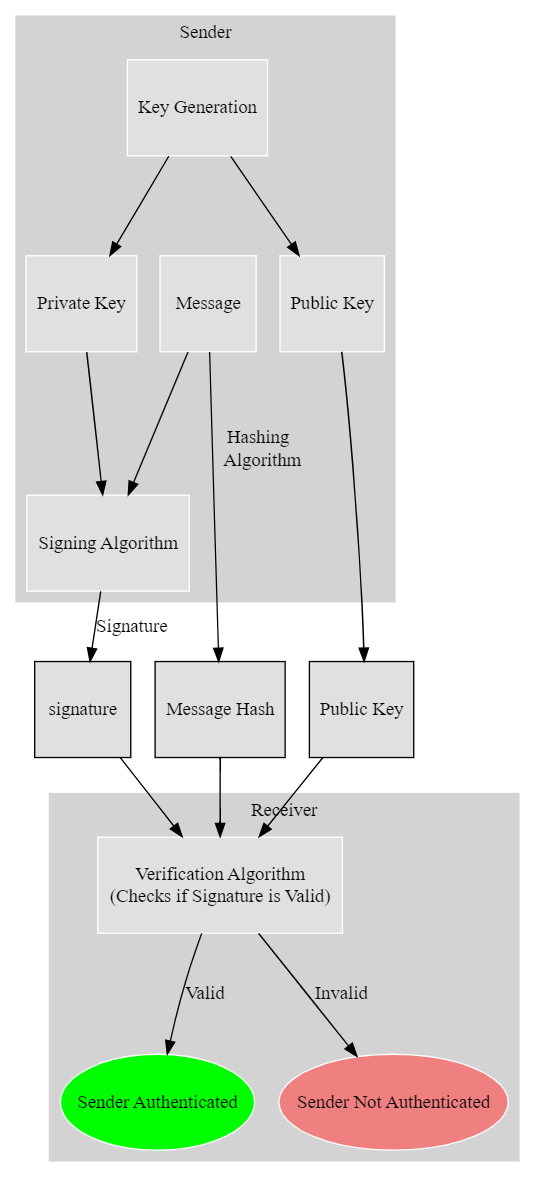
\includegraphics[width=7.5cm]{img/TD ECDSA Graph.png}
    \caption{Typical Digital Signature Process}
    \label{fig:ecdsa_graph}
\end{figure}


\subsection{NIST P-256 Curve}
\label{curve_param}
For this demo, we have chosen the NIST P-256 curve for both the ECDSA algorithm and the ECDH protocol. This decision was based on several factors:

\begin{itemize}
    \item \textbf{NIST Recommendation:} The P-256 curve is recommended by the National Institute of Standards and Technology (NIST) for its security and efficiency \cite{nist_p256}.
    \item \textbf{Popularity:} The P-256 curve is widely used and well-supported across various cryptographic libraries and tools, facilitating interoperability and ease of use \cite{Telemetry}.
    \item \textbf{Documentation:} Extensive documentation and implementation examples are available for the P-256 curve, simplifying the development and debugging processes.
    \item \textbf{Smaller Key Size:} ECDH achieves the same security level as RSA with much smaller key sizes. For instance, a 256-bit key in ECDH provides equivalent security to a 3072-bit key in RSA, as illustrated in Table \ref{tab:rsa_vs_ecc}.
   
    
\end{itemize}
\begin{table}[H]
    \caption{Comparison of Key Sizes and Security Levels between RSA and ECC}
    \centering
    \begin{tabular}{|c|c|c|}
        \hline
        \textbf{Algorithm} & \textbf{Key Size (bits)} & \textbf{Security Level (bits)} \\
        \hline
      
        RSA & 2048 & 112 \\
        \hline
        RSA & 3072 & 128 \\
        \hline
        RSA & 15360 & 256 \\
        \hline
        ECC (P-224) & 224 & 112 \\
        \hline
        ECC (P-256) & 256 & 128 \\
        \hline
        ECC (P-521) & 521 & 256 \\
        \hline
    \end{tabular}

    \label{tab:rsa_vs_ecc}
\end{table}
\textit{Note: Using a 256-bit curve means that private keys will be 256 bits long, and our public key's x and y coordinates will each be 256 bits long, totaling 512-bit size for the public keys.}


\subsection{AES Galois Counter Mode}
AES Galois Counter Mode (GCM) is a robust symmetric encryption algorithm that provides both confidentiality and integrity. We chose AES GCM for the following reasons:

\begin{itemize}
    \item \textbf{High Security:} AES GCM offers strong security guarantees, making it resistant to various cryptographic attacks. It is widely regarded as one of the most secure modes of operation for AES.
    \item \textbf{Integrity and Authenticity:} AES GCM generates an authentication tag during encryption, which can be used to verify the integrity and authenticity of the encrypted data. This dual functionality is particularly valuable in ensuring data security.
    \item \textbf{Standardization:} AES GCM is a standardized encryption mode, widely adopted in various security protocols and applications, ensuring compatibility and interoperability.
\end{itemize}
Figure \ref{fig:aes_gcm} \cite{U5_Refman} illustrates the AES GCM process.
It begins with the initialization vector being fed into a counter. The counter's value, along with the symmetric encryption key, is used by the AES encryption function to generate a series of encrypted blocks. These encrypted blocks are then XORed with the corresponding plaintext blocks to produce the ciphertext.

Simultaneously, the encrypted blocks are processed through a Galois field multiplication (GF2mul), which contributes to generating an authentication tag (TAG) for integrity verification. The output of the AES GCM process is both the encrypted message (ciphertext) and the authentication tag, ensuring confidentiality and integrity of the data. The diagram also shows the handling of additional blocks and the finalization step to complete the authentication process.

\begin{figure}[H]
  \centering
  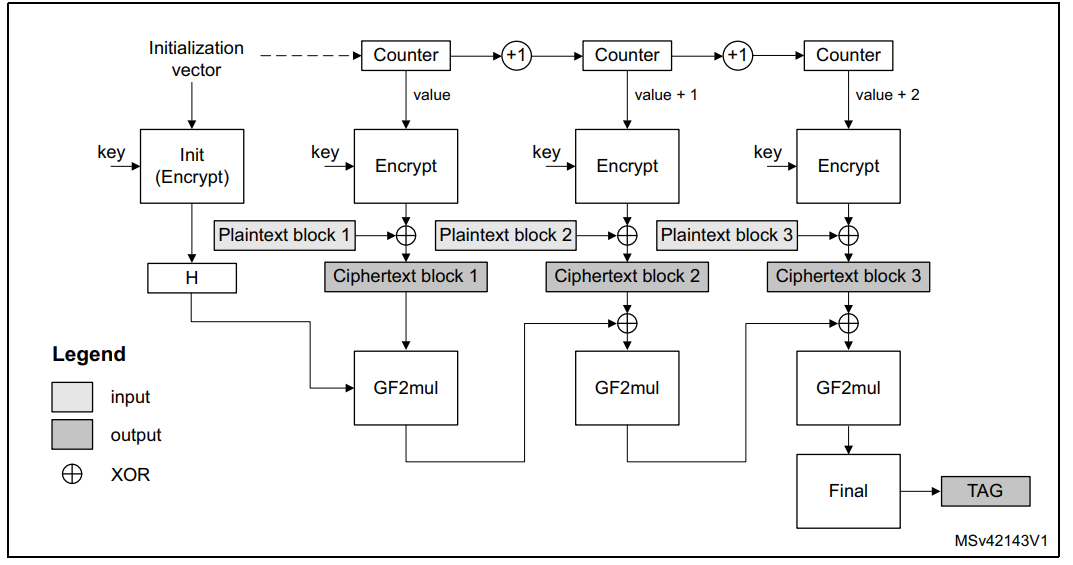
\includegraphics[width=17cm]{img/AES GCM.png}
  \caption{AES Galois Counter Mode Process }
  \label{fig:aes_gcm}
\end{figure}

\section{Use-Case Diagram}
\begin{figure}[H]
  \centering
  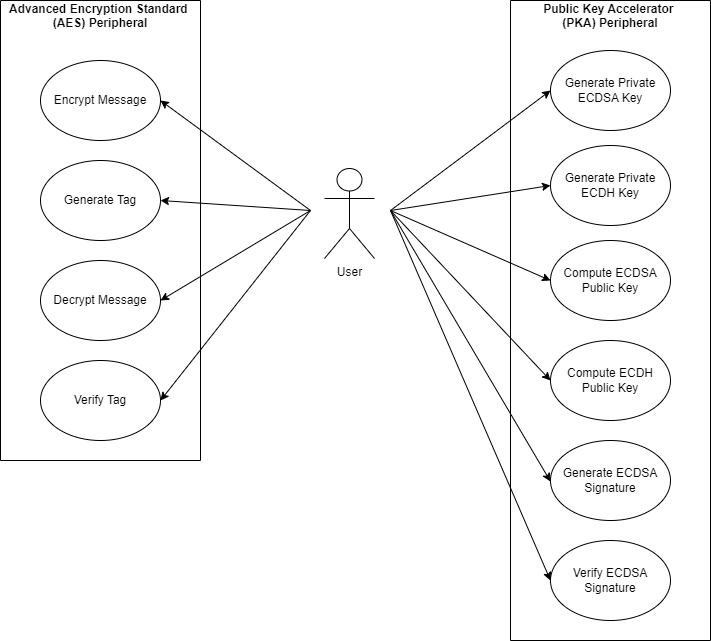
\includegraphics[width=14.5cm]{img/use case 2.png}
  \caption{Use-Case Diagram for Cryptographic Peripherals (AES and PKA)}
  \label{fig:use_case_diagram}
\end{figure}

The Use-Case diagram in Figure \ref{fig:use_case_diagram} illustrates the interactions between a user and the cryptographic peripherals available on STM32 MCUs.
 Refer to Table \ref{tab:use_cases} for an in-depth explanation:

\begin{longtable}{|p{5cm}|p{6cm}|p{4cm}|}
\caption{Use Cases for Cryptographic Peripherals} \label{tab:use_cases} \\

\hline
\textbf{Use Case} & \textbf{Relevance} & \textbf{Peripheral Used} \\ \hline
\endfirsthead

\multicolumn{3}{c}%
{{\bfseries \tablename\ \thetable{} -- continued from previous page}} \\
\hline
\textbf{Use Case} & \textbf{Relevance} & \textbf{Peripheral Used} \\ \hline
\endhead

\hline \multicolumn{3}{|r|}{{Continued on next page}} \\ \hline
\endfoot

\hline
\endlastfoot

Generate Private ECDSA Key & Part of the key management process, ensuring secure storage and handling of private keys, which contributes to confidentiality. & PKA (Public Key Accelerator) \\ \hline
Generate Private ECDH Key & Part of the key management process and essential for establishing a shared secret, contributing to confidentiality. & PKA (Public Key Accelerator) \\ \hline
Compute ECDSA Public Key & Necessary for signature verification, which ensures authenticity. & PKA (Public Key Accelerator) \\ \hline
Compute ECDH Public Key & Necessary for the ECDH key exchange process, contributing to confidentiality. & PKA (Public Key Accelerator) \\ \hline
Generate ECDSA Signature & Ensures the authenticity of the communicating parties by providing a way to verify identities. & PKA (Public Key Accelerator) \\ \hline
Verify ECDSA Signature & Ensures the authenticity of the communicating parties by verifying the provided signatures. & PKA (Public Key Accelerator) \\ \hline
Encrypt Message & Ensures confidentiality and integrity of the message during transmission. & AES (Advanced Encryption Standard) \\ \hline
Generate Tag & Ensures the integrity of the message and also serves as an authentication check. & AES (Advanced Encryption Standard) \\ \hline
Decrypt Message & Ensures confidentiality and integrity of the message during transmission. & AES (Advanced Encryption Standard) \\ \hline
Verify Tag & Ensures the integrity of the message and also serves as an authentication check. & AES (Advanced Encryption Standard) \\ \hline

\end{longtable}






\section{Work Environment}
In this section, we outline the hardware and software resources utilized during the internship project that were essential for the development, testing, and demonstration of the "CryptoEngine" peripheral.

\subsection{Hardware Resources}
\begin{itemize}
    \item \textbf{STM32XX MCU:} The STM32XX microcontroller unit (MCU) is the primary hardware platform used for implementing and testing the "CryptoEngine" peripheral. The STM32XX series offers advanced cryptographic features and peripherals, making it ideal for secure communication applications.
    \item \textbf{STM32U545 MCU:} The STM32U545 microcontroller unit is used for comparison and interoperability with the STM32XX MCU. This board utilizes the AES and PKA peripherals to perform cryptographic operations, enabling secure key exchange and encryption.
    \begin{figure}[H]
  \centering
  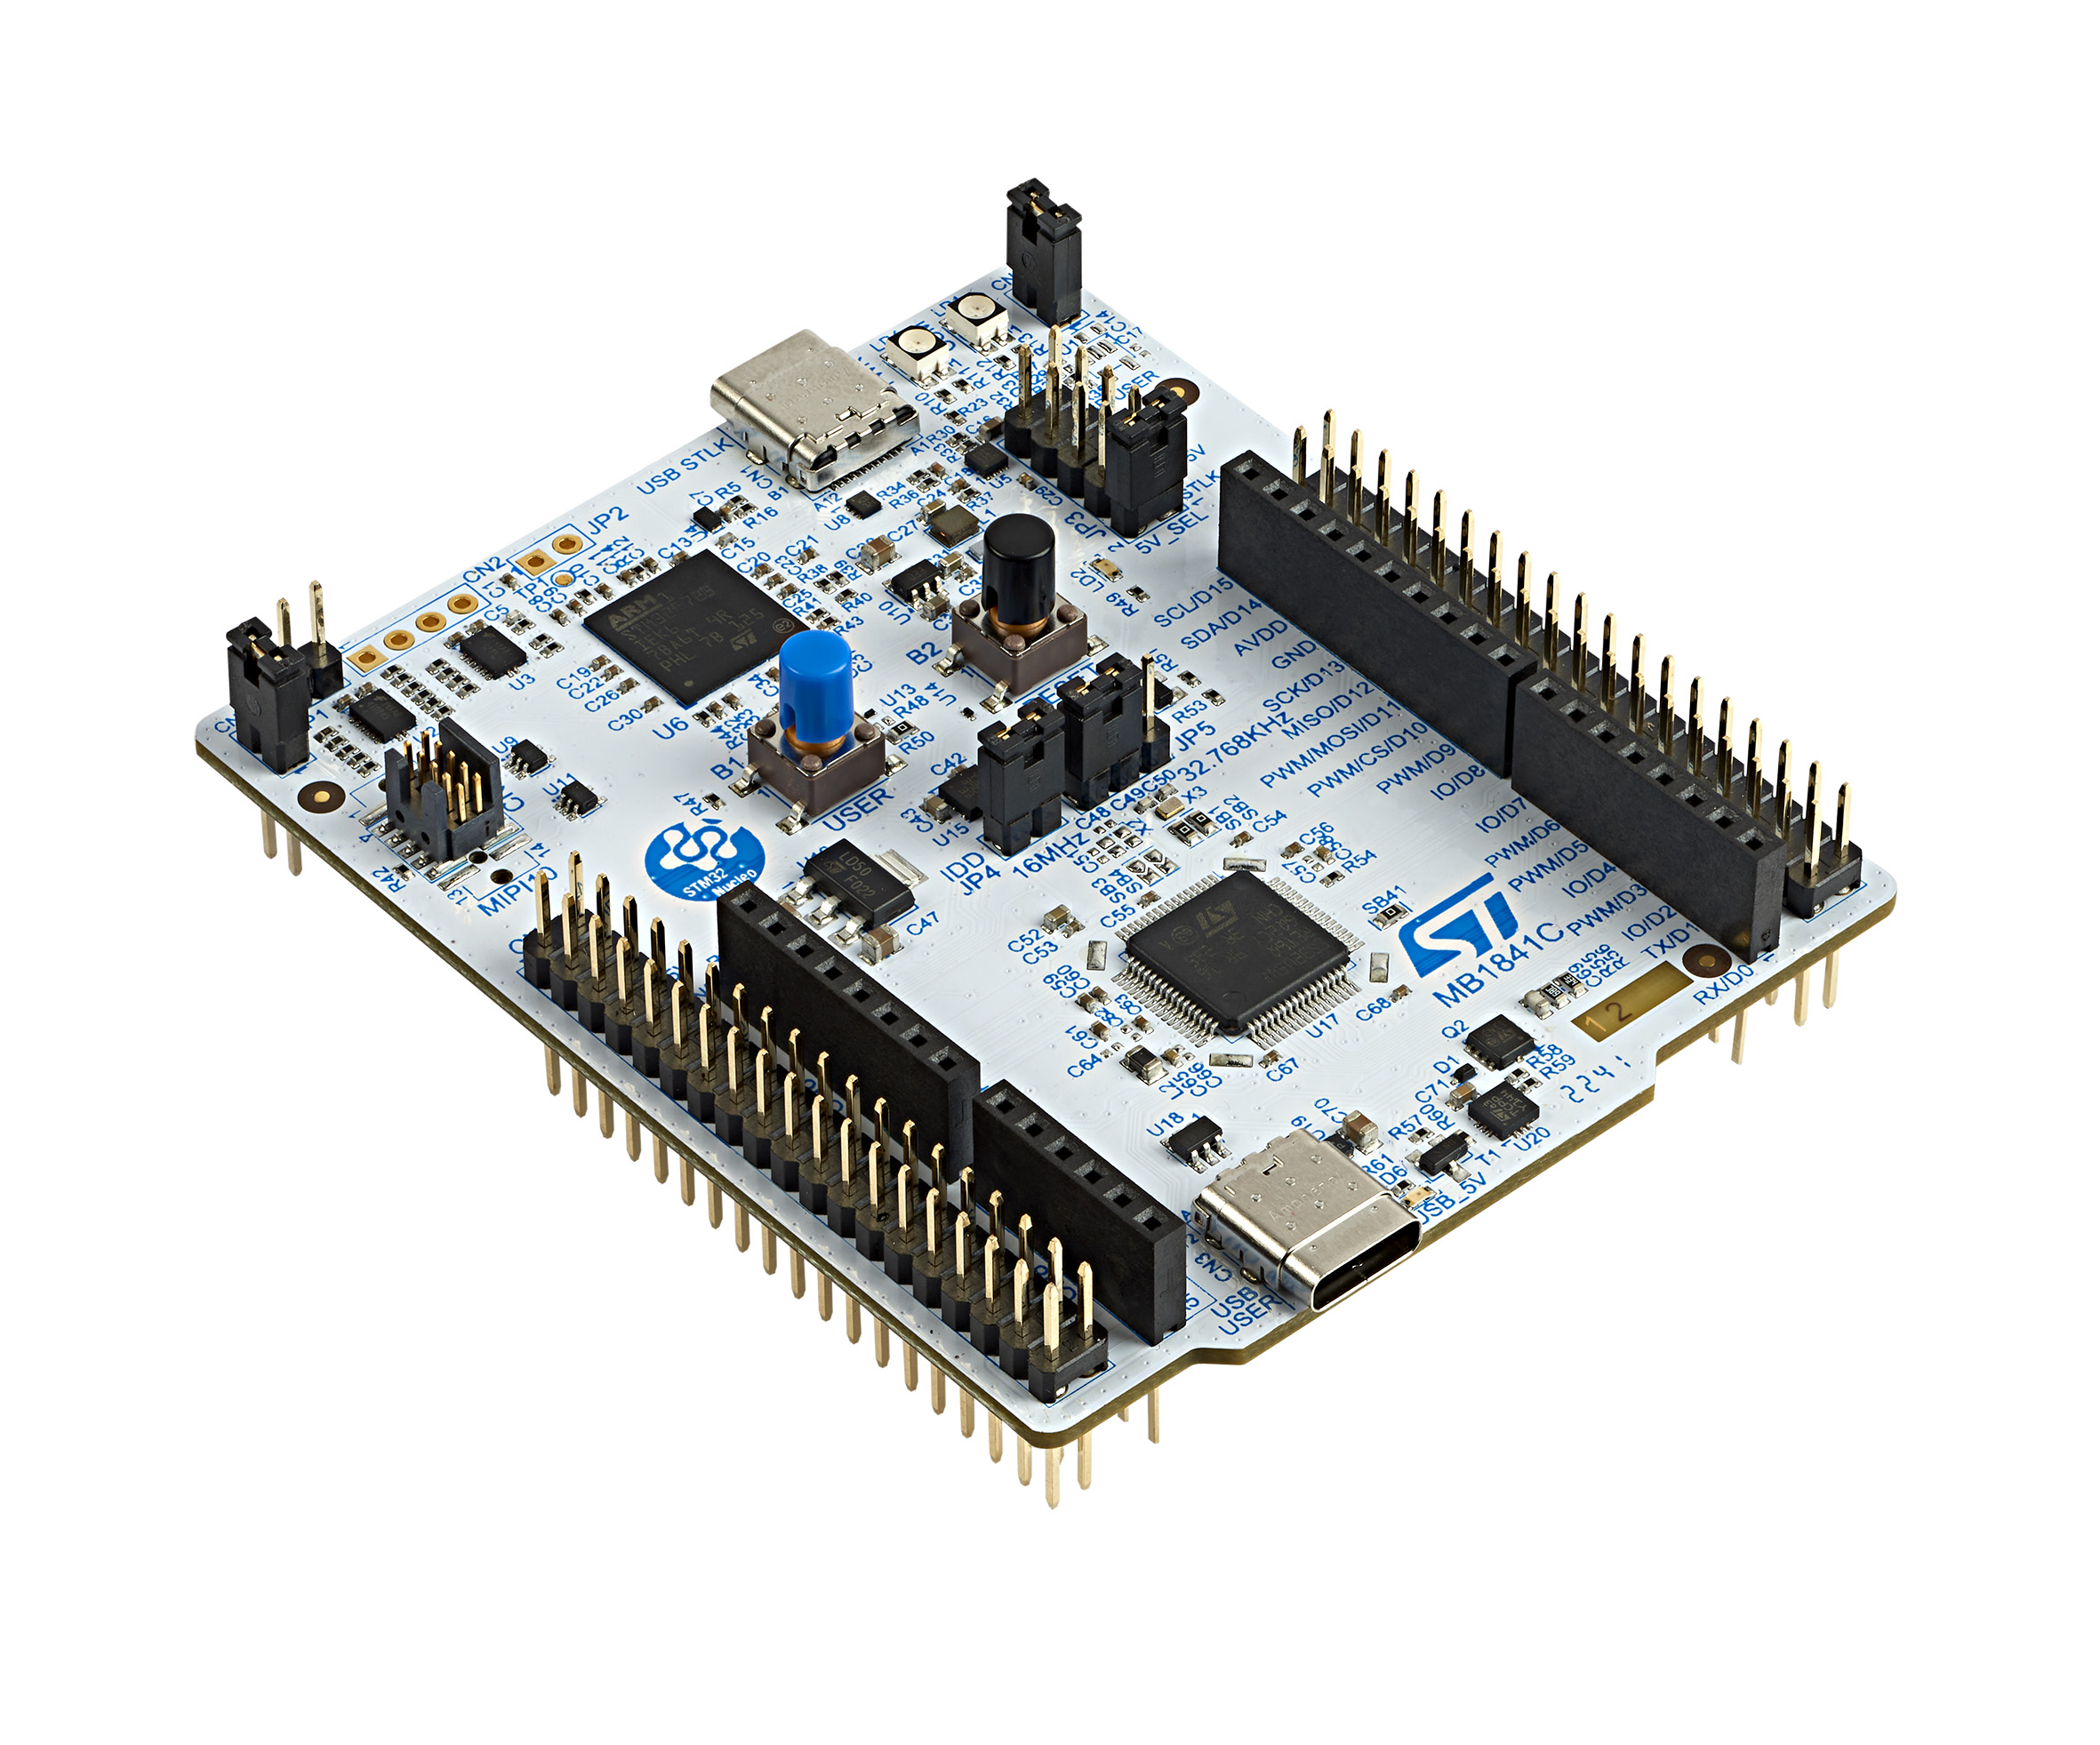
\includegraphics[width=6cm]{img/U5 Nucleo.jpg}
  \caption{STM32U545 Nucleo Board}
  \label{fig:IAR}
\end{figure}
\end{itemize}

\subsection{Software Resources}
The following software tools were used for the  development, debugging and testing of the "CryptoEngine" demonstration:

\subsubsection{IAR Embedded Workbench}
IAR Embedded Workbench is an integrated development environment (IDE) used for programming, debugging, and optimizing embedded applications. It provides comprehensive support for STM32 microcontrollers, including the STM32XX and STM32U5 series. Key features include:
\begin{itemize}
    \item Advanced debugging capabilities with breakpoints, watch windows, and real-time data visualization.
    \item Code optimization tools to improve performance and reduce memory footprint.
    \item Integrated support for STM32CubeMX, allowing seamless project setup and configuration.
\end{itemize}
\begin{figure}[H]
  \centering
  
\includegraphics[width=8cm]{img/IAR.png}
  \caption{IAR Embedded Workbench}
  \label{fig:IAR}
\end{figure}

\subsubsection{STM32CubeMX}
STM32CubeMX is a graphical software configuration tool that simplifies the development of STM32-based applications. It allows developers to:
\begin{itemize}
    \item Configure microcontroller peripherals and middleware components through an intuitive graphical interface.
    \item Generate initialization code for STM32 microcontrollers, reducing development time.
    \item Integrate with various IDEs, including IAR Embedded Workbench, for a streamlined development workflow.
\end{itemize}
\begin{figure}[H]
  \centering
  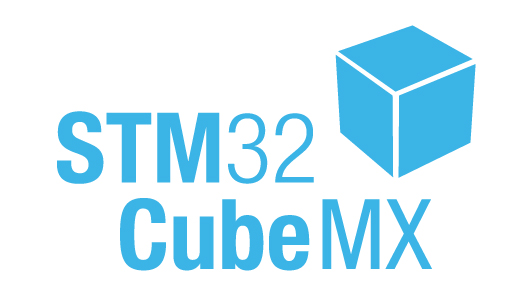
\includegraphics[width=8cm]{img/CUBEMX.jpg}
  \caption{STM32CubeMX}
  \label{fig:mx}
\end{figure}
\subsubsection{Yet Another Terminal (YAT)}
Yet Another Terminal (YAT) is a terminal application used for serial communication with the STM32 microcontrollers. It provides a user-friendly interface for monitoring and interacting with the microcontroller's output. Key features include:
\begin{itemize}
    \item Support for multiple communication protocols, including USART.
    \item Real-time data logging and visualization capabilities.
    \item Customizable settings for baud rate, data bits, parity, and stop bits.
\end{itemize}
\section*{Conclusion}
The work environment for this internship project includes both hardware and software resources that are essential for the successful implementation and demonstration of the "CryptoEngine" peripheral. The STM32XX MCU provides the necessary hardware capabilities, while the STM32U545 MCU is used for comparison and interoperability, utilizing AES and PKA peripherals. IAR Embedded Workbench and STM32CubeMX offer powerful tools for software development and configuration. Together, these resources enable the creation of a secure, efficient, and user-friendly cryptographic demonstration.

        \clearpage
        
        \chapter{Solution Implementation}
\label{ch:implementation}

\section*{Introduction}
In this chapter, we provide a detailed step-by-step explanation of the implementation of the "CryptoEngine" demo. This demo showcases the use of cryptographic techniques to establish secure communication between two microcontrollers, specifically the STM32XX and STM32U545 MCUs.

\section{Demo Overview}
The following section outlines the sequence of operations involved in the "CryptoEngine" demo.
The steps are detailed in Table \ref{tab:authenticated_encryption_steps}:
\begin{longtable}{|c|p{6cm}|p{6cm}|}
\caption{Steps for "CryptoEngine" Demo} \label{tab:authenticated_encryption_steps} \\

\hline
\textbf{Step} & \textbf{Alice} & \textbf{Bob} \\
\hline
\endfirsthead

\multicolumn{3}{c}%
{{\bfseries \tablename\ \thetable{} -- continued from previous page}} \\
\hline
\textbf{Step} & \textbf{Alice} & \textbf{Bob} \\
\hline
\endhead

\hline \multicolumn{3}{|r|}{{Continued on next page}} \\ \hline
\endfoot

\hline
\endlastfoot

1 & Generate ECDSA Key Pair & Generate ECDSA Key Pair \\
  & \multicolumn{2}{p{12cm}|}{\textit{(ECDSA keys are used for creating and verifying digital signatures)}} \\
\hline
2 & Generate ECDH Key Pair & Generate ECDH Key Pair \\
  & \multicolumn{2}{p{12cm}|}{\textit{(ECDH keys are used for establishing a shared secret)}} \\
\hline
3 & Send ECDSA Public Key + Signature to Bob & Send ECDSA Public Key + Signature to Alice \\
\hline
4 & Verify Bob's Signature using his ECDSA Public Key & Verify Alice's Signature using her ECDSA Public Key \\
  & \multicolumn{2}{p{12cm}|}{\textit{(Ensures the authenticity of the participants)}} \\
\hline
5 & Send ECDH Public Key to Bob & Send ECDH Public Key to Alice \\
\hline
6 & Compute ECDH Shared Secret using own Private ECDH Key and Bob's Public ECDH Key & Compute ECDH Shared Secret using own Private ECDH Key and Alice's Public ECDH Key \\
  & \multicolumn{2}{p{12cm}|}{\textit{(Shared secret is used as the basis for deriving encryption keys)}} \\
\hline
7 & Derive AES GCM Key and IV from ECDH Shared Secret & Derive AES GCM Key and IV from ECDH Shared Secret \\
 
\hline
8 & Encrypt and Send Message using AES GCM & Decrypt and Verify Message using AES GCM \\
\hline
9 & Decrypt and Verify Response using AES GCM & Encrypt and Send Response using AES GCM \\
\hline

\end{longtable}

\section{Sequence Diagram}
\begin{figure}[H]
  \centering
  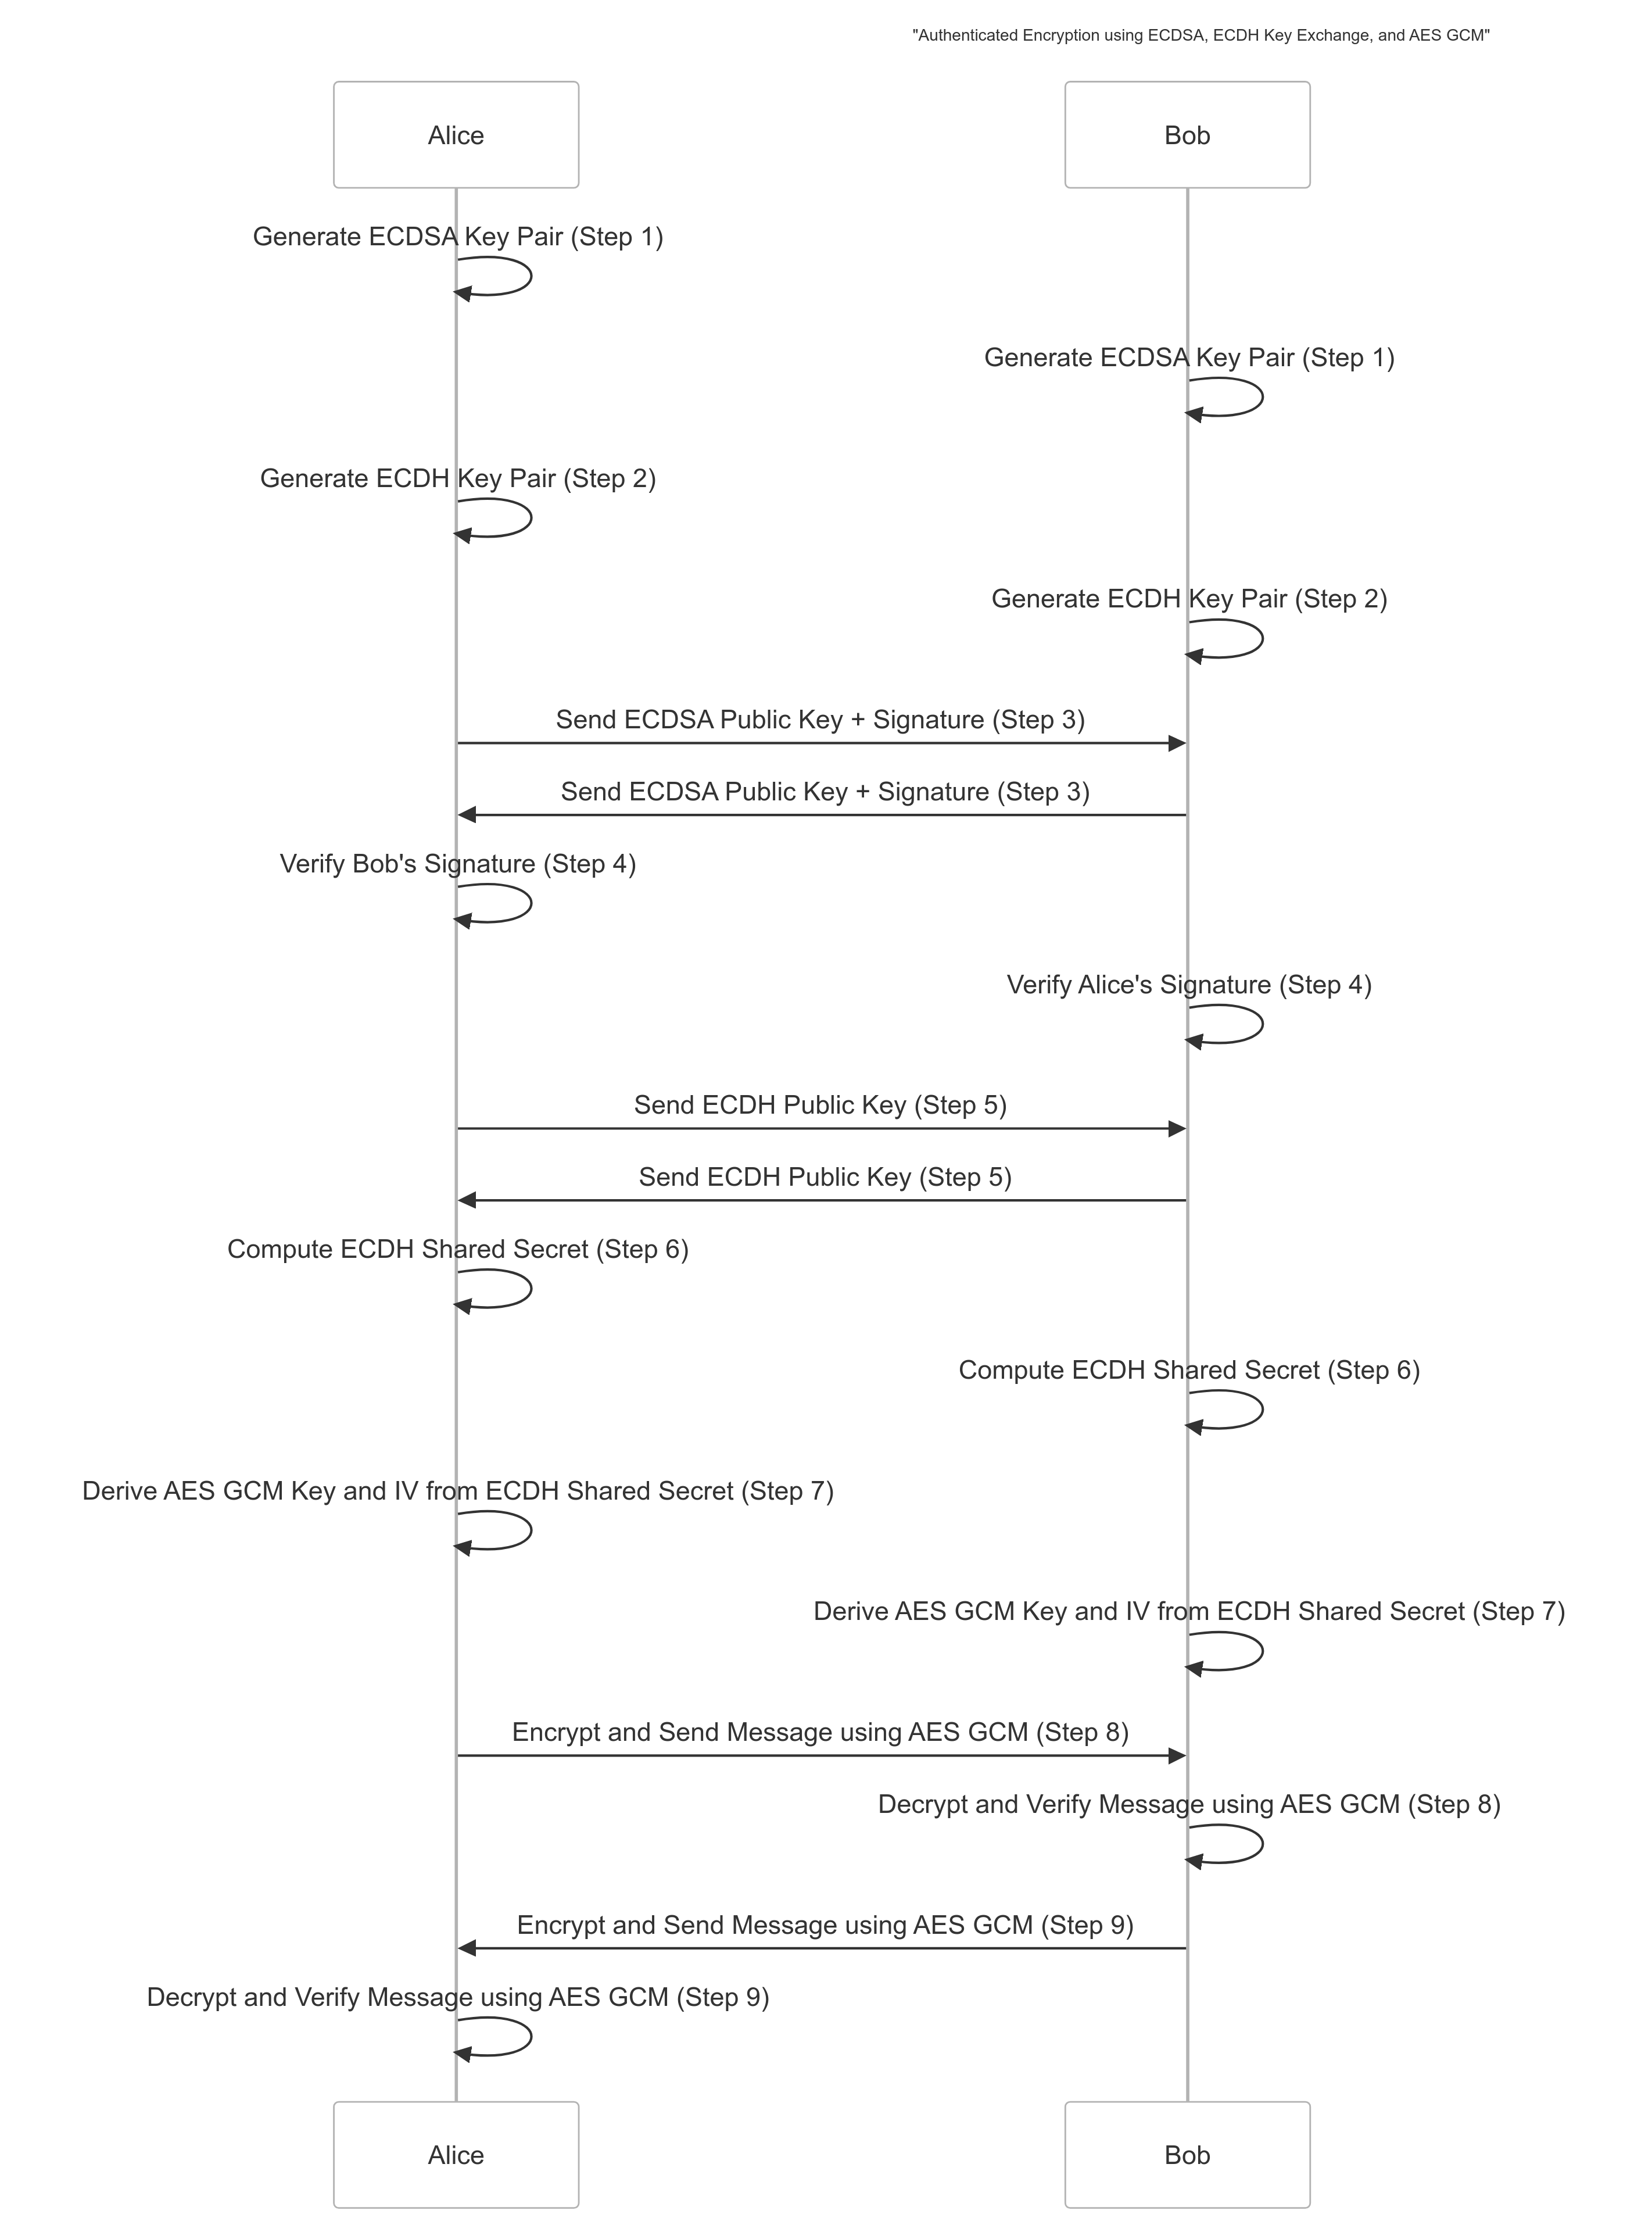
\includegraphics[width=17cm]{img/numbered auth enc.png}
  \caption{Sequence Diagram for "CryptoEngine" Demo }
  \label{fig:sequence_diagram}
\end{figure}

\hspace{1cm}The Sequence Diagram in Figure \ref{fig:sequence_diagram} illustrates the process of authenticated encryption using ECDSA for authentication, ECDH for key exchange, and AES GCM for encryption. The diagram shows the interactions between two participants, Alice and Bob, as they perform cryptographic operations to securely exchange messages.

\textit{Note : In our demo, the STM32XX and STM32U545 MCUs will play the roles of Alice and Bob respectively.}



This sequence diagram demonstrates a secure communication process where both participants authenticate each other using ECDSA, establish a shared secret using ECDH, and securely exchange messages using AES GCM. The use of these cryptographic techniques ensures the confidentiality, integrity, and authenticity of the exchanged messages.

\section{Demonstration Details and Explanation}
For confidentiality reasons we will only detail the "Bob" side of the demo, since it is using the STM32U545 MCU.

\subsection{ECDSA Key Pair Generation}
This is the first step of the demo. It involves setting up PKA peripheral to generate the public ECDSA key.
    \subsubsection{PKA Peripheral Initialization}
        To compute ECDSA public key we need to set the PKA mode to "ECC Fp scalar multiplication", then we need to input the cryptographic parameters in the correct addresses in PKA RAM.
    \subsubsection{ECC Scalar Multiplication }
        To input cryptographic parameters in PKA RAM, we need to refer to the STM32U5 reference manual \cite{U5_Refman} where we can find the specifications for using ECC Fp scalar multiplication.
        The details of this operation can be found in Figure \ref{fig:PKA ECC}.

         This figure details the address and size of every cryptography parameter involved in ECC multiplication, which we are using at this level to compute the ECDSA public key.
 Note that in our demonstration, since we are using a 256-bit curve, the size labeled as EOS (ECC Operand Size) is equal to 320 bits which are 256 bits of actual data and 64 bits of zeros which are necessary when inputting certain data to PKA RAM, as mentioned in the reference manual for U5 \cite{U5_Refman}.

\begin{figure}[H]
    \centering
    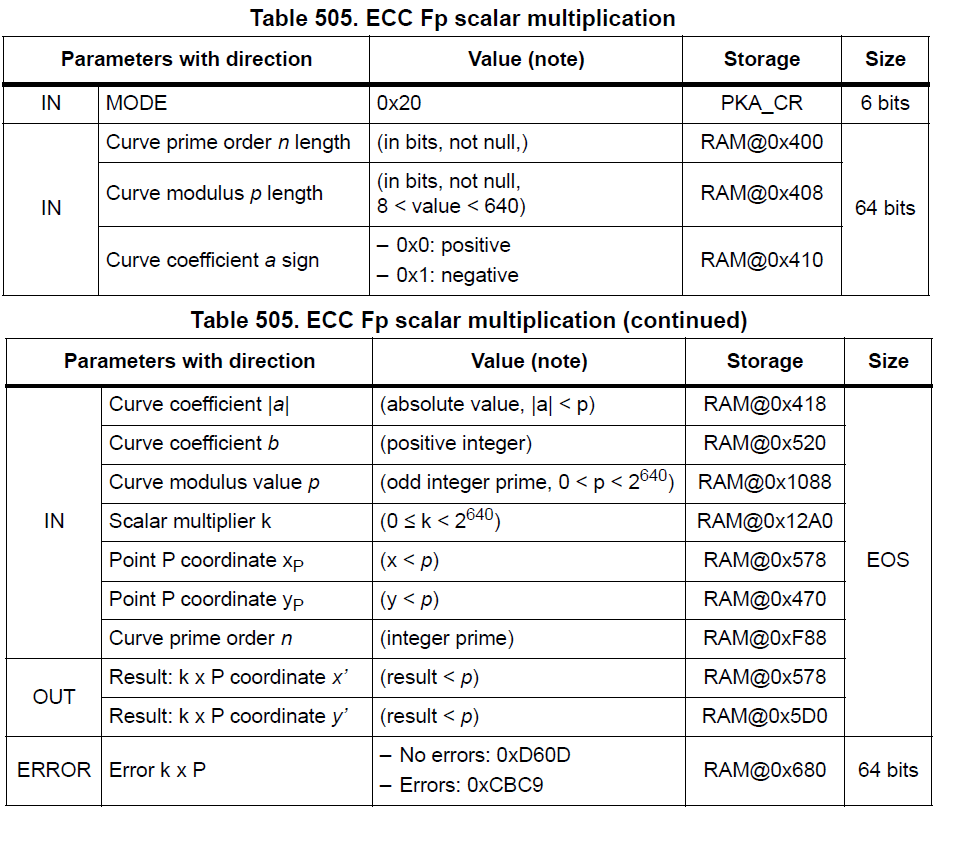
\includegraphics[width=15cm]{img/PKA ECC.png}
    \caption{PKA ECC Fp Scalar Multiplication}
    \label{fig:PKA ECC}
\end{figure}




 In our case the parameters that we need to use are provided by NIST \cite{Nist_curve} and are specified in the following table.

 
\begin{longtable}{|c|p{13cm}|}

\caption{NIST P-256 Curve Specifications} \\
\hline
\textbf{Name} & \textbf{Value} \\
\hline
\endfirsthead

\multicolumn{2}{c}%
{{\bfseries NIST P-256 Curve Specifications (continued)}} \\
\hline
\textbf{Name} & \textbf{Value} \\
\hline
\endhead

\hline \multicolumn{2}{|r|}{{Continued on next page}} \\ \hline
\endfoot

\hline \hline
\endlastfoot

Curve Modulus p & 0xffffffff00000001000000000000000000000000ffffffffffffffffffffffff \\
\hline
Curve Coefficient a & 0xffffffff00000001000000000000000000000000fffffffffffffffffffffffc \\
\hline
Curve Coefficient b & 0x5ac635d8aa3a93e7b3ebbd55769886bc651d06b0cc53b0f63bce3c3e27d2604b \\
\hline
Generator Point G & \begin{tabular}{@{}p{12cm}@{}} (0x6b17d1f2e12c4247f8bce6e563a440f277037d812deb33a0f4a13945d898c296, \\ 0x4fe342e2fe1a7f9b8ee7eb4a7c0f9e162bce33576b315ececbb6406837bf51f5) \end{tabular} \\
\hline
Curve prime order n & 0xffffffff00000000ffffffffffffffffbce6faada7179e84f3b9cac2fc632551 \\
\end{longtable}
\textit{Note : These same curve parameters will be reused for ECDSA signature generation and verification as well as ECDH key pair generation.
}

These curve specifications have to be put in their specific adresses in PKA RAM in order to set the stage for elliptic curve operations on the P-256 curve. 

Figure \ref{fig:curvo} demonstrates the code implementation of the curve parameters.


\begin{figure}[H]
    \centering
    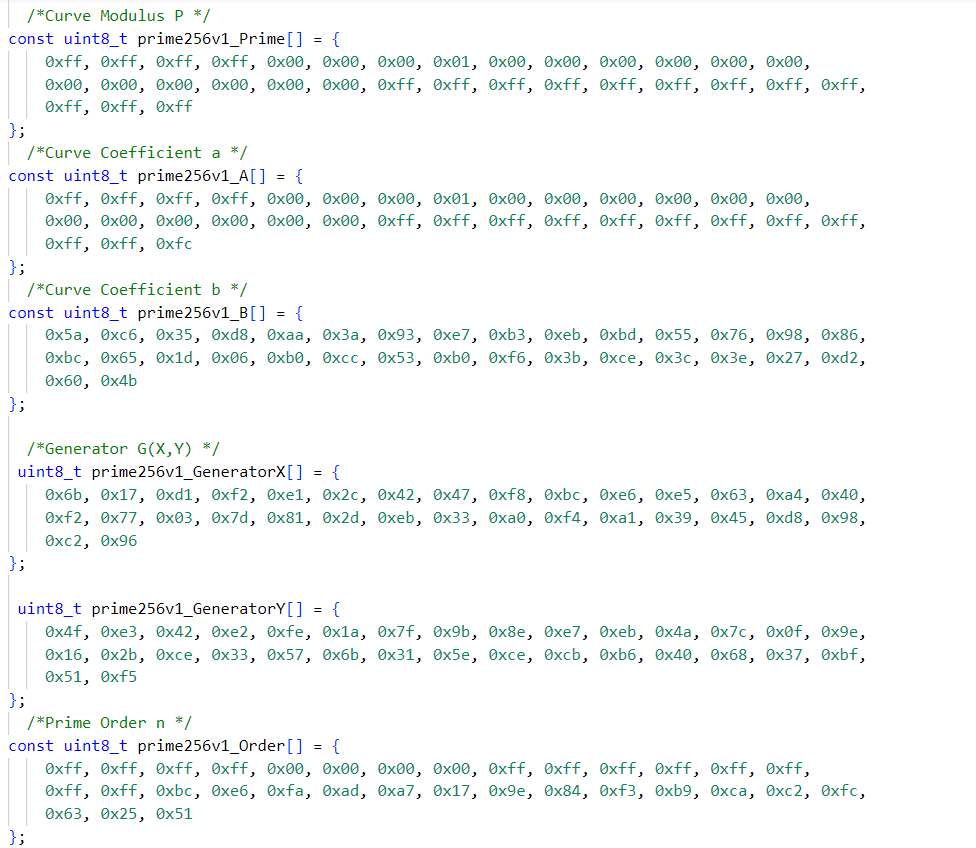
\includegraphics[width=19cm]{img/ecdsa curve params code.png}
    \caption{Code Implementation of NIST P-256 Parameters}
    \label{fig:curvo}
\end{figure}

We will use PKA structures provided by the Hardware Abstraction Layer (HAL) to configure our curve parameters, as illustrated in Figure \ref{fig:ecc struct}.
We have developed a function to fill in this structure's members with the NIST P-256 curve parameters as illustrated in Figure \ref{fig:pka_ecc_func}

\begin{figure}[H]
    \centering
    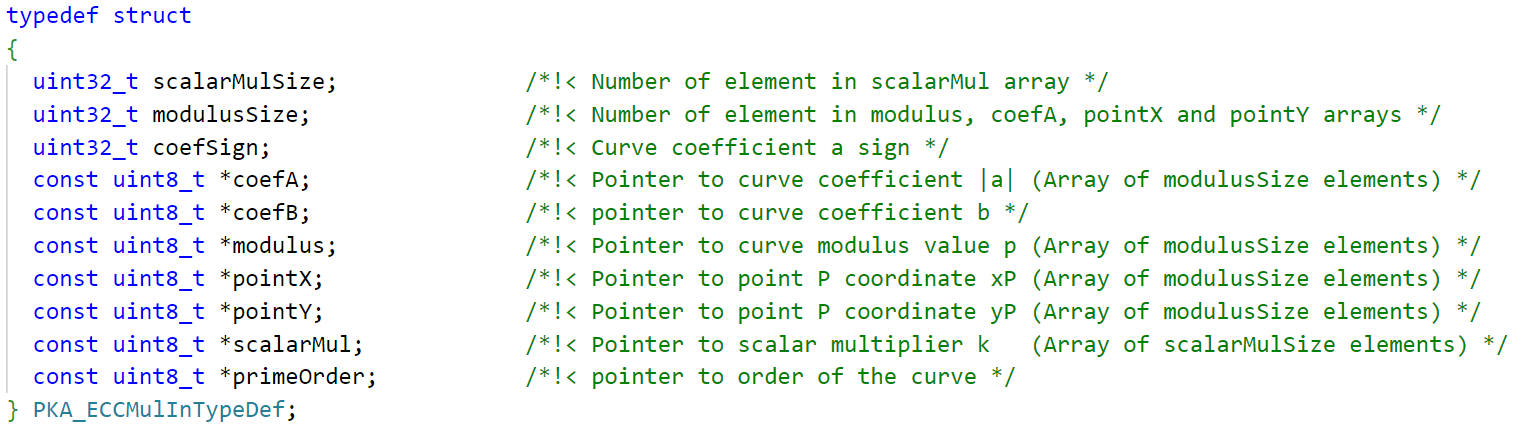
\includegraphics[width=18cm]{img/ecc struct.png}
    \caption{HAL PKA ECC Input Structure}
    \label{fig:ecc struct}
\end{figure}


\begin{figure}[H]
    \centering
    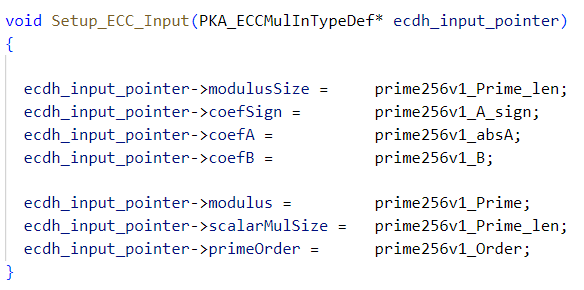
\includegraphics[width=15cm]{img/ecc func.png}
    \caption{PKA ECC Setup}
    \label{fig:pka_ecc_func}
\end{figure}

After setting up the elliptic curve parameters, we can generate the ECDSA public key using the ECDSA private key illustrated in Figure \ref{fig:ecdsa_priv_key}. Figure \ref{fig:pka_ecdsa_generate} shows the function used to generate the public key, and Figure \ref{fig:pka_pubkey_terminal1} shows the generated key, transmitted through USART to our terminal application. As previously mentioned in \ref{curve_param}, the ECDSA public key is a point on the elliptic curve which has a X and Y coordinate, each of them being 256 bits.

\begin{figure}[H]
    \centering
    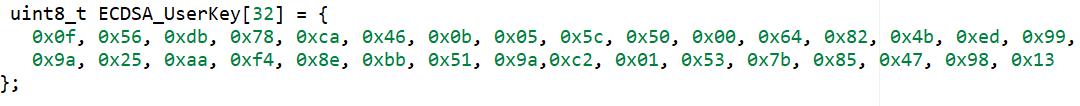
\includegraphics[width=18cm]{img/ecdsa priv key.png}
    \caption{ECDSA Private Key}
    \label{fig:ecdsa_priv_key}
\end{figure}


\begin{figure}[H]
    \centering
    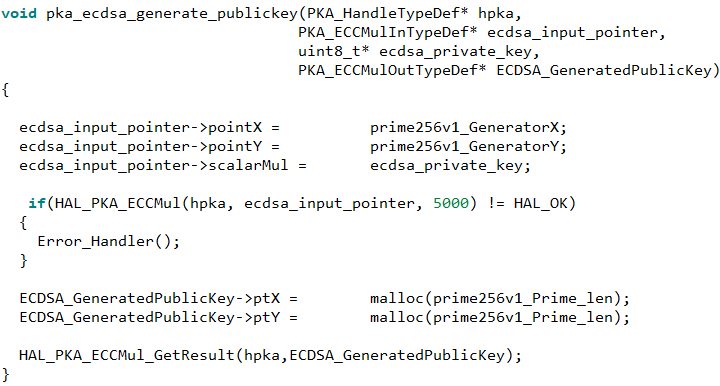
\includegraphics[width=16cm]{img/pka_generate_ecdsa.png}
    \caption{ECDSA Public Key Generation Function}
    \label{fig:pka_ecdsa_generate}
\end{figure}





\begin{figure}[H]
    \centering
    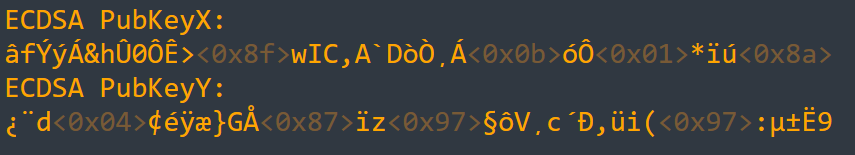
\includegraphics[width=15cm]{img/ecdsa pubkey.png}
    \caption{Generated ECDSA Public Key}
    \label{fig:pka_pubkey_terminal1}
\end{figure}

\subsection{ECDH Key Pair Generation}
This is the second step of the demo. Similarly to the previous step, we will use PKA to generate the ECDH public key.

    \subsubsection{ECC Scalar Multiplication}
    The key generation process using "ECC Fp scalar multiplication" is the same for ECDSA and ECDH, as described in Figure \ref{fig:PKA ECC}. We will use the same PKA structure as in ECDSA key generation as illustrated in Figure \ref{fig:ecc struct}.

    The ECDH private key illustrated in Figure \ref{fig:ecdh_priv} is used along with the function shown in Figure \ref{fig:ecc_generate} in order to generate the ECDH public key, which is shown in Figure \ref{fig:ecc_pub}.
    \begin{figure}[H]
    \centering
    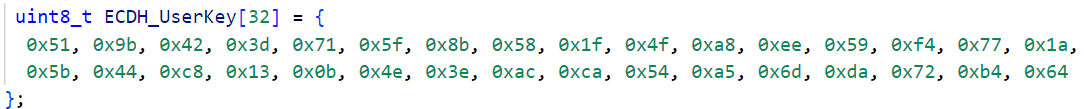
\includegraphics[width=15cm]{img/ecdh private}
    \caption{ECDH Private Key}
    \label{fig:ecdh_priv}
    \end{figure}

    \begin{figure}[H]
    \centering
    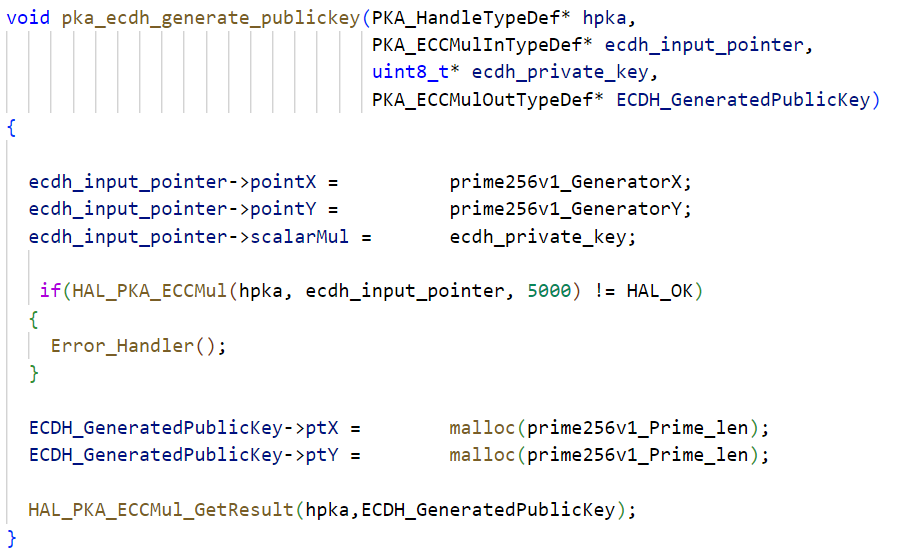
\includegraphics[width=13cm]{img/ecdh generate.png}
    \caption{ECDH Public Key Generation Function}
    \label{fig:ecc_generate}
    \end{figure}

    \begin{figure}[H]
    \centering
    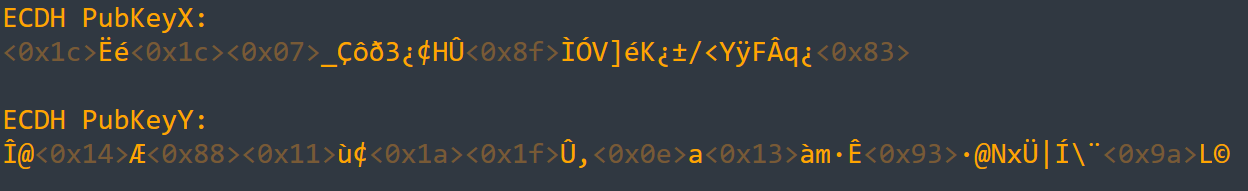
\includegraphics[width=13cm]{img/ecdh pub key.png}
    \caption{Generated ECDH Public Key }
    \label{fig:ecc_pub}
    \end{figure}

\subsection{ECDSA Signature Generation}    
%In order to ensure authenticity of the message exchange, we need to generate an ECDSA signature that will be sent along with the ECDSA public key to be used for signature verification.

To generate an ECDSA signature, we will use the PKA mode illustrated in Figure \ref{fig:ecdsa_sign_tab} \cite{U5_Refman}.
 \begin{figure}[H]
    \centering
    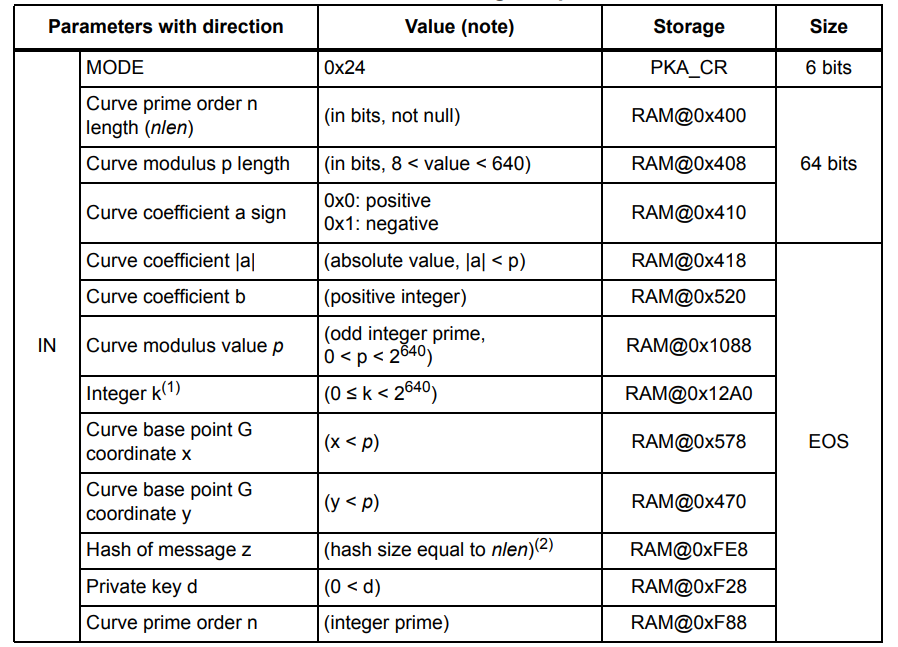
\includegraphics[width=14cm]{img/ecdsa sign2.png}
    \caption{ECDSA Sign Operation }
    \label{fig:ecdsa_sign_tab}
    \end{figure}

 We will use the PKA ECDSA signature structure provided by the HAL driver shown in Figure \ref{fig:ecdsa struct} along with the function shown in \ref{fig:ecdsa func} to input the signature parameters in PKA RAM.

\begin{figure}[H]
    \centering
    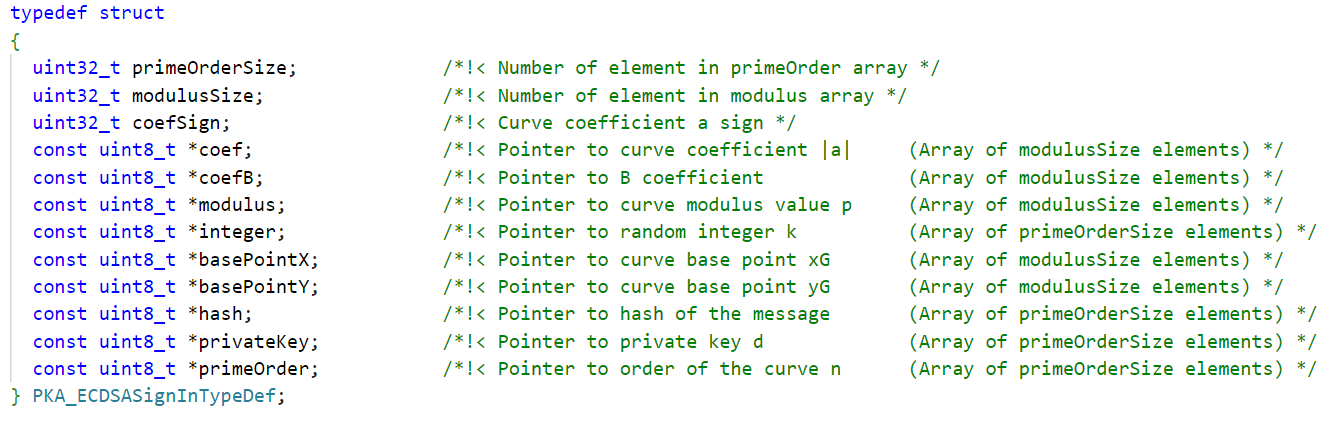
\includegraphics[width=17cm]{img/ecdsa struct.png}
    \caption{HAL PKA ECDSA Input Structure}
    \label{fig:ecdsa struct}
    \end{figure}

    \begin{figure}[H]
    \centering
    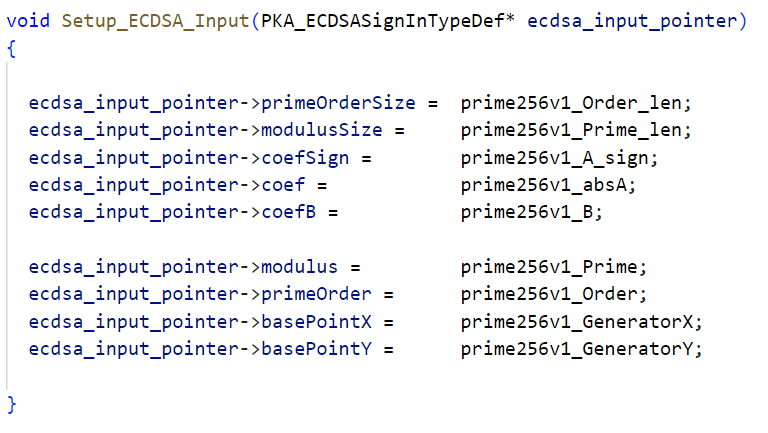
\includegraphics[width=17cm]{img/ecdsa_func.png}
    \caption{HAL PKA ECDSA Input Structure}
    \label{fig:ecdsa func}
    \end{figure}

    Compared to public key generation, generating the signature requires a new private parameter called "k" which is a 256-bit number only used once to generate the signature. The integer "k" used for this demo is shown in Figure \ref{fig:ecdsa_k}. The signature generation also uses a hash message, which in our demonstration is pre-shared between the two parties.
    \begin{figure}[H]
    \centering
    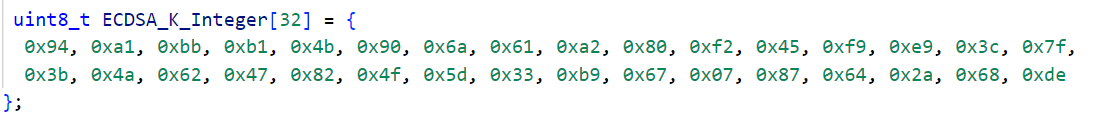
\includegraphics[width=17cm]{img/ecdsa k.png}
    \caption{ECDSA Integer "K"}
    \label{fig:ecdsa_k}
    \end{figure}
    After setting up the ECDSA HAL structure, we can launch the ECDSA signing operation using the function shown in Figure \ref{fig:ecdsa func2}.
    \begin{figure}[H]
    \centering
    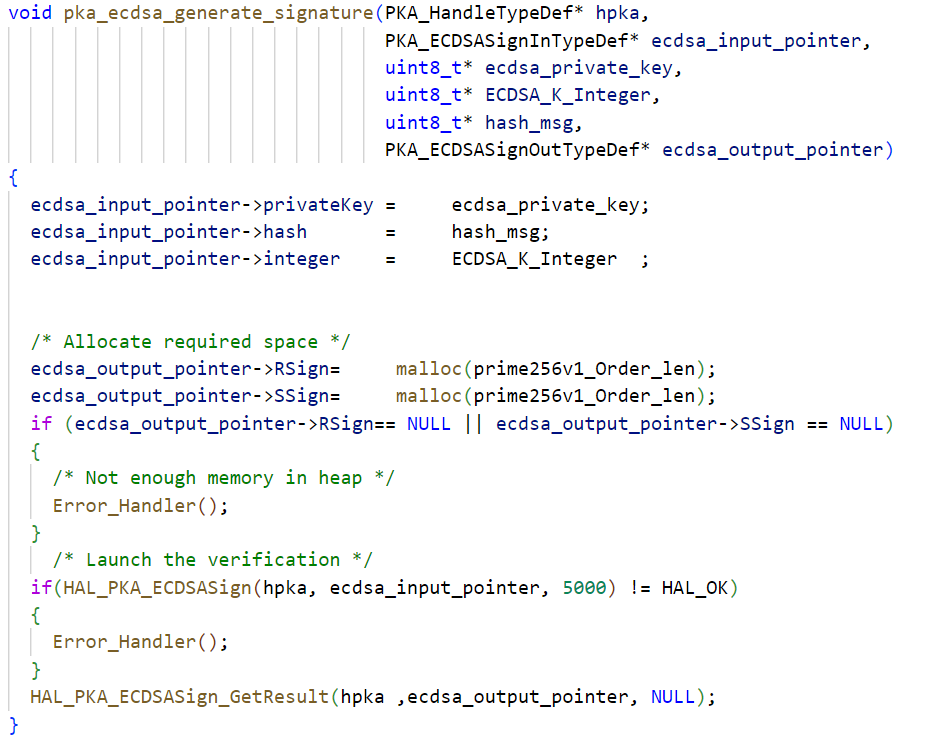
\includegraphics[width=17cm]{img/ecdsa func2.png}
    \caption{ECDSA Signing Function}
    \label{fig:ecdsa func2}
    \end{figure}

    The generated signature is composed of two parts "Signature R" and "Signature S", each being 256 bits long. Figure \ref{fig:ecdsa_rs} shows the output of the signing operation.
    
    \begin{figure}[H]
    \centering
    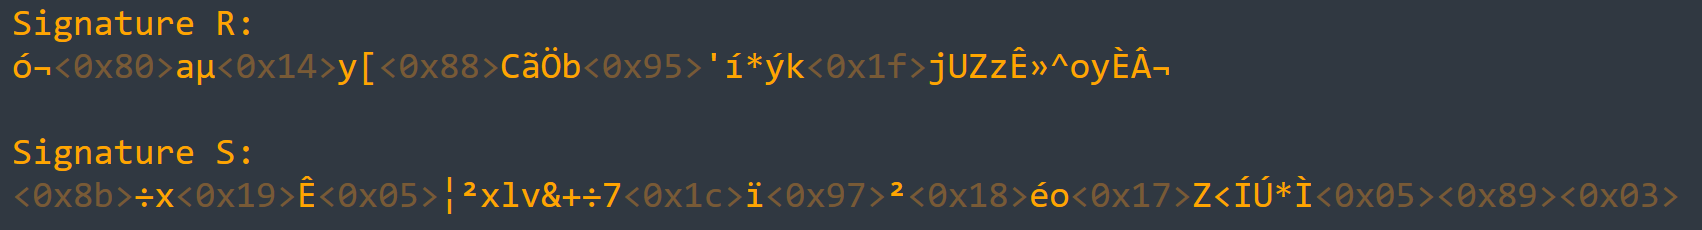
\includegraphics[width=17cm]{img/signature rs.png}
    \caption{Generated ECDSA Signature}
    \label{fig:ecdsa_rs}
    \end{figure}

    \subsection{ECDSA Public Key and Signature Exchange}
    After having generated the ECDSA public keys and signatures, the two MCUs exchange these parameters using USART. Exchanging these parameters is crucial for the following step, which is signature verification, to ensure the authenticity of the communication.
    
    Figure \ref{fig:received sign} shows the ECDSA public key and signature received by "Bob" which were generated by "Alice". 
    \begin{figure}[H]
    \centering
    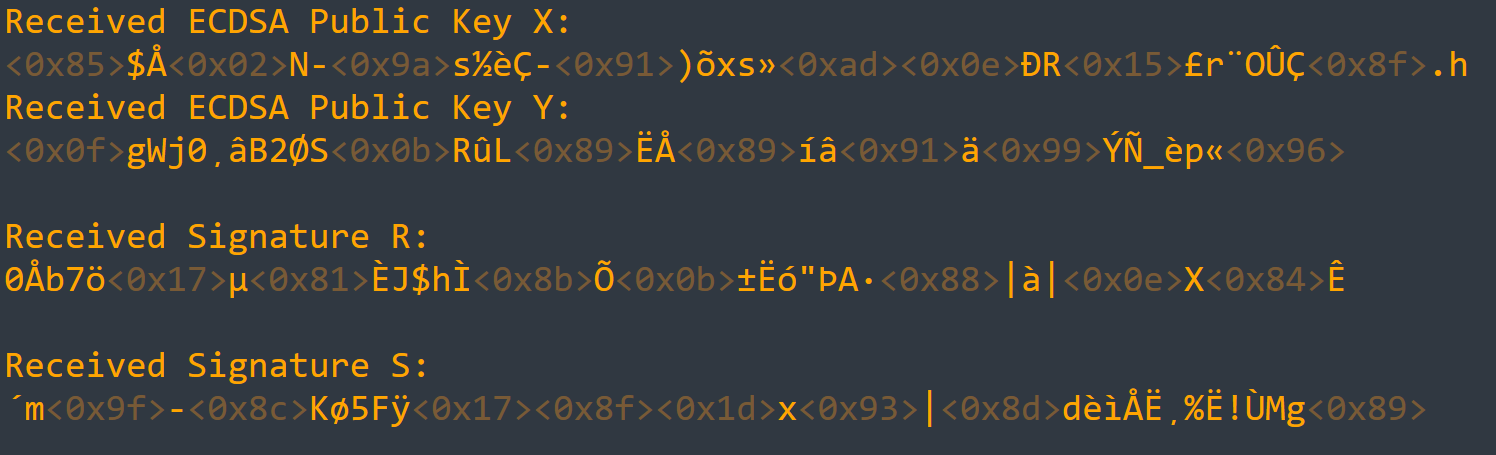
\includegraphics[width=16cm]{img/received sigpub.png}
    \caption{Received ECDSA Signature}
    \label{fig:received sign}
    \end{figure}

    \subsection{ECDSA Signature Verification}
    In this step, each device verifies the ECDSA signature sent by the other party using the PKA mode "ECDSA Verification" shown in Figure \ref{fig:ecdsa verif} \cite{U5_Refman}.
    A lot of the same curve parameters are the same as ECDSA signature generation , with the addition of the received public key and signature parameters.
    \begin{figure}[H]
    \centering
    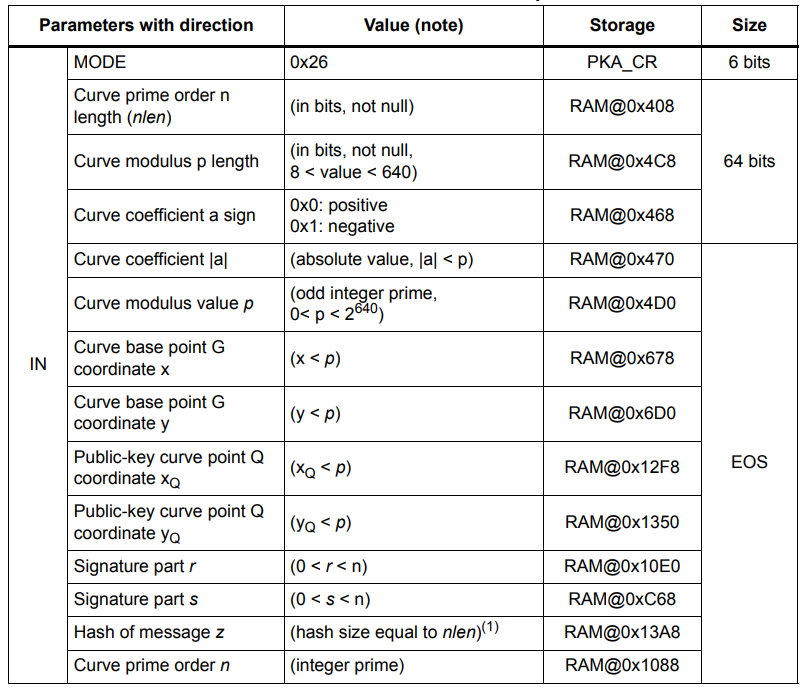
\includegraphics[width=16cm]{img/ecdsa verify.png}
    \caption{PKA "ECDSA Verification" Mode}
    \label{fig:ecdsa verif}
    \end{figure}

    Figure \ref{fig:ecdsa verif func} shows the code implementation of the ECDSA signature verification process.
    \begin{figure}[H]
    \centering
    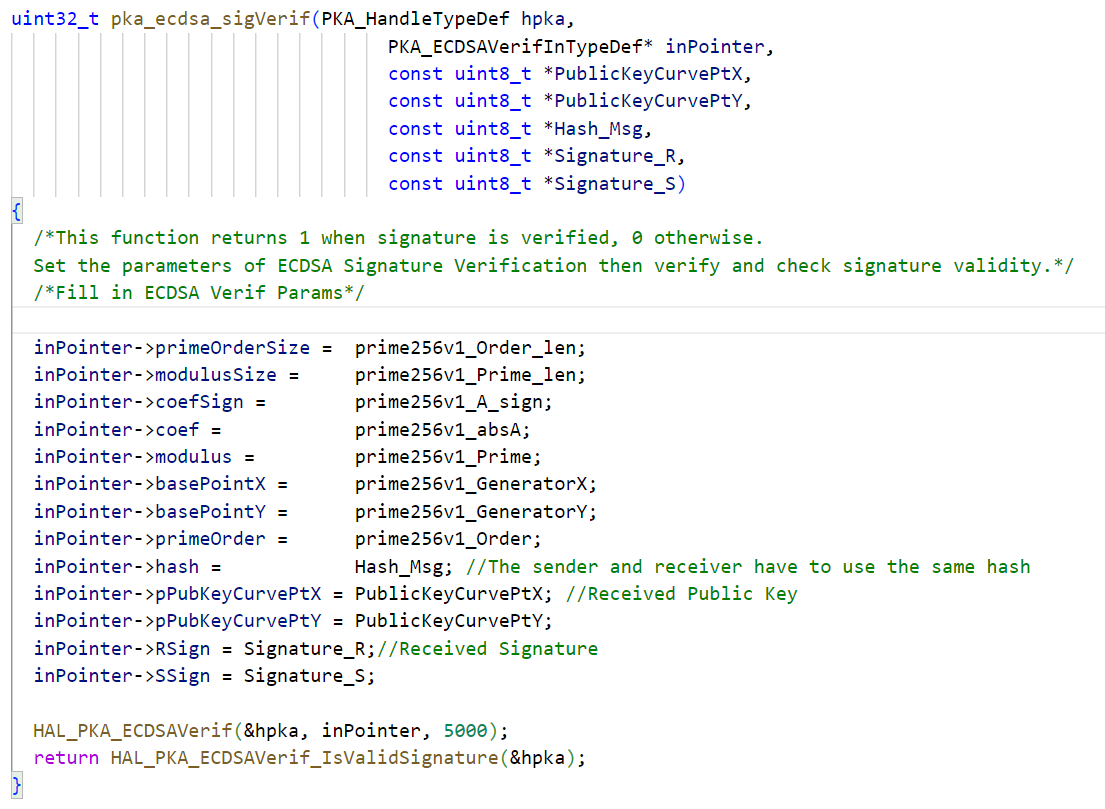
\includegraphics[width=18cm]{img/ecdsa verif func.png}
    \caption{ECDSA Verification Function }
    \label{fig:ecdsa verif func}
    \end{figure}
    
   There are two outcomes to signature verification. Figure \ref{fig:verif out} shows the output of a successful signature verification process, which allows to go on to establish ECDH key exchange, while Figure \ref{fig:ecdsa verif fail} shows the output of a failed signature verification which abruptly ends the communication. 
   
   \begin{figure}[H]
    \centering
    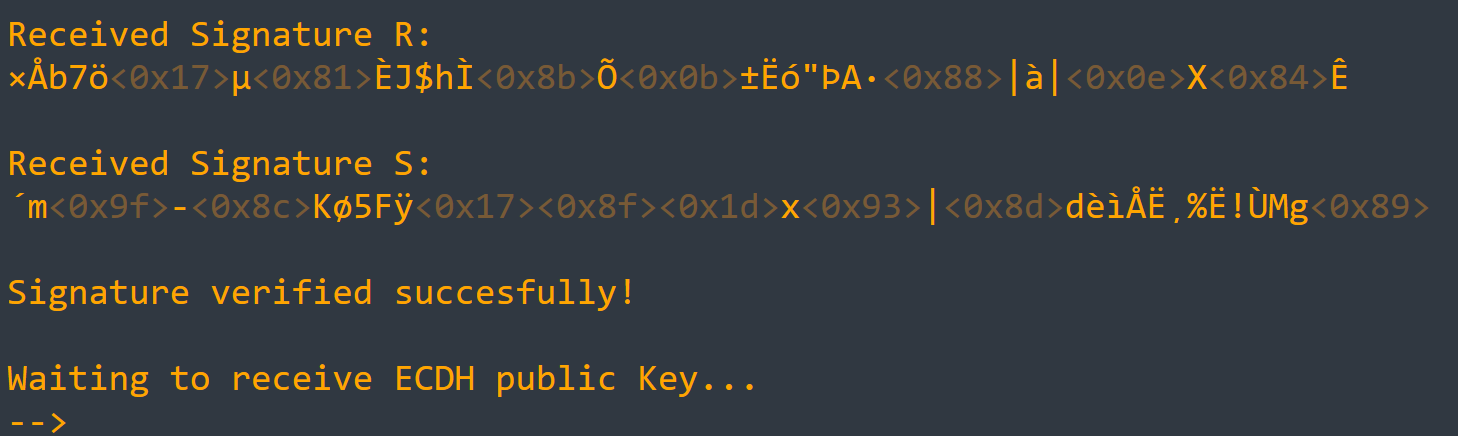
\includegraphics[width=18cm]{img/verif out.png}
    \caption{Successful ECDSA Signature Verification}
    \label{fig:verif out}
    \end{figure}
    
    \begin{figure}[H]
    \centering
    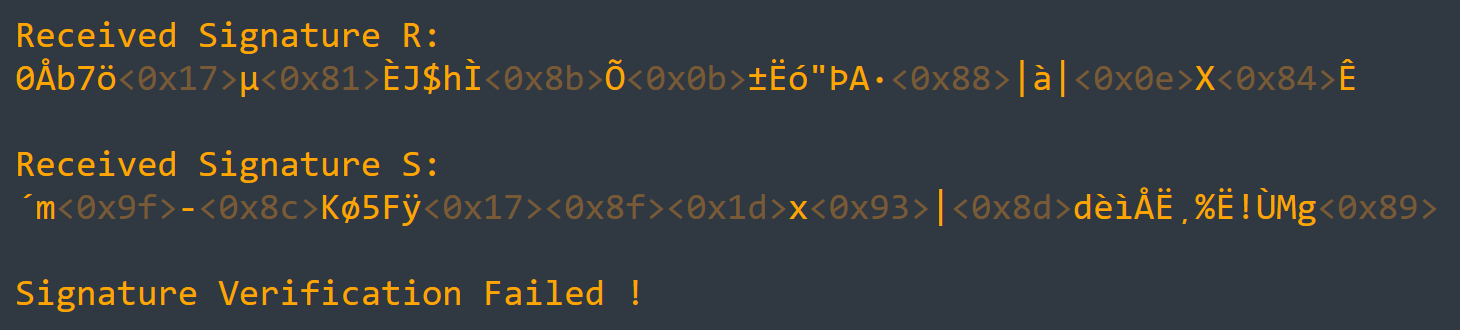
\includegraphics[width=18cm]{img/verif fail.png}
    \caption{Failed ECDSA Signature Verification}
    \label{fig:ecdsa verif fail}
    \end{figure}

    \subsection{ECDH Public Key Exchange}
    Now that the two parties have verified each other's signature, we can proceed knowing that authenticity has been assured. The next step is to establish a shared secret which will serve as a basis for establishing a symmetric encryption key. For that, the two devices must exchange the ECDH public keys generated at the start of the demo via USART. Figure \ref{fig:ecdh_pub} shows the terminal output of the ECDH public key reception process.
    
    \begin{figure}[H]
    \centering
    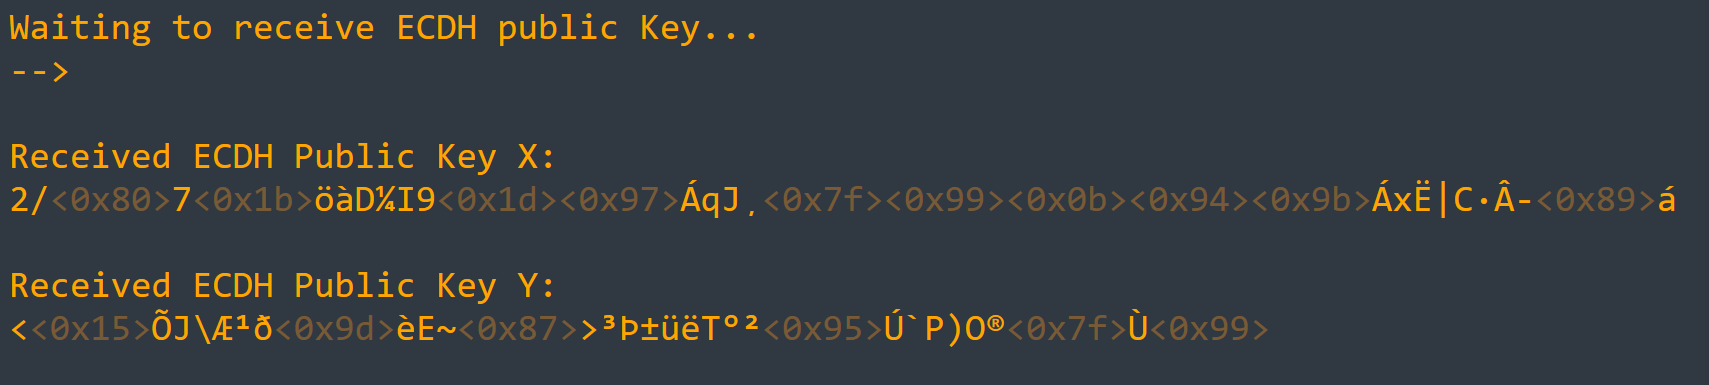
\includegraphics[width=17cm]{img/received ecdh pub.png}
    \caption{Received ECDH Public Key}
    \label{fig:ecdh_pub}
    \end{figure}
    
    \subsection{ECDH Shared Secret Generation}
    Having exchanged the ECDH public keys, each device will independently calculate the ECDH shared secret which will be a point on the elliptic curve. This point is obtained through multiplying the device's own ECDH private key with the received ECDH public key. Naturally, both devices should obtain the same common 512-bit shared secret.

    Shared secret generation is done through ECC scalar multiplication, meaning we will use the PKA mode "ECC Fp scalar multiplication" which has been detailed in Figure \ref{fig:PKA ECC} \cite{U5_Refman}.

    Figure \ref{fig:shared sec} illustrates the code implementation of ECDH shared secret generation, and Figure \ref{fig:shared sec out} shows the output result of this operation.
    \begin{figure}[H]
    \centering
    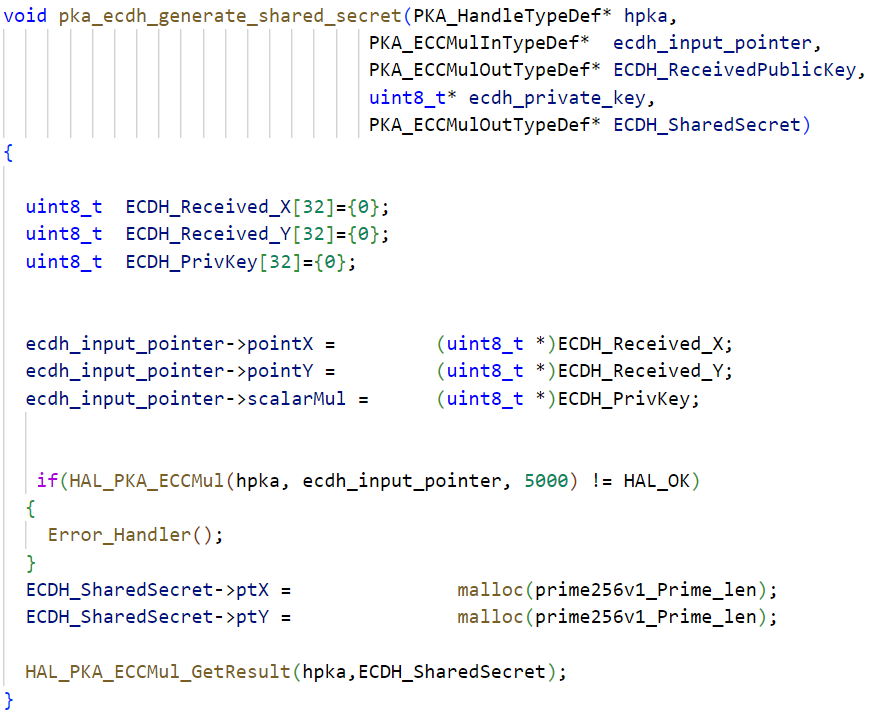
\includegraphics[width=17cm]{img/shared sec.png}
    \caption{ECDH Shared Secret Generation Function}
    \label{fig:shared sec}
    \end{figure}

    
    \begin{figure}[H]
    \centering
    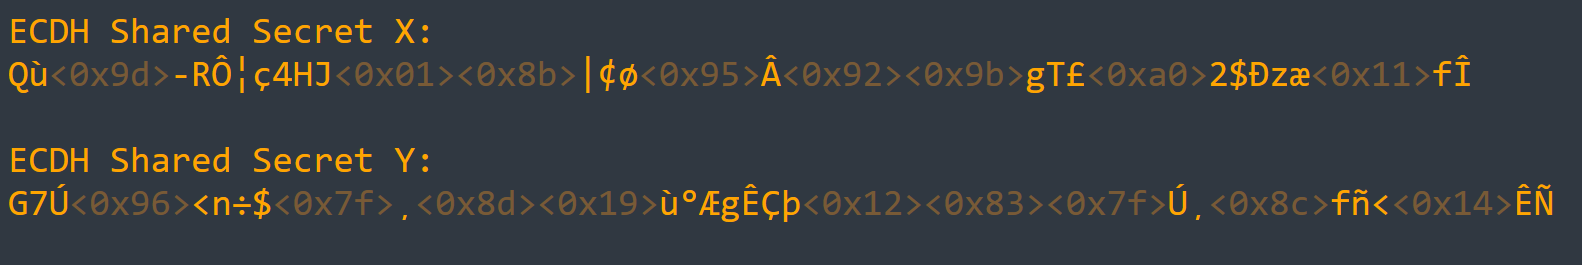
\includegraphics[width=17cm]{img/shared sec out.png}
        \caption{ECDH Shared Secret}
    \label{fig:shared sec out}
    \end{figure}
    \subsection{AES GCM Key and IV Derivation}
    Having established the shared secret, we will now derive from it the symmetric encryption key as well as the initialization vector which are needed for AES GCM .
    Usually, this process would involve a key derivation function and the use of complicated algorithms, but for the purposes of the simplicity of the demo  we opted to take the X coordinate of the ECDH shared secret as the 256-bit AES Key and the first 96 bits of the Y coordinate as the initialization vector.
    \subsection{AES GCM Symmetric Encryption}
    For this step, we will use the AES peripheral structure provided by the HAL driver provided in Figure \ref{fig:aes struct}. We will initialize the peripheral's structure as shown in Figure \ref{fig:aes init}, where we select a 256-bit key size and AES GCM mode.
    \begin{figure}[H]
    \centering
    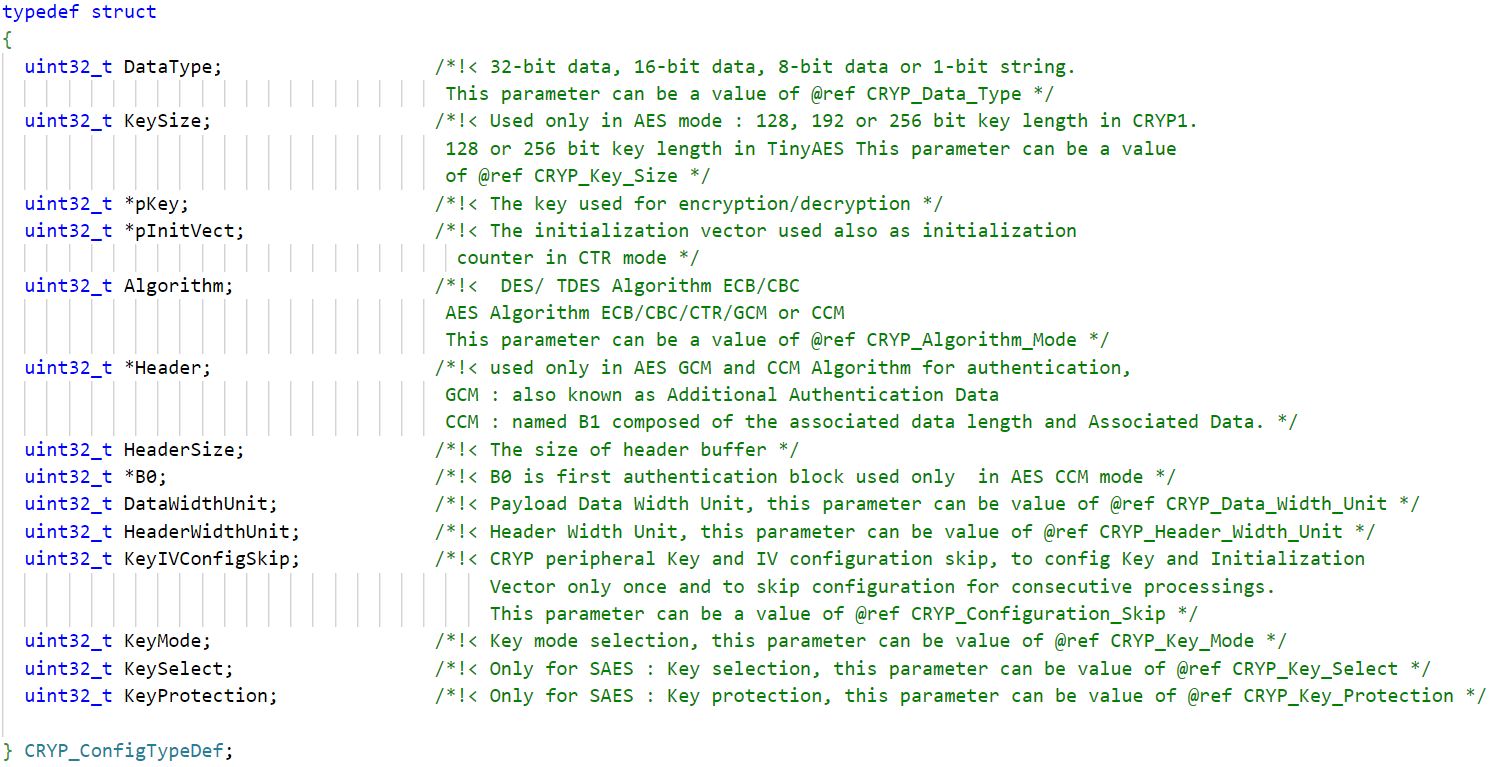
\includegraphics[width=18cm]{img/aes struct.png}
        \caption{AES HAL Structure}
    \label{fig:aes struct}
    \end{figure}

    \begin{figure}[H]
    \centering
    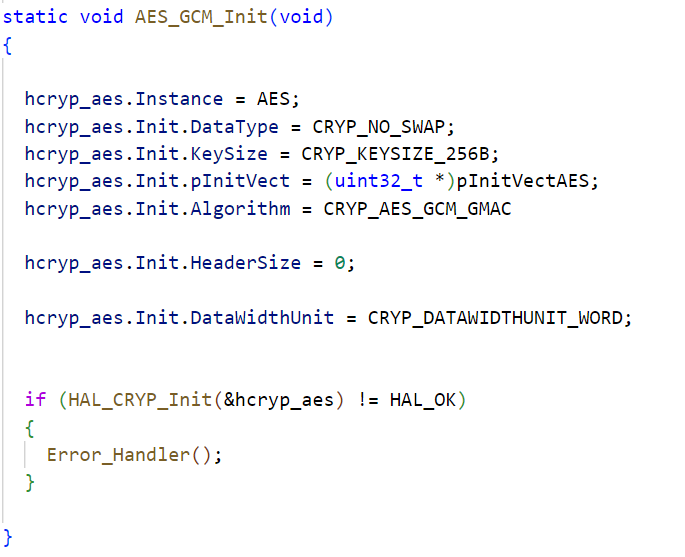
\includegraphics[width=10cm]{img/aes init.png}
        \caption{AES Structure Initialization}
    \label{fig:aes init}
    \end{figure}

    All that is left is to derive the AES key and initialization vector from the ECDH shared secret as shown in Figure \ref{fig:deriv}.
    
    \begin{figure}[H]
    \centering
    \includegraphics[width=12cm]{img/deriv.png}
        \caption{AES GCM Key and Initialization Vector Derivation}
    \label{fig:deriv}
    \end{figure}

    On the "Bob" side, we will encrypt and send the message "This is Bob" along with the tag that will help in verifying the integrity of the message. Figure \ref{fig:bob hello} demonstrates the plaintext, ciphertext and tag generated by the encryption process. Note that the "\%" symbol was added for extra padding since the AES peripheral expects a 128-bit input.

    \begin{figure}[H]
    \centering
    \includegraphics[width=12cm]{img/bob hello.png}
        \caption{AES GCM Key and Initialization Vector Derivation}
    \label{fig:bob hello}
    \end{figure}

    \subsection{Message Decryption and Tag Verification}
    The two devices exchange the encrypted messages and the generated tags. They must now decrypt the message while regenrating a tag. If the received tag is the same as the generated decryption tag, that means the message has been decrypted succesfully. Figure \ref{fig:tag} shows the decryption process on the "Bob" side which shows the correct decryption of the "Alice" message ("This is Alice").
    
    \begin{figure}[H]
    \centering
    \includegraphics[width=14cm]{img/end of demo.png}
        \caption{Message Decryption Output}
    \label{fig:tag}
    \end{figure}
The matching of the tags proves that the message was transmitted correctly and without any manipulation. It also ensures that the two sides have managed to derive the exact same symmetric key from the shared secret generation process, meaning that a secure line of communication has been succesfully established between the two devices.
\section*{Conclusion}
This chapter provided a comprehensive review of the implementation steps for the "CryptoEngine" demo, which demonstrates secure communication between two microcontrollers using cryptographic techniques. We explored the generation and exchange of cryptographic keys, including ECDSA and ECDH keys, and the processes of signature generation, verification, and secure message exchange using AES GCM. We also included relevant code snippets and expected outputs for each step of the demonstration to provide a complete overview.
        \clearpage
        
       %\chapter*{Conclusion}
\addcontentsline{toc}{chapter}{Conclusion}
\markboth{Conclusion}{}

This project aimed to develop a demonstration for the "CryptoEngine", a recent addition to the STM32 security portfolio. Conducted under the guidance of the ST Support Solutions team, our primary goal was to create a comprehensive yet accessible guide for customers interested in adopting this advanced technology. We set out to offer a practical example that balances showcasing the new features of the "CryptoEngine" while remaining simple enough to serve as an introduction to cryptography on STM32 microcontrollers.

Our objectives centered around providing a framework for constructing a secure encrypted communication system using the "CryptoEngine" 
 while illustrating the enhanced capabilities of this technology compared to existing solutions and promoting a deeper understanding of cryptographic principles through practical application. By the end of the project, we achieved these objectives by successfully implementing various cryptographic techniques, including symmetric encryption, key exchange mechanisms, and digital signatures, directly on STM32 hardware.

From a personal perspective, this project has provided an invaluable introduction to the fields of cryptography and embedded security. The experience has strengthened my understanding of cryptographic techniques and allowed me to apply this knowledge in practical settings, gaining insight into how these techniques protect data in embedded systems. I also gained a clearer perspective on the intricacies of secure communications, which is crucial in today's increasingly interconnected and digital world.

Furthermore, this project has served as a unique opportunity to understand the workflow within a company specializing in microcontrollers, revealing the complexities and nuances of working in such an environment. It has offered a closer look at the challenges and rewards of developing secure embedded systems, and has underscored the importance of collaboration, precise documentation, and iterative testing in delivering robust, reliable solutions.

Overall, this project has been both a professional and personal milestone, serving as a solid foundation for further exploration and specialization in cryptography and embedded security.
       %\clearpage
        
        % @author: Stoufa
		% the command `\nocite{*}` is mandatory to avoid the “no \citation commands” error
        % https://tex.stackexchange.com/questions/18045/problem-with-compiling-bibtex-no-citation-commands-error
        \nocite{*}
        \printbibliography[heading=bibintoc]
        
        \chapter*{Annexes}
\addcontentsline{toc}{chapter}{Annexes}
\markboth{Annexes}{}
\stepcounter{chapter}
\addtocontents{lot}{\vspace{3.8mm}}
\addtocontents{lof}{\vspace{3.8mm}}

%Mettez vos annexes ici...

%===================== ANNEXE 1 =====================%
\section*{Annexe 1.~Exemple d'annexe}
\addcontentsline{toc}{section}{Annexe 1.~Exemple d'annexe}

Les chapitres doivent présenter l’essentiel du travail. Certaines informations-trop  détaillées  ou constituant un complément d’information pour toute personne qui désire mieux comprendre ou refaire une expérience décrite dans le document- peuvent être mises au niveau des annexes. Les annexes, {\bf placées après la bibliographie}, doivent donc être numérotées avec des titres (Annexe1, Annexe2, etc.).

\addcontentsline{lot}{table}{Annexe 1.1~~~Exemple tableau dans l'annexe}

Le tableau annexe 1.1 présente un exemple d'un tableau dans l'annexe.

{\raggedright \textbf{Tableau annexe 1.1:}~Exemple tableau dans l'annexe}
\begin{longtable}[c]{
    | p{.20\textwidth}
    | p{.50\textwidth} |
}
    \hline
        0 & 0 \\ \hline 
        1 & 1 \\ \hline 
        2 & 2 \\ \hline
        3 & 3 \\ \hline
        4 & 4 \\
    \hline

\end{longtable}

\newpage
%===================== ANNEXE 2 =====================%
\section*{Annexe 2.~Entreprise}
\addcontentsline{toc}{section}{Annexe 2.~Entreprise}

\addcontentsline{lof}{figure}{Annexe 2.1~~~Logo d'entreprise}

La figure annexe 2.1 présente le logo entreprise.
\begin{figure}[htpb]
    \centering
    \frame{\includegraphics[width=0.45\columnwidth]{Logo_Entreprise}}
    {\\\textbf{Figure annexe 2.1:} Logo d'entreprise}
\end{figure}
        \clearpage

    \backmatter
        %===== File containing the back cover of the document =====%
%                                                          %
% Copyright (C) ISI - All Rights Reserved                  %
% Proprietary                                              %
% Written by Med Hossam <med.hossam@gmail.com>, April 2016 %
%                                                          %
% @author: HEDHILI Med Houssemeddine                       %
% @linkedin: http://tn.linkedin.com/in/medhossam           %
%==========================================================%

%== It's advised to not modify the content of this file ===%
% To set your information, go to global_config.tex file    %
%==========================================================%

\thispagestyle{backcover}
\newgeometry{bottom=25mm,left=15mm,top=20mm,right=15mm}

\begin{changemargin}{3mm}{0cm}
\vspace*{\fill}
    \begin{minipage}[c]{0.96\columnwidth}
        
       %\vspace{4cm}
        
        
        {\ifthenelse{\boolean{wantToTypeCompanyAddress}}
        {% IF TRUE
            \vskip5mm
        }
        
        \selectlanguage{english}
        {\LARGE\textbf{Abstract}}
        \vskip1mm
            \begingroup
                \large
                \@englishAbstract
            \endgroup
        \vskip1mm
        {\textbf{Keywords : }
            \begingroup
                \@englishAbstractKeywords
            \endgroup
        }
        {\vskip8mm}}
        
        \selectlanguage{french}
        
        {\LARGE\textbf{Résumé}}
        \vskip1mm
            \begingroup
                \large
                \@frenchAbstract
            \endgroup
        \vskip1mm
        {\textbf{Mots clés : }
            \begingroup
                \@frenchAbstractKeywords
            \endgroup
        }
    \end{minipage}
    \vspace*{\fill}
\end{changemargin}
    
\end{document}





